\documentclass[a4paper,12pt,twoside,openright]{book}

\raggedbottom

\usepackage[T1]{fontenc}
\usepackage[utf8]{inputenc}
\usepackage[english]{babel}
\usepackage{lmodern}
\usepackage{microtype}
\usepackage{geometry}
\usepackage{setspace}
\usepackage{graphicx}
\usepackage{float}
\usepackage{array}
\usepackage{booktabs}
\usepackage{amsmath,amssymb}
\usepackage{siunitx}
\usepackage{tikz}
\usepackage{hyperref}
\usepackage{cleveref}
\usepackage{csquotes}
\usepackage[backend=biber,style=numeric,sorting=none]{biblatex}
\usetikzlibrary{arrows.meta,positioning,calc}

\geometry{
  a4paper,
  inner=3.5cm,
  outer=2.5cm,
  top=3cm,
  bottom=3cm
}

\onehalfspacing
\graphicspath{{figures/}}
\addbibresource{references.bib}

\hypersetup{
  colorlinks=true,
  linkcolor=black,
  citecolor=black,
  urlcolor=blue,
  pdftitle={Machine Learning for Satellite Link Fade Nowcasting},
  pdfauthor={Giuseppe Gabriele Russo}
}

\newcommand{\planningnote}[1]{%
  \par\noindent\textit{#1}\par\medskip
}

\begin{document}

\frontmatter
\begin{titlepage}
  \centering

  \vspace*{0.4cm}
  
\includegraphics[width=2.6cm]{cherubino_pant541.png}\par
  \vspace{0.45cm}
  {\Large\textsc{University of Pisa}\par}
  \vspace{0.35cm}
  {\large Master's Degree in Computer Science\\Curriculum: Artificial Intelligence\par}

  \vfill

  {\large Master's Thesis\par}
  \vspace{0.75cm}
  \rule{0.78\textwidth}{0.4pt}\par
  \vspace{0.6cm}
  {\LARGE\bfseries Machine Learning for Satellite Link Fade Nowcasting\par}
  \vspace{0.6cm}
  \rule{0.78\textwidth}{0.4pt}\par

  \vfill

  \noindent
  \begin{minipage}[t]{0.45\textwidth}
    \raggedright
    \textbf{Supervisor}\\
    Davide Bacciu\\[0.35cm]
    \textbf{Co-supervisor}\\
    Giovanni Scognamiglio
  \end{minipage}
  \hfill
  \begin{minipage}[t]{0.45\textwidth}
    \raggedleft
    \textbf{Candidate}\\
    Giuseppe Gabriele Russo\\
    Student ID 583744
  \end{minipage}

  \vfill

  {\large Academic Year 2025/2026\par}
\end{titlepage}

\chapter*{Abstract}
\addcontentsline{toc}{chapter}{Abstract}

Satellite communication links may experience fade events that degrade the
received signal and require the activation of a backup communication resource.
In this setting, the relevant objective is not only to predict the future
signal accurately, but to support a timely switch decision using only
information available at the current time. This thesis studies satellite link
fade nowcasting as a decision-oriented time-series problem.

The work develops a reproducible signal-only machine-learning framework for
satellite fade data acquired at the Fucino ground station. The raw files are
standardized, cleaned, segmented, and converted into task-specific supervised
datasets. An external holdout source is kept separate from the development
data to evaluate generalization to an unseen acquisition file. A common
Perfect Switch reference and shared post-processing procedure are used to
compare models through operational switch metrics rather than only through
native prediction losses.

Four task formulations are investigated: autoregressive forecasting of the
future signal trajectory, current-level persistence regression, long-fade
detection, and survival persistence modeling. The evaluated model families
include GRU forecasting models, PatchTST, Chronos zero-shot forecasting,
XGBoost baselines, learnable shapelet models, temporal convolutional networks,
XGBoost-AFT, and a discrete-time survival TCN.

The results show that native predictive accuracy alone is not sufficient to
assess operational usefulness. Forecast errors, duration errors,
classification scores, and survival metrics are useful diagnostics, but final
switch quality depends on the formulation, conversion rule, and
post-processing. XGBoost-based current-level persistence provides a precise
and conservative switch policy, while XGBoost-AFT survival persistence offers
a stronger recall-oriented residual-duration formulation. PatchTST is the
strongest autoregressive switch model, whereas long-fade detection is more
appropriate as a high-recall warning mechanism than as a final controller.
Overall, satellite fade nowcasting should be evaluated as a complete decision
pipeline in which modeling choices and operational switch metrics are
inseparable.

%\chapter*{Acknowledgements}
\addcontentsline{toc}{chapter}{Acknowledgements}

I would like to thank my supervisor, Davide Bacciu, for his guidance,
feedback, and support throughout this thesis. I am also grateful to my
co-supervisor, Giovanni Scognamiglio, for the technical discussions and for
helping me refine the experimental direction of the work.

I would like to thank the people who provided access to the data and the
context needed to understand the operational problem addressed in this thesis.
Their contribution made it possible to study satellite fade nowcasting on real
signal measurements rather than on a purely synthetic setting.

Finally, I thank my family and the people close to me for their patience and
support during this work. Their encouragement was essential throughout the
development of the project and the writing of this thesis.


\tableofcontents
\listoffigures
\listoftables

\mainmatter
\chapter{Introduction}
\label{chap:introduction}

Satellite communication links are affected by propagation impairments that can
temporarily reduce the received signal quality. This problem is especially
relevant at high frequencies, where atmospheric phenomena such as rain can
produce strong fades on Earth-space paths \cite{panagopoulos2004satellite,
iturP618}. In operational systems, a fade is not only a physical phenomenon to
be described after it occurs. It is also a decision problem: when the primary
link degrades, an operator or automated controller may need to activate a
backup communication resource. Activating this resource too late may lead to
service degradation, while activating it too often or for too long may waste
capacity and increase operational cost.

The central question of this thesis is therefore not simply whether the future
satellite signal can be predicted. The more relevant question is whether
information available at the current time can support a timely and reliable
switch decision. This distinction changes how the problem should be modelled
and evaluated. A model with a low forecast error is not necessarily a good
switch controller if its errors occur around the operational threshold. A
model that estimates a duration or a probability may be more useful than a
trajectory forecaster if that quantity is more directly connected to the
decision. For this reason, the thesis treats satellite fade nowcasting as a
decision-oriented time-series problem.

\section{Operational Motivation}
\label{sec:introduction-operational-motivation}

Fade mitigation techniques are commonly used to preserve link availability
under adverse propagation conditions. Depending on the system, mitigation may
involve power control, adaptive coding and modulation, site diversity, or the
activation of an alternative link. The specific mitigation mechanism is outside
the scope of this thesis. The focus here is the upstream decision that such a
mechanism requires: given the signal observed up to the current timestamp,
should the system switch to a backup resource?

This decision has an intrinsically temporal structure. A very short threshold
crossing may not justify a switch, because the system could recover before the
backup activation becomes useful. Conversely, a fade that persists for several
minutes may justify switching even if the instantaneous signal is not at its
worst point yet. The operational objective is therefore tied to persistence,
residual duration, and event evolution, not only to the instantaneous signal
level. This is consistent with the broader propagation literature, where fade
dynamics and time-series behavior are treated as relevant design quantities
for Earth-space communication systems \cite{iturP1623,iturP1853}.

This thesis was carried out at M.B.I. S.r.l. \cite{mbiGroup} within the broader
context of the NEFOCAST project, for which M.B.I. is the lead company. NEFOCAST
investigates an integrated technological platform for estimating rainfall
fields from satellite-signal attenuation measurements
\cite{nefocastProject}. This industrial and research setting provides the
application context for the
decision-oriented nowcasting problem addressed in this work.

The data used in this work consist of signal time series acquired at the
Fucino ground station from multiple files and time periods. The available files
are heterogeneous: some are uplink or downlink beacon measurements, some are
associated with different satellites, and only a subset contains auxiliary
columns. To make the experimental comparison reproducible and fair, the thesis
adopts a strict signal-only policy. Every dataset is standardized to a common
time and signal representation, and all models use only the historical signal
as input. This avoids comparing models that have access to different physical
variables and keeps the focus on what can be learned from the signal evolution
itself.

\section{Satellite Link Fade Nowcasting}
\label{sec:introduction-nowcasting-problem}

Nowcasting refers to short-term prediction at or near the present time. In this
work, the prediction time is a timestamp \(t\) in a satellite signal time
series. The information available to a model is the recent past and present
signal history, while the target concerns the future behavior of the same
signal or of the ongoing fade event. No future observation can be used as an
input. This no-leakage constraint is essential because the final goal is an
operational decision that could be made online.

The thesis investigates four task formulations that all serve the same final
switching objective but estimate different intermediate quantities:

\begin{itemize}
  \item autoregressive forecasting, where the model predicts a future signal
  trajectory;
  \item current-level persistence, where the model estimates how long the
  signal will remain close to its current level;
  \item long-fade detection, where the model estimates whether the current
  grouped fade event will last longer than an operational duration threshold;
  \item survival persistence, where the model estimates a residual-duration
  survival function for the ongoing fade event.
\end{itemize}

These formulations are not interchangeable. They answer different operational
questions and produce different native outputs: trajectories, scalar
durations, class probabilities, or survival curves. To compare them, the
outputs must be converted into binary switch sequences and evaluated against a
common reference. This thesis therefore builds a shared Perfect Switch
reference, applies common switch post-processing, and reports operational
metrics in addition to native model metrics.

\section{Research Questions}
\label{sec:introduction-research-questions}

The work is guided by four research questions.

\begin{enumerate}
  \item \textbf{Can task-specific machine-learning models improve operational
  switch decisions for satellite link fades?} The objective is to evaluate
  whether learned models produce switch sequences that are closer to the
  reference decision than simple threshold reasoning.

  \item \textbf{Which predictive formulation is most useful for the switching
  objective?} The thesis compares trajectory forecasting, duration regression,
  event-level classification, and survival modeling because the best
  formulation is not obvious a priori.

  \item \textbf{Do native predictive metrics explain operational usefulness?}
  Forecast RMSE, duration MAE, classification AUPRC, and survival metrics are
  informative, but the final decision depends on thresholding,
  post-processing, and event timing. The thesis therefore studies how native
  metrics relate to switch metrics.

  \item \textbf{How important are common reference construction and
  post-processing?} Since different tasks produce outputs on different
  timestamp domains and with different semantics, the comparison must separate
  modeling differences from evaluation artifacts.
\end{enumerate}

These questions deliberately place the switch decision at the centre of the
study. The intermediate predictions remain important, but they are evaluated
as components of a decision pipeline rather than as isolated forecasting
outputs.

\section{Contributions}
\label{sec:introduction-contributions}

The main methodological and empirical contributions of the thesis are the
following.

\begin{enumerate}
  \item It formulates satellite fade nowcasting as a decision-oriented problem
  through four complementary predictive tasks: autoregressive forecasting,
  current-level persistence, long-fade detection, and survival persistence.
  Each task estimates a different intermediate quantity but is connected
  explicitly to the same operational switch objective.

  \item It establishes a shared switch-evaluation framework with a common
  Perfect Switch reference, shared post-processing, task-native comparisons,
  and a cross-task reference-grid comparison. This framework makes models with
  different native outputs operationally comparable.

  \item It evaluates a range of model families under these formulations,
  including GRU models, PatchTST, Chronos zero-shot forecasting, XGBoost
  baselines, learnable shapelet models, temporal convolutional networks,
  XGBoost-AFT, and a discrete-time survival TCN.

  \item It provides an empirical analysis of the relationship between native
  prediction quality and operational switch quality. The results show that the
  best native predictor is not always the best switch controller and that task
  formulation strongly affects the precision-recall trade-off.

  \item To support reproducibility, it develops a signal-only preprocessing
  pipeline for heterogeneous satellite fade and beacon files. The pipeline
  validates and standardizes raw data, handles gaps conservatively, constructs
  task-specific datasets, and preserves the metadata required for event-level
  evaluation.
\end{enumerate}

The source-code repository for the experimental framework is hosted on GitHub:
\url{https://github.com/Giusgarus/Nowcasting-project}.
It contains the task implementations, experiment configurations, and evaluation
scripts used in this work.

\section{Thesis Structure}
\label{sec:introduction-structure}

\Cref{chap:background} introduces the technical background needed for the
work. It covers time-series data, machine-learning models used in the thesis,
survival analysis, nowcasting and validation principles, and the satellite
communication context.

\Cref{chap:data-reference-framework} describes the data preparation and
reference-decision framework. It explains the available signal files, the
signal-only policy, parsing and validation, sampling gaps, conservative
imputation, event construction, the external holdout split, the Perfect Switch
reference, and the shared switch post-processing rules.

\Cref{chap:task-formulations} presents the four modeling formulations. For
each formulation, it defines the input representation, target construction,
model families, native output, and switch-conversion rule.

\Cref{chap:experimental-setup} describes the experimental protocol, including
dataset construction, train-validation-test usage, hyperparameter search,
native metrics, switch metrics, intra-task comparisons, cross-task
comparisons, and reproducibility settings.

\Cref{chap:results} reports and discusses the empirical results. It first
analyses the native predictive performance within each task and then focuses
on the switch metrics and event-level behavior that determine operational
usefulness.

\Cref{chap:conclusions} summarizes the main findings, answers the research
questions, discusses limitations, and outlines future work.

\chapter{Background}
\label{chap:background}

Before the individual nowcasting tasks can be defined, two questions have to be
made explicit: what kind of object a time series is, and what assumptions are
introduced when it is transformed into supervised learning data. The background
therefore starts from time-indexed observations, with emphasis on ordering,
sampling, windowing, and the risk of temporal leakage. It then reviews the
machine-learning model families used later in the thesis at the level of their
modeling mechanisms rather than as task-specific experimental choices. On this
basis, a separate section defines the nowcasting problem and the validation
principles needed to assess temporal generalization. The final part returns to
the satellite-link setting, where the technical modeling
problem becomes an operational decision about whether a backup link should be
activated. Detailed model instantiations are left to
\cref{chap:task-formulations}, while training, selection, and evaluation
procedures are left to the experimental setup chapter.

\section{Time Series as Data}
\label{sec:background-time-series}

\subsection{Time Index and Information Order}

A time series is not merely a table with a timestamp column. It is a realization
of a temporal process observed at ordered time instants
\cite{brockwell2016introduction,shumway2017time}. In the setting considered in
this thesis, each observation consists of a timestamp \(t_i\) and a scalar signal
value \(S_i\):
\[
  \{(t_i,S_i)\}_{i=1}^{N},
  \qquad
  t_1 < t_2 < \cdots < t_N .
\]
Equivalently, the measured signal can be interpreted as samples from an
underlying process \(S(t)\), observed only at the finite set of times
\(\{t_i\}_{i=1}^{N}\). The temporal index is therefore part of the data
definition. Two sequences containing the same numerical values but arranged in a
different order can describe different physical evolutions.

Let \(\mathcal{F}_i\) denote the information available at time \(t_i\).
Formally, it is the sigma-algebra generated by \(S_1,\ldots,S_i\): the smallest
sigma-algebra with respect to which these random variables are measurable.
A causal nowcasting model must base its decision at \(t_i\) only
on \(\mathcal{F}_i\). This notation is useful because it separates the offline
construction of labels from the online information set. Future observations may
be used after the fact to define a supervised target, namely the outcome the
model is trained to predict, but they are not part of the information available
when the operational decision is made.

This makes time-series data different from ordinary exchangeable tabular data.
In a tabular classification problem, the rows are often treated as independent
or at least exchangeable after conditioning on their features. In a time series,
row \(i+1\) is not an arbitrary new case: it is the continuation of the same
temporal evolution observed at row \(i\). Models, preprocessing steps, and
validation protocols must respect this direction of time.

\subsection{Temporal Dependence and Non-Stationarity}

Consecutive samples in a time series are statistically dependent. In a satellite-link
signal, the value at \(t_i\) is informative about nearby future values because
atmospheric and equipment states evolve continuously rather than being redrawn
independently at each timestamp. This temporal dependence is the basic reason
why forecasting methods use past observations as input features
\cite{hyndman2021forecasting}.

For a regularly sampled univariate series, second-order temporal dependence is
often summarized through the autocovariance and autocorrelation functions
\cite{shumway2017time}. If the process is weakly stationary, with constant mean
\(\mu\) and variance, the lag-\(k\) autocovariance is
\[
  \gamma(k)
  =
  \operatorname{Cov}(S_i,S_{i-k})
  =
  \mathbb{E}\left[(S_i-\mu)(S_{i-k}-\mu)\right],
\]
and the autocorrelation is
\[
  \rho(k) = \frac{\gamma(k)}{\gamma(0)} .
\]
Positive autocorrelation at small lags means that recent values carry
predictive information about the next samples. For fade nowcasting, this local
dependence is central: an above-threshold sample is operationally more important
when it occurs inside a persistent fade trajectory than when it is an isolated
fluctuation.

Stationarity is a useful reference concept, but real measurement series often
violate it. A strictly stationary process has joint distributions that are
invariant under time shifts, while weak stationarity requires constant first and
second moments and autocovariances that depend only on lag. Satellite-link data
can depart from these assumptions because weather regimes, seasonal effects,
receiver conditions, maintenance interventions, and acquisition quality can
change over long periods. A model trained on one part of the acquisition history
may therefore face a different distribution later in time.

Fade-related signals also combine dense ordinary behavior with sparse
operationally relevant events. Most timestamps may correspond to acceptable link
conditions, while the samples near or above an operational threshold determine
whether a backup link should be activated. This creates an imbalance between
global signal reconstruction and decision relevance. A small numerical error far
from the threshold may have little operational effect, whereas a similar error
near the threshold can change the switch decision.

\subsection{Sampling Cadence, Gaps, and Acquisition Segments}

Time-series models often operate on index steps, but the physical process
evolves in elapsed time. Let
\[
  \Delta_i = t_i - t_{i-1}
\]
be the interval between two consecutive observations. When \(\Delta_i\) is
approximately constant, a context of \(L\) samples corresponds to a stable
look-back duration of roughly \(L\Delta_i\). When the intervals are irregular or
large gaps appear, the same number of samples can correspond to very different
amounts of physical time.

This distinction matters for both inputs and targets. If a gap of several
minutes is treated as a normal one-step transition, the model receives a
distorted representation of the signal dynamics. The same issue affects label
construction: a later observation after a long acquisition gap is not evidence
that the signal persisted continuously through the missing interval. Missing
observations are therefore not only a data-cleaning inconvenience; they change
what can be inferred about duration, recovery, and event continuity.

Within the scope of this thesis we distinguish sample order from continuous
acquisition. A continuous acquisition segment is a portion of the series where
the sampling cadence is regular enough to support windowed modeling and target
construction. Context windows must remain inside such segments. Conservative
short-gap imputation can be useful when the missing interval is small and
explicitly bounded, but it should not bridge long gaps or merge distinct
acquisition segments. This principle is methodological rather than
model-specific: every downstream task depends on the same interpretation of
time.

Sampling cadence also determines the temporal meaning of a prediction horizon.
A horizon of ten samples is not intrinsically a ten-step operational forecast;
under a 30-second cadence, it corresponds to approximately five minutes. The
same horizon would have a different meaning under a different cadence. For this
reason, time-series experiments must report both sample-based and time-based
interpretations when the operational decision depends on elapsed duration.

\subsection{Windowed Supervised Learning}

In supervised learning, a dataset consists of input--target pairs \((X_i,Y_i)\).
The input \(X_i\) contains the information supplied to the model, while the
target \(Y_i\) provides the observed outcome, or the available information about
that outcome, used to supervise learning. The task definition determines how
the target is constructed from the recorded data.

A time series is converted into such examples by applying a sliding-window
transformation to the ordered observations and associating each window with its
target. For a decision made at index \(i\), a context of length \(L\) is
\[
  X_i = [S_{i-L+1}, \ldots, S_i].
\]
The last value \(S_i\) is the newest signal value available when the decision is
made. Given this input, a model produces a prediction through the mapping
\[
  z_i = f_\vartheta(X_i),
\]
where \(z_i\) is the task-specific output and \(\vartheta\) denotes learned or
pretrained parameters. The output may be a future trajectory, a scalar duration,
a class probability, or a survival curve.

The prediction \(z_i\) and the target \(Y_i\) have distinct roles: the former is
computed by the model, while the latter supplies the supervision. During
training, a task-specific loss function measures how well the model output
agrees with the target. Their representations need not be identical. A binary
classifier can output a probability while its target is a class label; a
survival model can output a curve while its target records a follow-up duration
and whether the event was observed or censored.

For example, in multi-step forecasting with horizon \(h\), the target is the
observed future trajectory,
\[
  Y_i = [S_{i+1},S_{i+2},\ldots,S_{i+h}] .
\]
The corresponding model output \(z_i\) is a predicted trajectory, denoted by
\(\widehat{Y}_i\), which is compared with \(Y_i\) during training and evaluation.
If a regularly sampled segment contains \(N_s\) observations, the number of
valid fully observed forecasting windows with unit stride is
\[
  N_{\mathrm{win}} = N_s - L - h + 1 ,
\]
provided \(N_s \ge L+h\). This simple expression hides an important statistical
fact: adjacent windows are strongly overlapping. \(X_i\) and \(X_{i+1}\) share
\(L-1\) observations, so the resulting supervised rows are not independent even
if they are stored in a matrix.

The target may depend on future observations during offline dataset generation,
but the input must not. This is the central no-leakage constraint:
\[
  X_i \text{ and all input features at } t_i
  \text{ may depend only on } \{S_j : j \le i\}.
\]
Future observations can define supervision for offline learning and evaluation,
but they cannot enter the input features used for a decision at \(t_i\).
Fitted preprocessing parameters and model selection must also respect the
separation of training, validation, and test data discussed in
\cref{sec:background-validation}. The same input-time restriction applies to derived
features: a rolling mean, slope, threshold occupancy, or event-state feature is
valid only if it can be computed from the past and present observations
available at \(t_i\).

For multi-step forecasting, several strategies are possible
\cite{taieb2012review}. A recursive strategy trains a one-step-ahead predictor
and applies it repeatedly, feeding previous predictions back as inputs. A direct
strategy trains one predictor per forecast horizon. A multiple-output strategy
predicts the whole future vector in one pass. These strategies make different
assumptions about how errors propagate and about whether future horizons should
be modelled independently or jointly. The choice is therefore not just an
implementation detail: it determines the relation between the learned model, the
prediction horizon, and the operational switch rule applied later.

\section{Machine Learning for Time Series}
\label{sec:background-ml-time-series}

This section presents the theoretical foundations of the machine-learning model
families used in the experiments of this thesis. Its scope follows the
implemented approaches: gradient-boosted decision trees with XGBoost, GRU
recurrent networks, patch-based Transformers through PatchTST, the pretrained
Chronos forecasting model, learnable shapelet models, and temporal convolutional
networks. It also introduces the survival-analysis concepts underlying the
XGBoost-AFT and discrete-time TCN survival models.

For each family, the following subsections explain its mathematical formulation,
how it represents temporal information, and the assumptions that shape its
predictions, with reference to the relevant literature. These foundations
provide the terminology and notation for \cref{chap:task-formulations}, where
the models are assigned to the predictive tasks and their inputs, outputs, and
switch-conversion rules are specified. Training procedures, hyperparameter
selection, and evaluation protocols are described in
\cref{chap:experimental-setup}.

\subsection{Gradient-Boosted Decision Trees}
\label{sec:background-xgboost}

Gradient boosting builds an additive model by fitting weak learners
sequentially. The general idea was formalized by Friedman as gradient descent in
function space \cite{friedman2001greedy}. XGBoost is a regularized and scalable
implementation of boosted decision trees \cite{chen2016xgboost}. A tree ensemble
can be written as
\[
  F(\phi_i) = \sum_{m=1}^{M} f_m(\phi_i),
\]
where \(\phi_i\) is a tabular feature vector and \(f_m\) is an individual
decision tree. Each tree partitions the feature space into leaves and assigns a
constant score to each leaf. If \(q_m(\phi_i)\) denotes the leaf reached by
sample \(i\) in tree \(m\), then \(f_m(\phi_i)=w_{q_m(\phi_i)}\), where
\(w_j\) is the learned score of leaf \(j\).

\begin{figure}[htbp]
  \centering
  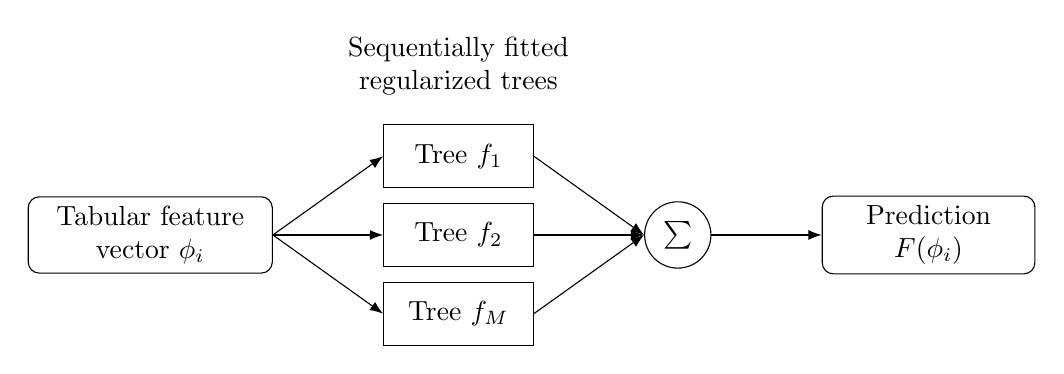
\begin{tikzpicture}[
      >=Latex,
      node distance=1.2cm,
      feature/.style={draw, rounded corners, align=center, minimum width=3.1cm, minimum height=0.9cm},
      tree/.style={draw, align=center, minimum width=1.9cm, minimum height=0.8cm},
      op/.style={draw, circle, align=center, minimum size=0.75cm},
      output/.style={draw, rounded corners, align=center, minimum width=2.7cm, minimum height=0.9cm}
    ]
    \node[feature] (features) {Tabular feature\\vector \(\phi_i\)};
    \node[tree, right=1.4cm of features, yshift=1.0cm] (tree1) {Tree \(f_1\)};
    \node[tree, right=1.4cm of features] (tree2) {Tree \(f_2\)};
    \node[tree, right=1.4cm of features, yshift=-1.0cm] (treem) {Tree \(f_M\)};
    \node[op, right=1.4cm of tree2] (sum) {\(\sum\)};
    \node[output, right=1.4cm of sum] (prediction) {Prediction\\\(F(\phi_i)\)};

    \draw[->] (features.east) -- (tree1.west);
    \draw[->] (features.east) -- (tree2.west);
    \draw[->] (features.east) -- (treem.west);
    \draw[->] (tree1.east) -- (sum.west);
    \draw[->] (tree2.east) -- (sum.west);
    \draw[->] (treem.east) -- (sum.west);
    \draw[->] (sum.east) -- (prediction.west);
    \node[align=center, above=0.25cm of tree1] {Sequentially fitted\\regularized trees};
  \end{tikzpicture}
  \caption{Schematic representation of an XGBoost tree ensemble. A tabular feature vector is evaluated by multiple decision trees, and their leaf scores are added to form the final prediction.}
  \label{fig:xgboost-ensemble}
\end{figure}

Training minimizes a predictive loss plus a regularization term on tree
complexity:
\[
  \mathcal{L}
  =
  \sum_i \ell(y_i, F(\phi_i))
  +
  \sum_{m=1}^{M}\Omega(f_m).
\]
In XGBoost, the regularization term penalizes both the number of leaves and
the magnitude of leaf scores:
\[
  \Omega(f_m) = \gamma T_m + \frac{1}{2}\lambda\sum_{j=1}^{T_m} w_j^2 ,
\]
where \(T_m\) is the number of leaves, \(\gamma\) penalizes additional leaves,
and \(\lambda\) shrinks leaf weights. This is important because boosted trees
can otherwise fit highly specific partitions of the training data, especially
when many lag features are derived from overlapping time windows.

At boosting iteration \(m\), the new tree is fitted to improve the current
prediction \(\widehat{y}^{(m-1)}_i\). XGBoost uses a second-order Taylor
approximation of the loss around the current prediction:
\[
  \mathcal{L}^{(m)}
  \simeq
  \sum_i
  \left[
    g_i f_m(\phi_i)
    +
    \frac{1}{2}h_i f_m(\phi_i)^2
  \right]
  +
  \Omega(f_m),
\]
where
\[
  g_i =
  \partial_{\widehat{y}^{(m-1)}_i}
  \ell(y_i,\widehat{y}^{(m-1)}_i),
  \qquad
  h_i =
  \partial^2_{\widehat{y}^{(m-1)}_i}
  \ell(y_i,\widehat{y}^{(m-1)}_i).
\]
The first derivative indicates the direction in which the prediction should be
corrected, while the second derivative scales that correction by local
curvature. For a candidate split, XGBoost compares the score of the parent node
with the scores of the two child nodes. If \(G\) and \(H\) are the sums of
gradients and Hessians in a node, the split gain has the form
\[
  \operatorname{Gain}
  =
  \frac{1}{2}
  \left[
    \frac{G_L^2}{H_L+\lambda}
    +
    \frac{G_R^2}{H_R+\lambda}
    -
    \frac{G^2}{H+\lambda}
  \right]
  -
  \gamma .
\]
Splits are therefore selected only when they reduce the regularized objective,
not merely when they improve the training loss locally.

For time-series data, a boosted tree does not process temporal order directly.
The ordered context must first be converted into a feature vector, for example
by flattening lagged signal values and adding scalar summaries of the recent
window:
\[
  \phi_i =
  [S_{i-L+1},\ldots,S_i,\eta_1(X_i),\ldots,\eta_p(X_i)] ,
\]
where \(\eta_1,\ldots,\eta_p\) are optional summaries computed only from the
available context, such as recent slopes or window statistics. In this
representation, temporal order is encoded by feature position: the model can
distinguish \(S_i\) from \(S_{i-10}\), but it has no built-in notion that these
features are adjacent samples. This is both a limitation and a strength. It is a
limitation because the model does not share parameters across time and does not
learn a recurrent state. It is a strength because decision trees can create
piecewise rules involving specific lags, levels, and interactions, such as a
large current signal combined with a positive recent slope.

The same ensemble mechanism can be paired with different losses. Squared-error
or absolute-error variants support scalar regression; logistic objectives
support binary event classification; and the accelerated-failure-time objective
extends the framework to right-censored duration targets
\cite{xgboostAftDocs,barnwal2022xgboostAft}. In a nowcasting study, this makes
XGBoost useful in two roles. First, it is a strong tabular baseline that tests
how much information is already present in lagged signal values and simple
context summaries. Second, it provides a robust comparison point for neural
sequence models, because it avoids recurrent or attention-based optimization
while still modeling nonlinear threshold effects.

\subsection{Recurrent Sequence Models and GRUs}
\label{sec:background-gru}

Recurrent neural networks process a sequence one element at a time while
maintaining a hidden state.

\begin{figure}[htbp]
  \centering
  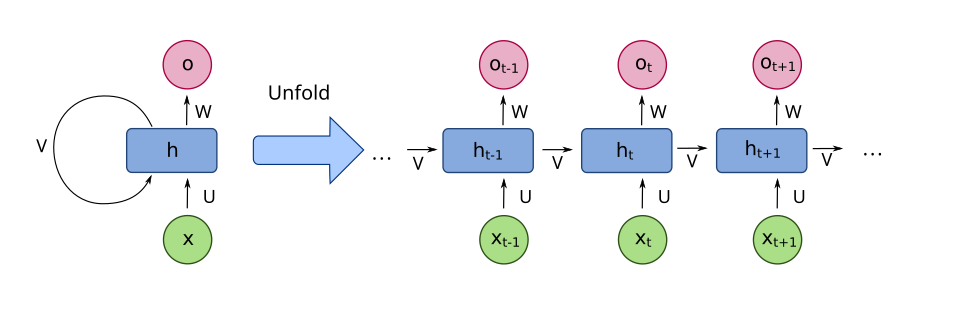
\includegraphics[width=0.82\textwidth]{figures/Recurrent_neural_network_unfold.png}
  \caption{Unfolded recurrent neural network processing a sequence through a hidden state. Source: \cite{fdeloche2017rnnunfold}.}
  \label{fig:rnn-unfolding}
\end{figure}

The basic recurrent idea is to represent time
implicitly through feedback in the hidden representation
\cite{elman1990finding}. At sequence position \(\ell\), a recurrent model can be
written as
\[
  h_\ell = \psi(x_\ell,h_{\ell-1}),
\]
where \(x_\ell\) is the current input and \(h_{\ell-1}\) summarizes the previous
part of the sequence. The hidden state is therefore a learned memory of the
past. A forward unidirectional recurrence processes the input window from its
oldest observation toward its most recent one.

A bidirectional recurrent network processes the supplied sequence in both
directions and combines the forward and backward representations
\cite{schuster1997bidirectional}. For a prediction issued at \(t_i\), both
directions can operate on the fully observed context
\(X_i=[S_{i-L+1},\ldots,S_i]\). The backward recurrence then uses observations
that are later than an internal window position, but all of them are already
available at \(t_i\). Bidirectional encoding of this past context is therefore
compatible with the no-leakage constraint. The relevant boundary is the time at
which the prediction is issued: using \(S_j\) with \(j>i\) to make that
prediction would violate the constraint. Likewise, a representation computed
using the entire window cannot be treated as available at an earlier position
inside that window if it depends on observations acquired after that position.

Plain recurrent networks can have difficulty learning long dependencies because
gradients may vanish or explode during backpropagation through time. Gated
architectures address this by controlling how information is stored and
updated. Long short-term memory networks introduced explicit memory cells and
gates \cite{hochreiter1997long}. Gated recurrent units simplify this idea while
retaining gates that regulate state updates.

\begin{figure}[htbp]
  \centering
  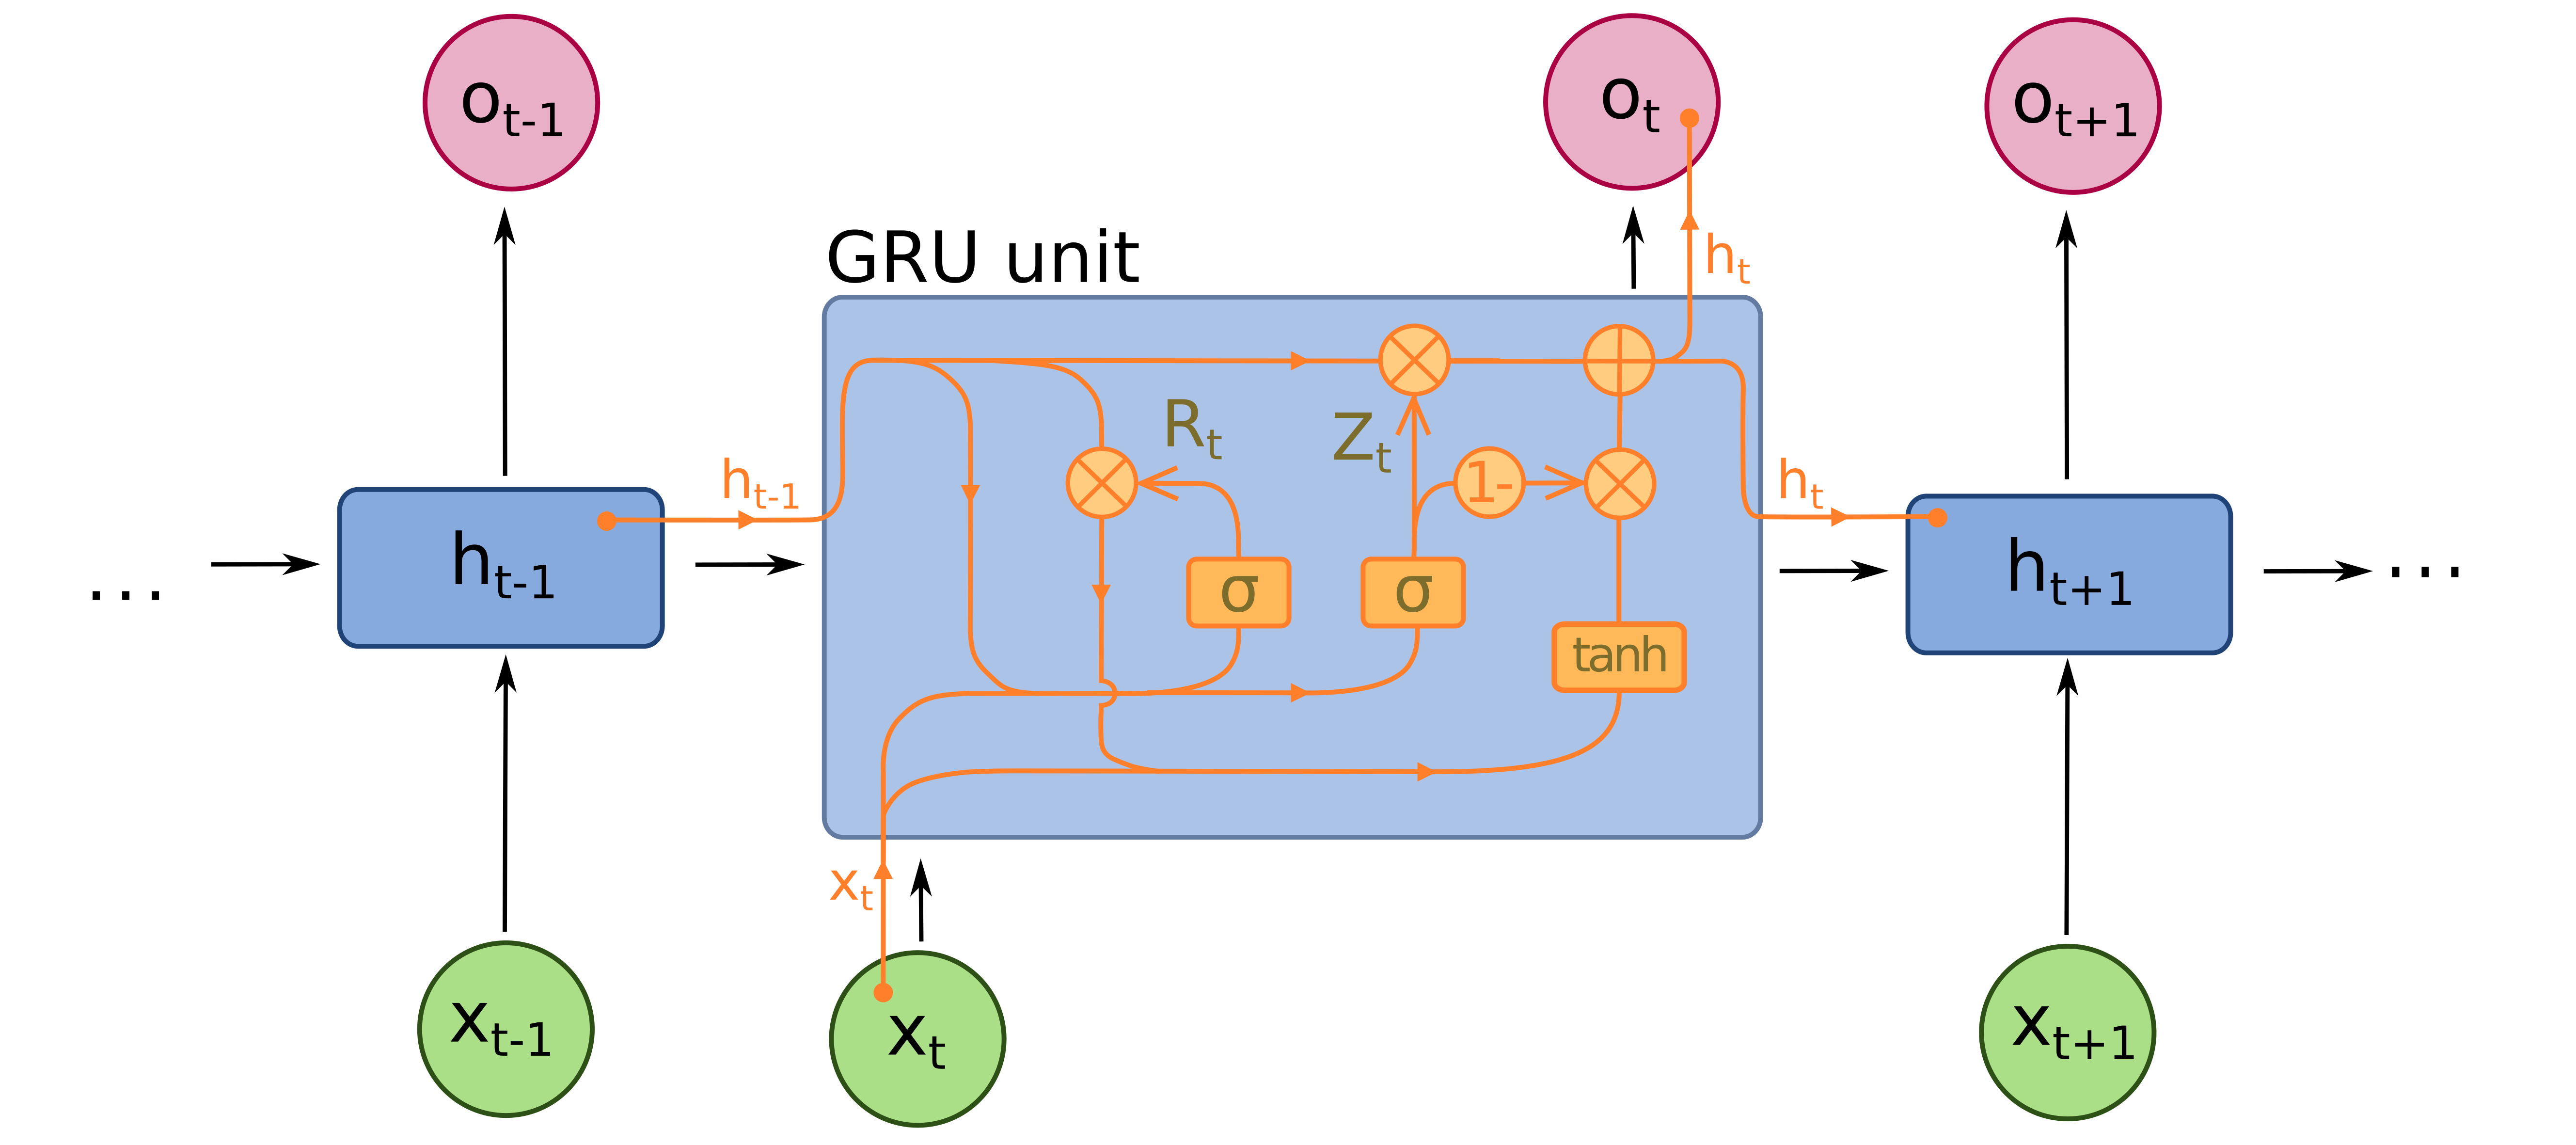
\includegraphics[width=0.82\textwidth]{figures/Gated_Recurrent_Unit.png}
  \caption{Structure of a gated recurrent unit. Source: \cite{fdeloche2017gru}.}
  \label{fig:gru-structure}
\end{figure}

GRUs were introduced in the context
of encoder-decoder sequence learning \cite{cho2014learning} and later evaluated
as general sequence modeling units \cite{chung2014empirical}.

Throughout this thesis, \(\sigma(\cdot)\) denotes the logistic sigmoid function,
\[
  \sigma(z)=\frac{1}{1+\exp(-z)},
\]
applied elementwise when its argument is a vector.

For a univariate input value \(x_t\), a GRU updates its hidden state
\(h_t\) using an update gate \(z_t\), a reset gate \(r_t\), and a
candidate state \(\widetilde{h}_t\):
\[
\begin{aligned}
  z_t &= \sigma(W_z x_t + U_z h_{t-1} + b_z), \\
  r_t &= \sigma(W_r x_t + U_r h_{t-1} + b_r), \\
  \widetilde{h}_t
  &= \tanh(W_h x_t + U_h(r_t \odot h_{t-1}) + b_h), \\
  h_t
  &= (1-z_t)\odot h_{t-1} + z_t\odot\widetilde{h}_t .
\end{aligned}
\]
The update gate controls how much of the candidate state replaces the previous
state, while the reset gate controls how much previous memory is used to form
the candidate. When \(z_t\) is small, the unit mostly preserves its previous
state; when \(z_t\) is large, it updates the memory toward the new candidate.
When \(r_t\) is small, the candidate is computed with little dependence on
older memory, allowing the unit to react to a local change. When \(r_t\) is
large, the candidate can use a longer effective history. In a fade-related
signal, these gates let the model represent whether the recent pattern resembles
a rising fade, a plateau, an oscillation, or a recovery without requiring
manually defined event states.

The hidden dimension controls the capacity of this memory. A very small hidden
state may compress different temporal patterns into similar representations,
whereas a large hidden state can overfit repeated windows from a limited number
of fade episodes. Stacking multiple GRU layers increases representational power:
lower layers can encode local signal transitions, while upper layers combine
those transitions into a coarser sequence representation. Dropout
\cite{srivastava2014dropout} and early stopping \cite{prechelt1998early}
are often used to limit overfitting, but they do not replace the need
for chronological validation because neighboring windows remain highly
correlated.

Two recurrent structures are common in multi-step forecasting. A
sequence-to-vector model encodes the whole context and maps the final hidden
state directly to an output vector:
\[
  \widehat{Y}_i = W_o a_L + b_o .
\]
This is a direct multiple-output forecast: all horizons are predicted from the
same encoded context. The advantage is that errors made for early horizons do
not have to be fed back into later horizons. The limitation is that the forecast
horizon is represented mainly through the output layer, so the model does not
explicitly simulate a future recurrent trajectory.

\begin{figure}[htbp]
  \centering
  \resizebox{0.96\textwidth}{!}{%
  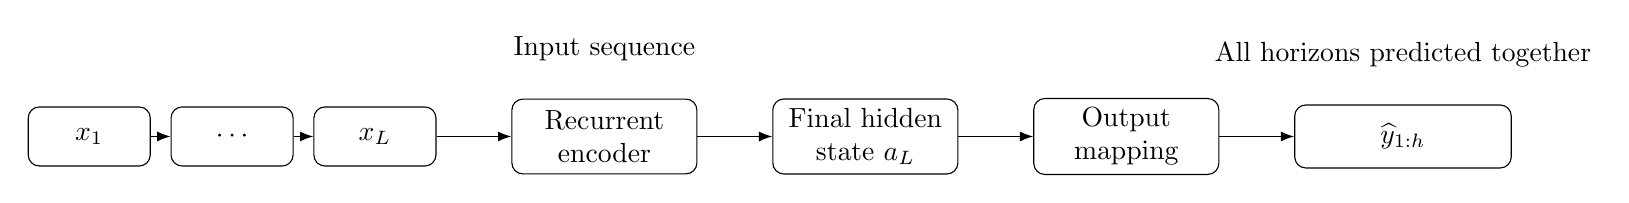
\begin{tikzpicture}[
      >=Latex,
      node distance=0.9cm and 1.0cm,
      sample/.style={draw, rounded corners, align=center, minimum width=1.55cm, minimum height=0.75cm},
      block/.style={draw, rounded corners, align=center, minimum width=2.35cm, minimum height=0.95cm},
      vector/.style={draw, rounded corners, align=center, minimum width=2.75cm, minimum height=0.8cm}
    ]
    \node[sample] (x1) {\(x_1\)};
    \node[sample, right=0.25cm of x1] (x2) {\(\cdots\)};
    \node[sample, right=0.25cm of x2] (x3) {\(x_L\)};
    \node[block, right=0.95cm of x3] (encoder) {Recurrent\\encoder};
    \node[block, right=0.95cm of encoder] (state) {Final hidden\\state \(a_L\)};
    \node[block, right=0.95cm of state] (head) {Output\\mapping};
    \node[vector, right=0.95cm of head] (forecast) {\(\widehat{y}_{1:h}\)};

    \draw[->] (x1.east) -- (x2.west);
    \draw[->] (x2.east) -- (x3.west);
    \draw[->] (x3.east) -- (encoder.west);
    \draw[->] (encoder.east) -- (state.west);
    \draw[->] (state.east) -- (head.west);
    \draw[->] (head.east) -- (forecast.west);

    \node[align=center, above=0.35cm of encoder] {Input sequence};
    \node[align=center, above=0.35cm of forecast] {All horizons predicted together};
  \end{tikzpicture}%
  }
  \caption{Generic sequence-to-vector recurrent forecaster. The input sequence is encoded once, and the final hidden state is mapped directly to a multi-step output vector.}
  \label{fig:sequence-to-vector-forecasting}
\end{figure}

An encoder-decoder model instead uses one recurrent network to encode the
observed context and another to decode future values step by step, following the
broader sequence-to-sequence framework \cite{sutskever2014sequence}. The decoder
state evolves over the prediction horizon,
\[
  d_k = \psi_{\mathrm{dec}}(\xi_k,d_{k-1}),
  \qquad
  \widehat{S}_{i+k}=W_d d_k+b_d ,
\]
where \(\xi_k\) is the decoder input at future step \(k\). During training,
\(\xi_k\) may be the previous true target value, a previous prediction, or a
mixture of the two, depending on the teacher-forcing strategy. During
evaluation, future true values are unavailable, so decoded predictions must be
generated using only the encoded context and previously generated outputs. This
gives the forecast horizon an explicit temporal structure, but it can also
propagate early prediction errors.

\begin{figure}[htbp]
\centering

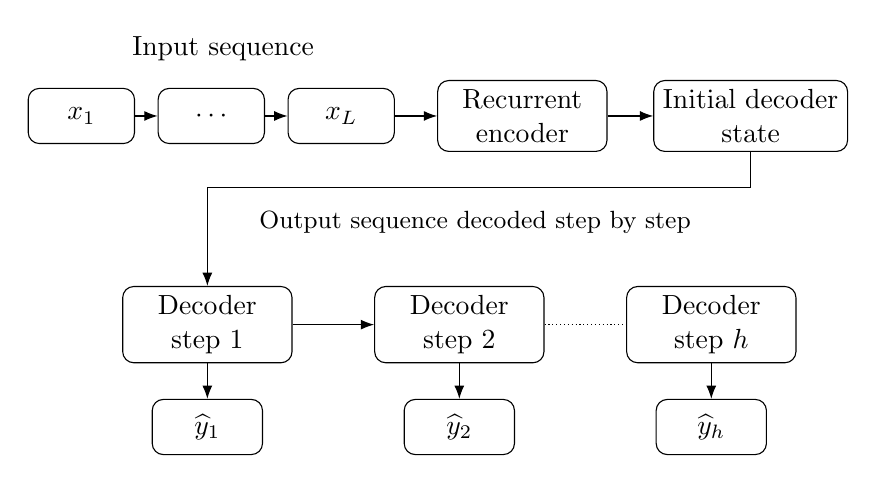
\begin{tikzpicture}[
    >=Latex,
    sample/.style={
        draw,
        rounded corners,
        align=center,
        minimum width=1.35cm,
        minimum height=0.7cm
    },
    block/.style={
        draw,
        rounded corners,
        align=center,
        minimum width=2.15cm,
        minimum height=0.9cm
    },
    forecastout/.style={
        draw,
        rounded corners,
        align=center,
        minimum width=1.4cm,
        minimum height=0.7cm
    }
]

% ------------------------------------------------
% Encoder
% ------------------------------------------------

\node[sample] (x1) at (-4.8, 1.3) {\(x_1\)};
\node[sample] (x2) at (-3.15, 1.3) {\(\cdots\)};
\node[sample] (x3) at (-1.5, 1.3) {\(x_L\)};

\node[block] (encoder) at (0.8, 1.3)
    {Recurrent\\encoder};

\node[block] (d0) at (3.7, 1.3)
    {Initial decoder\\state};

\node[align=center] at (-3.0, 2.15)
    {Input sequence};

% ------------------------------------------------
% Decoder
% ------------------------------------------------

\node[align=center, font=\small] at (0.2, -0.05)
    {Output sequence decoded step by step};

\node[block] (dec1) at (-3.2, -1.35)
    {Decoder\\step \(1\)};

\node[block] (dec2) at (0, -1.35)
    {Decoder\\step \(2\)};

\node[block] (dech) at (3.2, -1.35)
    {Decoder\\step \(h\)};

% ------------------------------------------------
% Outputs
% ------------------------------------------------

\node[forecastout] (y1) at (-3.2, -2.65)
    {\(\widehat{y}_1\)};

\node[forecastout] (y2) at (0, -2.65)
    {\(\widehat{y}_2\)};

\node[forecastout] (yh) at (3.2, -2.65)
    {\(\widehat{y}_h\)};

% ------------------------------------------------
% Connections
% ------------------------------------------------

\draw[->] (x1.east) -- (x2.west);
\draw[->] (x2.east) -- (x3.west);
\draw[->] (x3.east) -- (encoder.west);
\draw[->] (encoder.east) -- (d0.west);

% Initial decoder state -> first decoder step
\draw[->]
    (d0.south)
    -- ++(0,-0.45)
    -| (dec1.north);

% Autoregressive decoder evolution
\draw[->] (dec1.east) -- (dec2.west);
\draw[densely dotted] (dec2.east) -- (dech.west);

% Decoder outputs
\draw[->] (dec1.south) -- (y1.north);
\draw[->] (dec2.south) -- (y2.north);
\draw[->] (dech.south) -- (yh.north);

\end{tikzpicture}

\caption{Generic encoder-decoder recurrent forecaster.
The encoder summarizes the input sequence, while the decoder evolves over
the forecast horizon and emits one output at each step.}
\label{fig:encoder-decoder-forecasting}
\end{figure}

Compared with tree-based lag models, GRUs encode temporal order directly and
share recurrent parameters across positions in the window. This learned memory
of the available signal history makes them a natural baseline for testing
whether explicit sequence modeling improves over tabular lag features in
satellite fade nowcasting.

\subsection{Transformers and PatchTST}
\label{sec:background-patchtst}

Transformers represent sequences through attention rather than recurrence. The
core operation is scaled dot-product attention \cite{vaswani2017attention}:
\[
  \operatorname{Attention}(Q,K,V)
  =
  \operatorname{softmax}
  \left(
    \frac{QK^\top}{\sqrt{d_k}}
  \right)V .
\]
Queries, keys, and values are learned projections of input tokens. Attention
allows each token representation to combine information from other tokens in
the context.

This mechanism can now be compared with the GRU encoders introduced above.
A GRU updates its hidden state sequentially across context positions, whereas
a Transformer encoder can compute representations for all observed context
tokens in parallel within each layer \cite{vaswani2017attention}. Self-attention
also connects distant positions directly, while a recurrent encoder propagates
information through successive state updates. The GRU forecasting structures
described above summarize the context through a final recurrent state; a
Transformer encoder retains a sequence of contextualized token representations
that can be combined by the output head. The computational trade-off depends on
the context length and model dimensions, so greater parallelism alone does not
establish which model is faster for the short windows considered in this thesis.

PatchTST adapts this architecture to time-series forecasting through two design
choices: patch-based tokenization and channel-independent processing
\cite{nie2023patchtst,nixtlaPatchTSTDocs}. Instead of using one token per
timestamp, the input context is segmented into short subseries.

\begin{figure}[htbp]
  \centering
  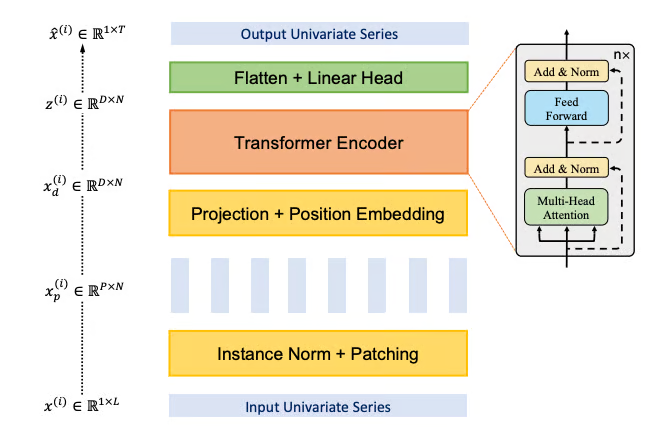
\includegraphics[width=0.78\textwidth]{figures/patchtst.png}
  \caption{PatchTST architecture for a univariate time series. The input sequence is normalized and divided into patches, embedded with positional information, processed by Transformer encoder blocks, and mapped to the output series by a linear head. Source: \cite{nie2023patchtst}.}
  \label{fig:patchtst-architecture}
\end{figure}

For a context of
length \(L\), patch length \(P\), and stride \(s\), the number of complete
patches is
\[
  N_p = 1 + \left\lfloor \frac{L-P}{s} \right\rfloor ,
\]
and the \(j\)-th patch is
\[
  p_j =
  [x_{1+(j-1)s}, \ldots, x_{1+(j-1)s+P-1}]
  \in \mathbb{R}^{P}.
\]
Each patch is projected into a \(d\)-dimensional token and combined with
positional information:
\[
  e_j = W_p p_j + b_p + r_j ,
\]
where \(W_p\) and \(b_p\) define the patch embedding and \(r_j\) encodes the
position of the patch inside the look-back window. The ordered token sequence
\([e_1,\ldots,e_{N_p}]\) is then processed by Transformer encoder blocks, whose
self-attention layers allow the representation of one patch to depend on other
patches in the context. A forecasting head maps the encoded representation to
the prediction horizon, for example through a direct multi-output projection
\[
  \widehat{Y} = W_o \operatorname{vec}(H) + b_o,
\]
where \(H\) denotes the encoded patch sequence.

Patching changes the granularity at which attention is applied. A token no
longer represents an individual sample; it represents a local temporal segment,
such as a short rise, plateau, oscillation, or recovery. This has two practical
effects. First, the embedding can preserve local shape information before the
global attention layers are applied. Second, the attention sequence length is
reduced from \(L\) to \(N_p\), lowering the cost of self-attention for the same
look-back window. The trade-off is that the patch length and stride become
important modeling choices: large or non-overlapping patches can smooth rapid
changes, while very short or highly overlapping patches reduce the computational
advantage and may behave closer to timestamp-level tokenization.

The second defining idea of PatchTST is channel independence. In a multivariate
series, each variable is treated as a separate univariate stream, with shared
embedding and Transformer weights across channels. This avoids forcing early
cross-channel mixing and improves scalability when many variables are present
\cite{nie2023patchtst}. In the signal-only setting of this thesis, there is only
one channel, so this design reduces to a purely univariate patch encoder. This
is consistent with the no-leakage and signal-only data policy: the model can
learn temporal structure in the recent signal history without receiving
additional covariates.

Practical implementations expose additional architectural and optimization
choices. The NeuralForecast implementation, for example, parameterizes the
forecast horizon and input size, the number of encoder layers and attention
heads, embedding size, patch length, stride, dropout, learnable positional
embeddings, residual attention, and reversible instance normalization
\cite{nixtlaPatchTSTDocs}. These options are not part of the task definition
itself; they control how the PatchTST family is instantiated and tuned. For
satellite fade nowcasting, the relevant motivation is that patch-level attention
can compare local fade patterns across the recent context while still producing
a direct forecast over the operational horizon.

\subsection{Foundation Time-Series Models}
\label{sec:background-chronos}

Foundation time-series models are pretrained on broad collections of time
series and then applied to new forecasting problems with little or no
task-specific training. Chronos is one such model family
\cite{ansari2024chronos}. It scales and quantizes real-valued time-series values
into discrete tokens and uses a language-model-style architecture to generate
future tokens autoregressively.

\begin{figure}[htbp]
  \centering
  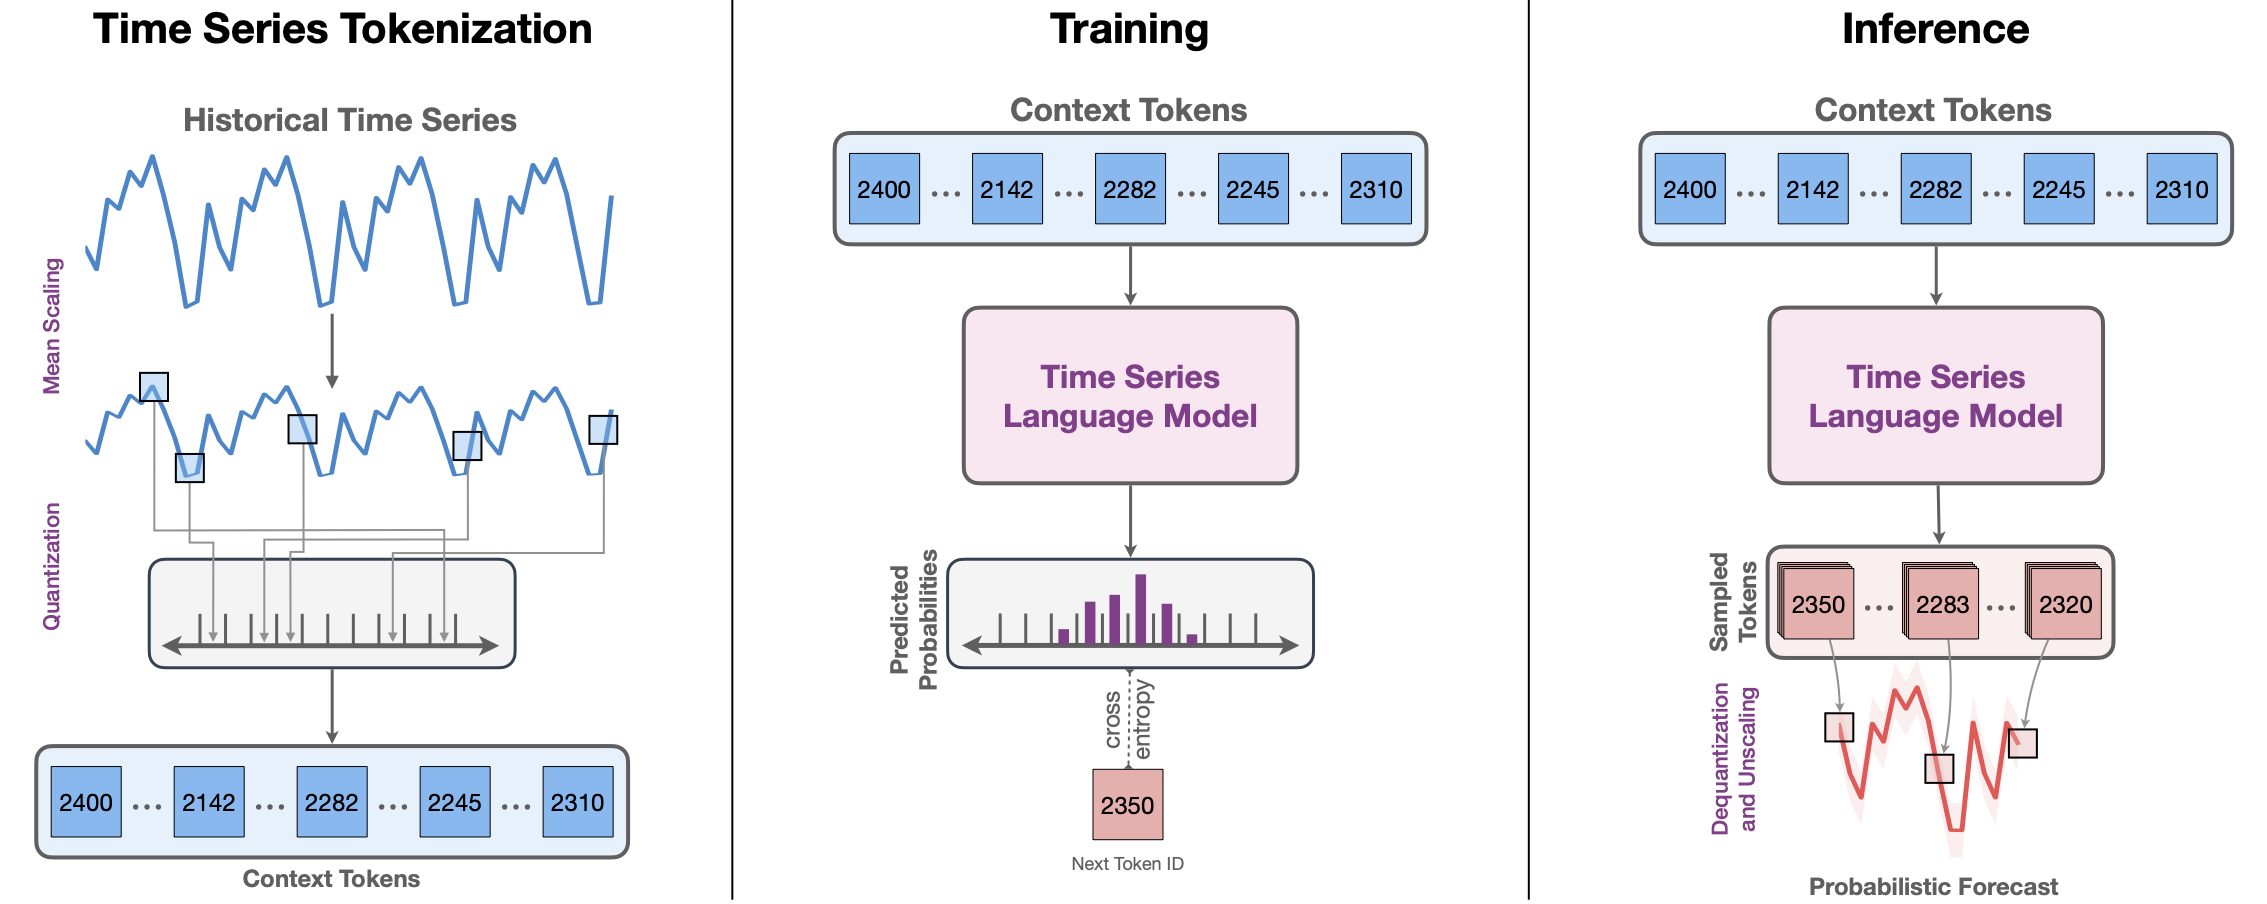
\includegraphics[width=0.95\textwidth]{figures/Chronos.png}
  \caption{High-level Chronos forecasting pipeline. The input time series is scaled and quantized into tokens, processed by a language-model architecture, and sampled autoregressively before being mapped back to numerical trajectories. Multiple sampled trajectories define a predictive distribution. Source: \cite{ansari2024chronos}.}
  \label{fig:chronos-overview}
\end{figure}

In zero-shot forecasting, a pretrained model receives only the past context from
the target series and produces a predictive distribution over future
trajectories:
\[
  p(\widehat{Y}_i \mid X_i).
\]
If multiple forecast samples are generated, a deterministic forecast can be
obtained by taking a statistic such as the median at each horizon. The main
advantage is that no project-specific parameter fitting is required. The main
limitation is domain transfer: the sampling cadence, scale, noise level, and
event structure of a satellite fade signal may differ from the data distribution
seen during pretraining.


\subsection{Temporal Convolutional Networks}
\label{sec:background-tcn}

Temporal convolutional networks use one-dimensional convolutions over ordered
sequences. A temporal convolution applies the same local filter at different
positions in the context, so the model can detect repeated patterns regardless
of where they occur inside the look-back window. This parameter sharing gives a
different inductive bias from lag-based trees, where each lag is a separate
feature, and from recurrent networks, where a hidden state is updated
sequentially.

Let \(x_t\in\mathbb{R}^{C_{\mathrm{in}}}\) be the input vector at sequence
position \(t\). A causal convolution with kernel size \(K\), dilation \(d\), and
output channel \(r\) can be written as
\[
  y_{t,r}
  =
  b_r
  +
  \sum_{c=1}^{C_{\mathrm{in}}}
  \sum_{a=0}^{K-1}
  W_{a,c,r}\,x_{t-ad,c}.
\]
The index \(t-ad\) is never greater than \(t\). The representation at position
\(t\) therefore depends only on current and past samples, which is the key
causality requirement for online nowcasting. In practice, causal convolution is
implemented with left padding or by trimming the output so that future samples
are never included in the receptive field.

The dilation factor spaces the filter taps apart. With \(d=1\), the convolution
uses adjacent samples \((x_t,x_{t-1},\ldots)\). With \(d=2\), it uses every
second sample \((x_t,x_{t-2},\ldots)\), and so on. Dilated causal convolutions
were popularized in sequence generation models such as WaveNet
\cite{oord2016wavenet}. Their advantage is that the receptive field can grow
rapidly without requiring very large kernels or very deep recurrent unrolling.

The receptive field is the part of the past that can influence an output. For a
stack of dilated convolutional layers with kernel sizes \(K_\ell\) and dilations
\(d_\ell\), assuming unit stride, the receptive field length is
\[
  R
  =
  1 + \sum_{\ell} (K_\ell-1)d_\ell .
\]
If a TCN block contains two convolutions with a common kernel size \(K\), and the
blocks use exponentially increasing dilations \(d_b=2^b\) for
\(b=0,\ldots,B-1\), the receptive field becomes
\[
  R
  =
  1 + 2(K-1)\sum_{b=0}^{B-1}2^b
  =
  1 + 2(K-1)(2^B-1).
\]
This formula makes an important modeling constraint explicit: a TCN can use
only the history covered by its receptive field. If \(R<L\), the earliest part
of a length-\(L\) context cannot affect the final output. If \(R\) is much larger
than the context, part of the nominal receptive field is filled by padding
rather than observed data.

A standard TCN is built from residual temporal blocks
\cite{bai2018tcn}. A block receives a sequence representation
\(H^{(b-1)}\in\mathbb{R}^{L\times C_b}\), applies causal dilated convolutions,
nonlinearities, normalization, and dropout, and adds the result back to the
input:
\[
  H^{(b)}
  =
  H^{(b-1)} + f_b(H^{(b-1)}).
\]
When the number of channels changes, a \(1\times 1\) convolution can project the
residual path to the correct dimension before the addition. The residual
connection helps optimization because each block learns a correction to the
previous representation instead of having to relearn the entire transformation.
Dropout and weight normalization are commonly used to stabilize training and
reduce overfitting in stacked convolutional sequence models.

\begin{figure}[htbp]
  \centering
  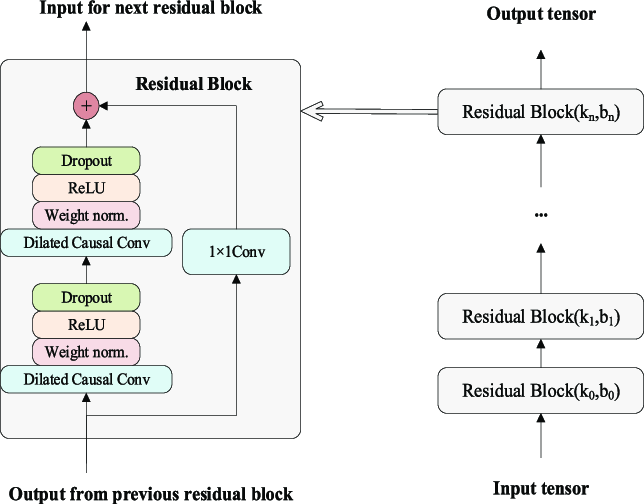
\includegraphics[width=0.72\textwidth]{figures/Architecture-of-temporal-convolutional-neural-networks-TCNs.png}
  \caption{Example architecture of a temporal convolutional network. Temporal convolutional blocks combine one-dimensional convolutions, nonlinear transformations, and residual connections to build sequence representations over a finite receptive field. Source: \cite{zhang2022attentionTcnRnn}.}
  \label{fig:tcn-architecture}
\end{figure}

For a sequence-level prediction, the final temporal representation must be
converted into a fixed-dimensional vector. Common choices include using the last
causal position, applying average or maximum pooling over time, or concatenating
several pooled summaries. The last-position representation is the most directly
causal for a decision at the end of the context, while temporal pooling can make
the model more sensitive to patterns that occurred anywhere in the look-back
window. For pointwise sequence outputs, such as a hazard at each future time bin
in a discrete-time survival model, the convolutional representation can instead
be mapped to a vector of horizon-specific logits.

TCNs occupy an intermediate position between recurrent and attention-based
models. Like GRUs, they can be made causal and are well suited to online
prediction. Unlike GRUs, they process all positions in parallel during training
and do not compress the entire past through a single recurrent state. Like
Transformers, they support parallel computation over the sequence, but their
dependency pattern is local and controlled by the receptive field rather than by
global self-attention. This makes them attractive when the relevant information
is expected to lie in local temporal shapes, slopes, threshold crossings, and
short persistence patterns. Their main limitation is that long-range dependence
must be covered deliberately through the choice of kernel size, dilation
schedule, and number of blocks; otherwise, distant samples are simply outside
the model's effective view.

In satellite fade nowcasting, this inductive bias is useful because many
operational cues are local but not instantaneous. A single sample above a
threshold may be ambiguous, whereas a short pattern of rising signal values,
oscillation near the threshold, or sustained exceedance can indicate a different
event regime. A causal TCN can learn filters for these patterns and combine
them across multiple temporal scales while preserving the no-leakage constraint.
This is why TCNs are suitable both for event classification and for
discrete-time hazard prediction, where the model must summarize recent history
before estimating the probability of future persistence or recovery.


\subsection{Shapelet-Based Time-Series Modeling}
\label{sec:background-shapelets}

A time-series shapelet is a short subsequence whose presence, absence, or
distance to a larger series is informative for prediction. Shapelets were
introduced as discriminative subsequences for interpretable time-series data
mining \cite{ye2009shapelets}. Shapelet transformations then made it possible
to use distances to selected shapelets as features for downstream classifiers
\cite{hills2014shapeletTransform}.

\begin{figure}[htbp]
  \centering
  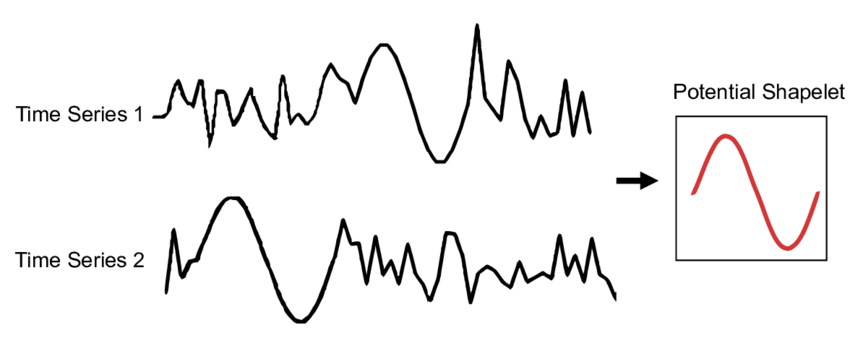
\includegraphics[width=0.85\textwidth]{figures/Time-series-shapelets.png}
  \caption{Illustration of time-series shapelets as local subsequences that are informative for distinguishing temporal patterns. Source: \cite{arul2020shapeletTransform}.}
  \label{fig:time-series-shapelets}
\end{figure}

Given a shapelet \(w\in\mathbb{R}^{\ell}\) and a context
\(x\in\mathbb{R}^{L}\), a standard squared-distance response is
\[
  d(x,w)
  =
  \min_{a=1,\ldots,L-\ell+1}
  \sum_{r=1}^{\ell}
  \left(x_{a+r-1}-w_r\right)^2 .
\]
The minimum over positions makes the feature approximately phase independent:
the pattern may appear early or late in the context and still produce a small
distance. This is useful for fade-related modeling because rapid rises,
temporary plateaus, partial recoveries, or oscillations around a threshold can
be informative even when they are not perfectly aligned across events.

The original shapelet approach searched over candidate subsequences and
selected discriminative patterns. Learnable shapelets instead treat the patterns
as differentiable model parameters optimized jointly with the prediction head
\cite{grabocka2014learning}. Multiscale learnable shapelets extend this idea by
using several shapelet lengths, allowing the model to represent both short
local transitions and longer local persistence patterns.


\subsection{Survival Analysis for Time-to-Recovery Modeling}
\label{sec:background-survival}

Survival analysis studies time-to-event outcomes in the presence of censoring.
Classical foundations include the Kaplan-Meier estimator for incomplete
observations \cite{kaplan1958nonparametric} and Cox regression models for
life-table data \cite{cox1972regression}. Let \(T\) be the true event time and
\(C\) the censoring time. The censoring time is the last time up to which the
sample can be followed before observation stops or before the event status
becomes unobservable. In this thesis, for example, a fade recovery is censored
when the acquisition segment ends before the end of the ongoing fade can be
seen. The observed time is
\[
  Y = \min(T,C),
\]
and the event indicator is
\[
  \Delta = \mathbb{1}[T \le C].
\]
If \(\Delta=0\), the event has not been observed by time \(Y\), so the valid
statement is that \(T>Y\). This is right censoring.

\begin{figure}[htbp]
  \centering
  \resizebox{\textwidth}{!}{%
  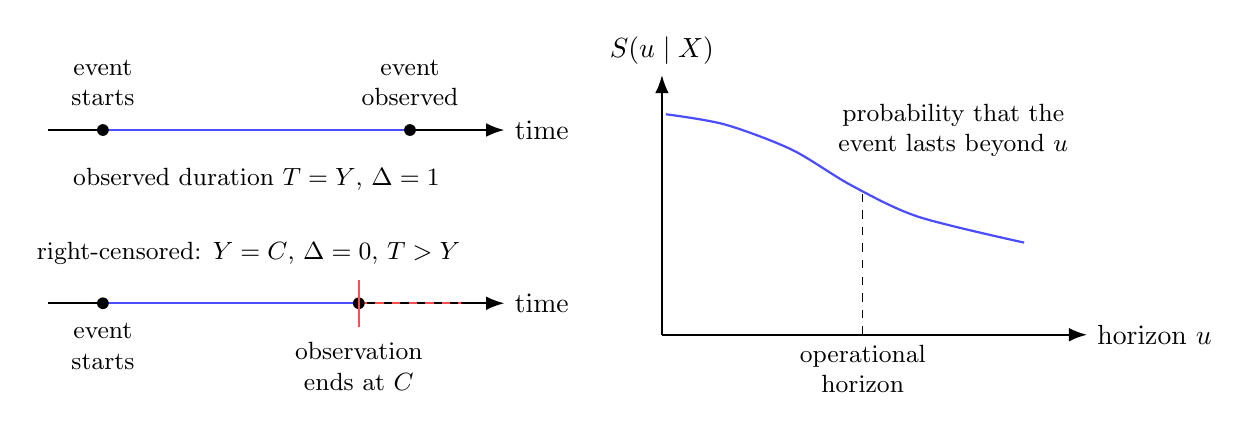
\begin{tikzpicture}[
      >=Latex,
      timeline/.style={thick, ->},
      event/.style={thick, blue!70},
      censored/.style={thick, red!70, dashed},
      marker/.style={circle, fill=black, inner sep=1.5pt},
      curve/.style={thick, blue!70},
      axis/.style={thick, ->},
      note/.style={align=center, font=\small}
    ]

    % Observed time-to-event example.
    \draw[timeline] (-6.6, 1.45) -- (-0.8, 1.45) node[right] {time};
    \draw[event] (-5.9, 1.45) -- (-2.0, 1.45);
    \node[marker] at (-5.9, 1.45) {};
    \node[marker] at (-2.0, 1.45) {};
    \node[note] at (-5.9, 2.05) {event\\starts};
    \node[note] at (-2.0, 2.05) {event\\observed};
    \node[note] at (-3.95, 0.82) {observed duration \(T=Y\), \(\Delta=1\)};

    % Right-censored example.
    \draw[timeline] (-6.6, -0.75) -- (-0.8, -0.75) node[right] {time};
    \draw[event] (-5.9, -0.75) -- (-2.65, -0.75);
    \draw[censored] (-2.65, -0.75) -- (-1.35, -0.75);
    \node[marker] at (-5.9, -0.75) {};
    \node[marker] at (-2.65, -0.75) {};
    \draw[red!70, thick] (-2.65, -1.05) -- (-2.65, -0.45);
    \node[note] at (-5.9, -1.3) {event\\starts};
    \node[note] at (-2.65, -1.55) {observation\\ends at \(C\)};
    \node[note] at (-4.05, -0.12) {right-censored: \(Y=C\), \(\Delta=0\), \(T>Y\)};

    % Survival curve.
    \draw[axis] (1.2, -1.15) -- (1.2, 2.15) node[above] {\(S(u\mid X)\)};
    \draw[axis] (1.2, -1.15) -- (6.6, -1.15) node[right] {horizon \(u\)};
    \draw[curve] plot[smooth] coordinates {
      (1.25,1.65) (2.0,1.52) (2.85,1.2) (3.6,0.75) (4.45,0.35) (5.8,0.02)
    };
    \draw[dashed] (3.75, -1.15) -- (3.75, 0.68);
    \node[note] at (3.75, -1.58) {operational\\horizon};
    \node[note] at (4.9, 1.45) {probability that the\\event lasts beyond \(u\)};
  \end{tikzpicture}
  }
  \caption{Basic survival-analysis quantities. Observed samples have a known event time, while right-censored samples are only known to survive beyond the last observable time. The survival curve maps each future horizon to the probability that the event has not yet ended.}
  \label{fig:survival-analysis-concepts}
\end{figure}

The survival function is
\[
  S(u \mid X) = P(T > u \mid X),
\]
which gives the probability that the event time exceeds horizon \(u\)
given the available input \(X\). In a satellite fade setting, the event of interest can be
interpreted as recovery from an ongoing fade rather than failure or death. This
makes survival analysis suitable for residual-duration questions, because a
survival curve can answer whether the current event is likely to last beyond an
operational horizon.

\subsubsection{Accelerated Failure Time Models and XGBoost-AFT}

Accelerated failure time (AFT) models are a parametric alternative to
proportional-hazards models. Instead of modeling the hazard ratio directly,
they model the logarithm of the event time as a location model
\cite{keiding2015survival,barnwal2022xgboostAft}:
\[
  \log T_i = \mu(X_i) + \tau \epsilon_i ,
\]
where \(X_i\) is the available input for sample \(i\), \(\mu(X_i)\) is a
location term, \(\tau>0\) is a scale parameter, and \(\epsilon_i\) follows a
chosen distribution such as normal, logistic, or extreme value. In a classical
linear AFT model, \(\mu(X_i)=\beta^\top X_i\). A positive change in
\(\mu(X_i)\) multiplies the typical event time by a factor on the original
time scale, which motivates the term ``accelerated'' failure time.

The AFT formulation is useful for censored duration targets because each sample
can be represented by lower and upper bounds on its event time. If the recovery
time is observed exactly, both bounds correspond to the observed duration,
\(L_i=U_i=T_i\). If the sample is right-censored at the end of the observable
segment, the only valid statement is \(T_i>C_i\), which can be encoded as
\(L_i=C_i\) and \(U_i=\infty\). More generally, the likelihood contribution of
an interval-censored observation is the model probability that the event time
lies inside the interval:
\[
  P(L_i < T_i \le U_i \mid X_i)
  =
  F_{\epsilon}
  \left(
    \frac{\log U_i - \mu(X_i)}{\tau}
  \right)
  -
  F_{\epsilon}
  \left(
    \frac{\log L_i - \mu(X_i)}{\tau}
  \right),
\]
with the appropriate density limit used for exact observations and with the
upper cumulative term equal to one when \(U_i=\infty\). The negative
log-likelihood derived from these terms trains the model without discarding
censored samples.

XGBoost-AFT keeps the same censored-label likelihood but replaces the linear
location term with a boosted tree ensemble:
\[
  \mu(X_i) = F(\phi_i) = \sum_{m=1}^{M} f_m(\phi_i),
\]
where \(\phi_i\) is the tabular representation of the available context
\cite{xgboostAftDocs,barnwal2022xgboostAft}. This is important for the present
thesis because the survival-persistence task uses past signal windows and
scalar summaries as input, while the target is a residual fade duration that
may be censored by the end of an acquisition segment. XGBoost-AFT can therefore
learn a nonlinear mapping from the current context to the location of the
log-duration distribution while still using both observed and right-censored
training samples.

Once \(\mu(X_i)\), the scale parameter, and the error distribution are fixed,
the model implies a full conditional survival curve:
\[
  S(u\mid X_i)
  =
  P(T_i>u\mid X_i)
  =
  1 -
  F_{\epsilon}
  \left(
    \frac{\log u - \mu(X_i)}{\tau}
  \right).
\]
Thus XGBoost-AFT does not output a binary switch by itself. It first defines a
distribution over the residual duration; an operational switch decision is then
obtained by evaluating the survival probability at a chosen horizon and applying
a configured probability threshold.

Discrete-time neural survival models partition time into ordered bins and
predict a hazard probability for each bin. If \(h_k(X)\) is the conditional
event probability in bin \(k\), then the discrete survival probability after
\(K\) bins is
\[
  S_K(X)
  =
  \prod_{k=1}^{K} \left(1-h_k(X)\right).
\]
Neural discrete-time survival models can be trained with likelihood terms for
both observed and censored samples \cite{gensheimer2019nnet}. When the hazard
model is implemented with a sequence architecture, the input representation can
still be restricted to the past context while the output retains a
time-to-event interpretation.

\section{Nowcasting Problem and Validation Principles}
\label{sec:background-nowcasting}

The model families described above provide different ways to represent temporal
information. Defining a prediction problem additionally requires specifying
when a prediction is issued, which observations are available at that time, and
which unknown outcome the prediction should describe. These choices establish
the nowcasting setting and determine what constitutes a meaningful evaluation.

\subsection{Prediction at the Current Time}

Nowcasting refers to very short-range prediction from the current and recent
state of a system. In meteorology, the World Meteorological Organization
describes nowcasting as detailed local forecasting from the present to a few
hours ahead using rapidly updated observations \cite{wmo2017nowcasting}.
The term is used here for signal-based estimates of the near-future evolution
or persistence of an ongoing satellite-link degradation, issued to support an
operational decision in the next few minutes.

At a decision time \(t_i\), the observed history supplies the information set
\(\mathcal{F}_i\), and the past context \(X_i\) is a finite representation of
that information. The target \(Y_i\) specifies the outcome to be estimated from
this information. It may concern future signal values, a remaining duration, or
an event property whose definitive label requires later observations. With model
parameters fixed for evaluation, the prediction \(z_i=f_\vartheta(X_i)\) must
be computable from information available at \(t_i\). The target can be
established retrospectively when the relevant future has been observed, or
represented as incomplete supervision when observation ends first.

The look-back duration and the prediction horizon have different roles. The
context specifies how much past information is supplied to the model; the
horizon specifies how far ahead an outcome is assessed. For a regularly sampled
forecast with interval \(\Delta\), the \(h\)-step horizon corresponds to
\(h\Delta\) units of elapsed time. A duration or survival model can instead
describe persistence over a broader range while still informing a decision at
a fixed short operational horizon. Thus, a common decision horizon does not
require every predictive task to have the same target representation.

The operational question in this thesis is whether the evolution or persistence
inferred at \(t_i\) justifies activating a backup communication link. Observing
that degradation is present does not by itself answer that question: the
unobserved continuation determines whether the interruption will be brief or
sustained. The predictive output therefore supplies evidence for a decision,
through an explicitly defined conversion rule. The satellite context is
developed in \cref{sec:background-satellite-operational}, and the alternative
targets and conversion rules are formalized in \cref{chap:task-formulations}.

\subsection{Temporal Generalization and Validation}
\label{sec:background-validation}

Evaluation must reflect the information constraints of this prediction problem.
Two distinct requirements arise: each input must respect its decision-time
boundary, and the evaluation data must test the intended form of generalization.
A past-only input is insufficient if the training and evaluation sets contain
near-duplicate windows from the same episode.

For example, a random split may place \(X_i\) in training and \(X_{i+1}\) in
testing even though they share \(L-1\) observations. Target horizons may overlap
as well. Such a split can primarily measure interpolation within already
represented episodes, whereas the operational question concerns performance on
episodes or acquisition periods that were not used to fit the model.

This does not imply that standard cross-validation is invalid for every time
series problem. Bergmeir et al. establish conditions under which it can be used
for autoregressive prediction, including uncorrelated model errors
\cite{bergmeir2018note}. Those conditions should not be assumed merely because a
time series has been stored as a table. Temporal dependence, distribution
changes, and repeated windows from the same physical episode motivate
chronological or event-grouped development splits. Holding out an entire source
dataset addresses the additional question of transfer to a different acquisition
record.

Training data are used to fit parameters. Validation data guide model and
hyperparameter selection, early stopping, and any learned decision threshold.
Test data assess the resulting fixed procedure. Transformations with fitted
parameters must follow the same separation. Changing a decision rule after
inspecting test performance makes that comparison exploratory rather than an
independent final evaluation. The concrete external-holdout construction and
experimental protocol are specified in
\cref{chap:data-reference-framework,chap:experimental-setup}.

\section{Satellite and Operational Background}
\label{sec:background-satellite-operational}

\subsection{Earth-Space Propagation and Fade Events}
\label{sec:background-earth-space-attenuation}

An Earth-space communication link is affected by deterministic link-budget terms
and by time-varying propagation impairments. The deterministic terms include
transmit power, antenna gains, free-space path loss, and receiver noise
characteristics. The time-varying terms include atmospheric gases, clouds, rain,
tropospheric scintillation, depolarization, and low-elevation effects. These
effects become increasingly important at high carrier frequencies. In Ku-, Ka-,
and V-band satellite systems, atmospheric attenuation is one of the main limits
to link availability and therefore a central design and operational concern
\cite{panagopoulos2004satellite,ippolito2017rainFadeMitigation}.

The International Telecommunication Union provides several recommendations for
Earth-space propagation engineering. Recommendation ITU-R P.618 gives methods
for propagation data and prediction in Earth-space telecommunication systems
\cite{iturP618}. Recommendation ITU-R P.837 provides precipitation statistics
used by propagation models \cite{iturP837}. Recommendation ITU-R P.1623 focuses
on fade dynamics, including fade duration and fade slope on Earth-space paths
\cite{iturP1623}, while Recommendation ITU-R P.1853 addresses synthesis of
tropospheric impairment time series \cite{iturP1853}. These documents are
important because they show that attenuation is not only a static exceedance
probability problem. Its temporal structure, including how long fades last and
how quickly they evolve, matters for systems that react dynamically.

Rain attenuation is especially relevant for short-term availability. Rain cells
can produce strong and localized signal degradation, and their movement through
the slant path causes attenuation to rise, fluctuate, and recover over time. A
classical example of dynamic rain-attenuation modeling is the stochastic model
of Maseng and Bakken \cite{maseng1981stochastic}. This thesis does not build a
physical rain model and does not use rain-rate measurements as inputs. The
propagation literature nevertheless motivates the modeling premise that recent
signal history contains information about the near-future state of the link,
while the useful information is local, noisy, and event dependent.

In the data representation used in this work, the measured column \(S_i\) is
treated as a signal or fade-level quantity. Larger values correspond to worse
link conditions. A fade region is therefore defined by an operational threshold
\[
  S_i \ge \theta .
\]
Real fade events are not perfectly smooth: the signal can cross below and above
the threshold several times during one physical degradation episode. Operational
event definitions therefore need persistence, grouping, or stable-recovery
rules rather than relying only on isolated threshold crossings.

\subsection{Fade Mitigation Techniques}

Satellite systems can respond to fading through several fade mitigation
techniques. Examples include static fade margins, uplink power control,
adaptive coding and modulation, bandwidth or data-rate adaptation, site
diversity, and switching traffic to an alternative path or backup link
\cite{panagopoulos2004satellite,ippolito2017rainFadeMitigation}. These
techniques have different physical and operational costs. Increasing transmit
power consumes power budget and may be limited by hardware or regulatory
constraints. Adaptive coding and modulation protects the link by lowering
spectral efficiency. Site diversity or backup-link switching consumes shared
network resources and can require non-negligible activation time.

Because mitigation has a cost, the operational objective is not to react to
every threshold crossing. A short isolated fade may be tolerable, while a fade
that is expected to persist for several minutes may justify early activation of
a backup resource. This turns attenuation monitoring into a short-term decision
problem: the system must use recent observations to decide whether the current
or imminent fade is persistent enough to justify action.

\subsection{Switch Decisions and Operational Metrics}
\label{sec:background-operational-evaluation}

The final operational decision considered in the thesis is binary: switch or do
not switch. Different predictive tasks may estimate different intermediate
quantities before that decision is made. A forecasting model estimates future
signal values, a duration model estimates persistence time, a classifier
estimates an event probability, and a survival model estimates a residual
duration curve. These outputs are not directly comparable until each is
converted into a binary switch sequence.

This separation between model output and switch rule is important. A model can
have a low native predictive loss but still produce poor operational behavior
if its errors occur near the threshold, if it triggers too many short switch
islands, or if it activates too late inside a fade. Conversely, a model with
moderate native error can be operationally useful if it makes reliable decisions
near the switch boundary.

For this reason, this thesis distinguishes between native predictive metrics and
operational switch metrics. Native metrics evaluate the intermediate quantity
predicted by a model. Switch metrics evaluate the binary decision sequence after
task-specific conversion and common post-processing.

For real-valued forecasting or duration regression, the main error measures are
mean absolute error and root mean squared error. Given targets \(y_i\) and
predictions \(\widehat{y}_i\), they are
\[
  \operatorname{MAE}
  =
  \frac{1}{N}
  \sum_{i=1}^{N}
  \left|\widehat{y}_i-y_i\right|,
\]
and
\[
  \operatorname{RMSE}
  =
  \sqrt{
  \frac{1}{N}
  \sum_{i=1}^{N}
  \left(\widehat{y}_i-y_i\right)^2
  } .
\]
MAE gives the average absolute error in the physical unit of the target. RMSE
penalizes large errors more strongly because the residuals are squared before
averaging. In multi-step forecasting, these quantities can also be computed by
horizon step, replacing the single target \(y_i\) with
\(y_{i,k}\), \(k=1,\ldots,h\).

For binary classification, let \(q_i\in[0,1]\) be the predicted probability and
\(y_i\in\{0,1\}\) the true class. A probability threshold converts \(q_i\) into a
class prediction. Precision, recall, and F1 are then defined from the confusion
counts
\[
\begin{aligned}
  TP &= \sum_i \mathbb{1}[\widehat{y}_i=1 \land y_i=1], &
  FP &= \sum_i \mathbb{1}[\widehat{y}_i=1 \land y_i=0], \\
  TN &= \sum_i \mathbb{1}[\widehat{y}_i=0 \land y_i=0], &
  FN &= \sum_i \mathbb{1}[\widehat{y}_i=0 \land y_i=1].
\end{aligned}
\]
The corresponding metrics are
\[
  \operatorname{Precision}=\frac{TP}{TP+FP},
  \qquad
  \operatorname{Recall}=\frac{TP}{TP+FN},
\]
and
\[
  F_1
  =
  \frac{
    2\,\operatorname{Precision}\,\operatorname{Recall}
  }{
    \operatorname{Precision}+\operatorname{Recall}
  } .
\]
The area under the receiver operating characteristic curve, AUROC, evaluates
the ranking of positive samples above negative samples across all possible
thresholds. The area under the precision-recall curve, AUPRC, evaluates the
precision-recall trade-off across thresholds and is often more informative when
the positive class is rare.

For survival models, the output is not a point estimate or a class probability
but a survival curve \(S(u\mid X)\). The negative log-likelihood measures how
much probability the model assigns to the observed time-to-event information.
For interval survival labels \([L_i,U_i]\), used for accelerated failure time
models, a generic contribution is
\[
  -\log P(L_i \le T_i \le U_i \mid X_i),
\]
with \(U_i=\infty\) for right-censored samples. In that case, the likelihood
term becomes the probability of surviving beyond the censoring lower bound.
Harrell's concordance index evaluates ranking quality: it is the fraction of
comparable sample pairs for which the model assigns shorter predicted survival
to the sample with the earlier observed event time. A value of \(0.5\) is
approximately random ranking, while a value near \(1\) indicates strong
ordering.

The Brier score evaluates the calibration and discrimination of survival
probabilities at a fixed horizon \(u\). In its simplest uncensored form, it is
\[
  \operatorname{BS}(u)
  =
  \frac{1}{N}
  \sum_{i=1}^{N}
  \left(
    \mathbb{1}[T_i>u] - \widehat{S}(u\mid X_i)
  \right)^2 .
\]
With censoring, inverse-probability-of-censoring weighting is commonly used to
avoid treating censored event status as known. The integrated Brier score
aggregates the horizon-wise Brier score over a range of horizons,
\[
  \operatorname{IBS}
  =
  \frac{1}{u_{\max}-u_{\min}}
  \int_{u_{\min}}^{u_{\max}} \operatorname{BS}(u)\,du,
\]
or the corresponding discrete average over evaluated time bins.

Operational switch metrics reuse the same confusion-count logic, but the
positive class is now a switch decision rather than a native task label. Let
\(m_i\in\{0,1\}\) denote the post-processed model switch and
\(p_i\in\{0,1\}\) the aligned Perfect Switch reference. The switch-level
confusion counts are
\[
\begin{aligned}
  TP &= \sum_i \mathbb{1}[m_i=1 \land p_i=1], &
  FP &= \sum_i \mathbb{1}[m_i=1 \land p_i=0], \\
  TN &= \sum_i \mathbb{1}[m_i=0 \land p_i=0], &
  FN &= \sum_i \mathbb{1}[m_i=0 \land p_i=1].
\end{aligned}
\]
In addition to precision, recall, and F1, switch evaluation reports
intersection over union,
\[
  \operatorname{IoU}=\frac{TP}{TP+FP+FN},
\]
balanced accuracy,
\[
  \operatorname{BalancedAccuracy}
  =
  \frac{1}{2}
  \left(
    \frac{TP}{TP+FN}
    +
    \frac{TN}{TN+FP}
  \right),
\]
false positive rate and false negative rate,
\[
  \operatorname{FPR}=\frac{FP}{FP+TN},
  \qquad
  \operatorname{FNR}=\frac{FN}{FN+TP}.
\]
Undefined divisions are handled explicitly rather than silently converted to
optimistic values.

Pointwise switch metrics are complemented by duration and event-level behavior
metrics. Active duration counts how many samples the model keeps the switch
active,
\[
  D_m=\sum_i m_i,
\]
or \(D_m\Delta t\) in seconds when the sampling time is \(\Delta t\). The
Perfect Switch duration is \(D_p=\sum_i p_i\), and the outage-mask duration is
the number of samples for which the observed signal itself is above the
threshold. The number of model switch islands is
\[
  N_m =
  \sum_i
  \mathbb{1}\left[m_i=1 \land (i=1 \lor m_{i-1}=0)\right].
\]
Detected events count Perfect Switch events that overlap at least one model
switch island. Missed events count Perfect Switch events without model overlap.
False switch events count model switch islands that do not overlap a Perfect
Switch event. When the onset of both the reference and the model switch island
is available, onset delay measures the model onset time relative to the
reference onset. Duration similarity is reported as
\[
  100\,\frac{D_p-|D_m-D_p|}{D_p}.
\]
These metrics connect statistical modeling to the practical behavior of a
fade mitigation system: they quantify not only whether the model is correct at
individual timestamps, but also whether it activates too long, misses events,
fragments one event into many switch islands, or reacts too late.

\chapter{Data and Reference Decision Framework}
\label{chap:data-reference-framework}

The operational problem addressed in this thesis starts from a stream of
timestamped satellite signal measurements and asks whether the link condition
justifies activating a backup resource. Before any model can be trained, this
problem requires a precise data and decision framework: the raw files must be
converted into a common signal representation, invalid observations and gaps
must be handled consistently, continuous acquisition segments must be defined,
and the reference switch sequence must be constructed from explicit rules.

This chapter defines that framework. Its purpose is not only to prepare data
for modeling, but to fix the operational meaning of the quantities evaluated
later in the thesis. The same data layer determines what counts as an available
observation at prediction time, how heterogeneous sources are reduced to the
signal-only schema, how candidate fade periods are identified, and how model
outputs are compared against a common Perfect Switch reference. The experimental
split and validation protocol then follow from this framework, because model
comparisons are only meaningful when they share the same cleaned data,
timestamp grid, reference decision, and post-processing policy.

\section{Data Preparation Pipeline Overview}
\label{sec:data-preparation-pipeline-overview}

The complete preparation flow is summarized in
\cref{fig:data-preparation-pipeline}. The diagram is intended as a map for the
rest of the chapter: each block is introduced here once, and the following
sections describe the corresponding assumptions and implementation choices in
detail.

\begin{figure}[p]
\centering
\vspace*{-0.35cm}

\resizebox{0.98\textwidth}{!}{%
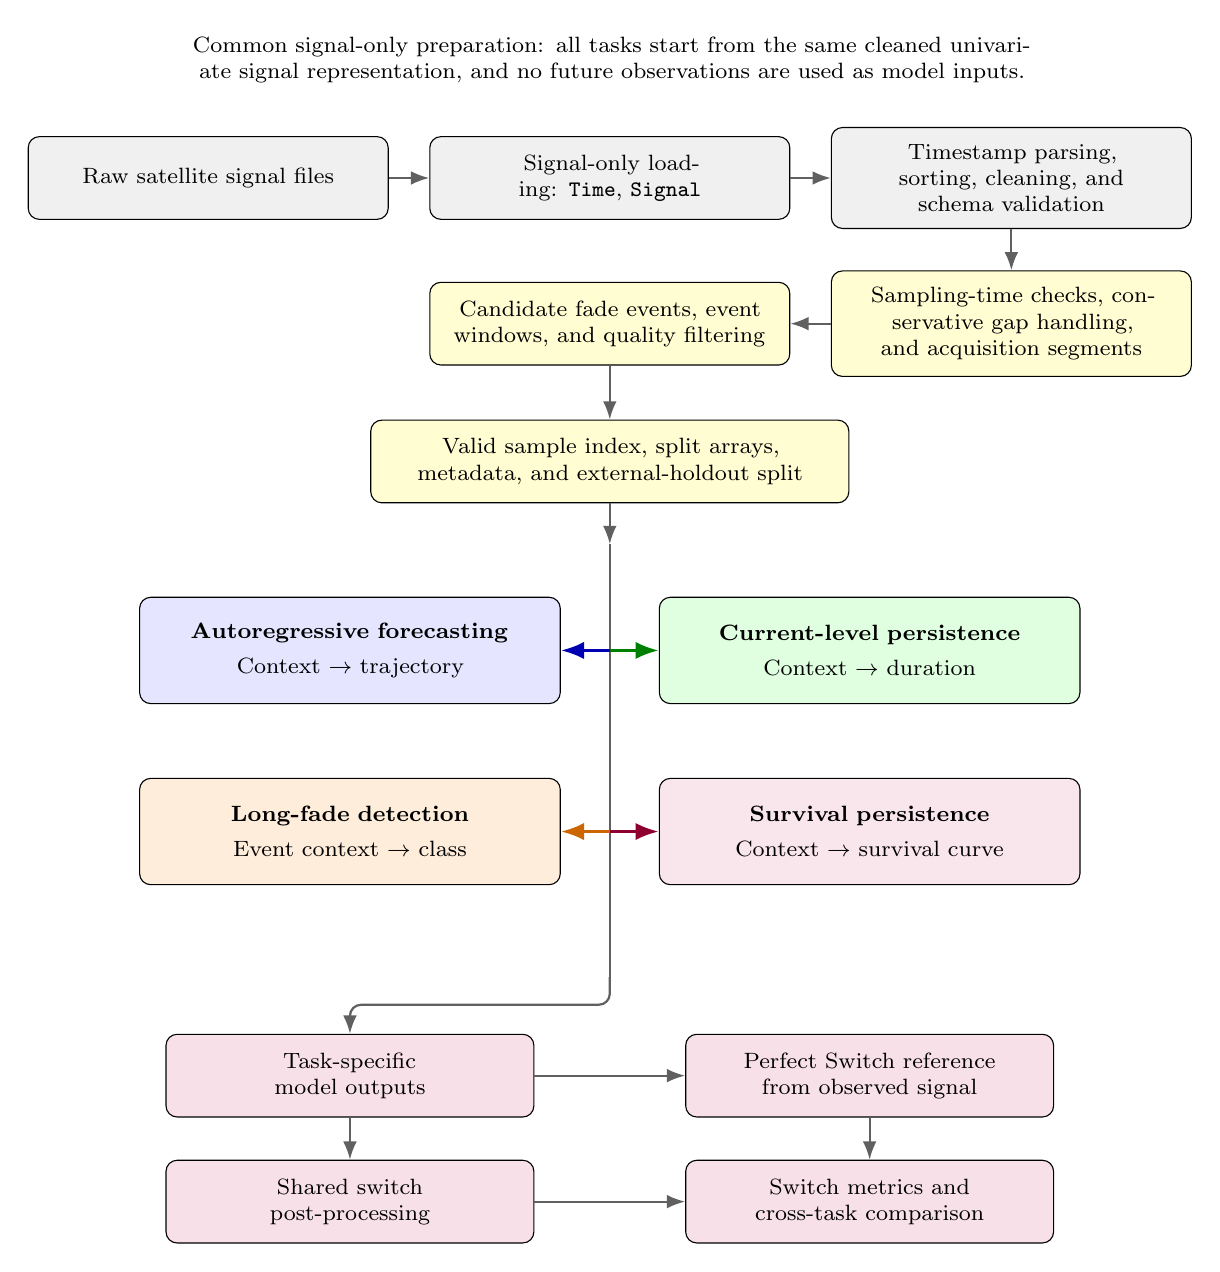
\begin{tikzpicture}[
    >=Latex,
    common/.style={
        draw,
        rounded corners,
        fill=gray!12,
        align=center,
        text width=4.15cm,
        minimum height=1.05cm,
        inner sep=6pt,
        font=\footnotesize
    },
    prep/.style={
        draw,
        rounded corners,
        fill=yellow!18,
        align=center,
        text width=4.15cm,
        minimum height=1.05cm,
        inner sep=6pt,
        font=\footnotesize
    },
    lane/.style={
        draw,
        rounded corners,
        align=center,
        text width=4.85cm,
        minimum height=1.35cm,
        inner sep=7pt,
        font=\footnotesize
    },
    eval/.style={
        draw,
        rounded corners,
        fill=purple!12,
        align=center,
        text width=4.25cm,
        minimum height=1.05cm,
        inner sep=6pt,
        font=\footnotesize
    },
    arrow/.style={->, thick, gray!75!black},
    ararrow/.style={->, very thick, blue!70!black},
    clparrow/.style={->, very thick, green!50!black},
    lfdarrow/.style={->, very thick, orange!80!black},
    sparrow/.style={->, very thick, purple!75!black},
    note/.style={align=center, font=\footnotesize}
]

% ============================================================
% Introductory note
% ============================================================

\node[
    note,
    text width=12.5cm
] at (5.10,0.65)
{
Common signal-only preparation: all tasks start from the same cleaned
univariate signal representation, and no future observations are used
as model inputs.
};

% ============================================================
% Common preprocessing
% ============================================================

\node[common] (raw) at (0.00,-0.85)
    {Raw satellite signal files};

\node[common] (load) at (5.10,-0.85)
    {Signal-only loading: \texttt{Time}, \texttt{Signal}};

\node[common] (clean) at (10.20,-0.85)
    {Timestamp parsing, sorting, cleaning, and schema validation};

% Slightly raised preprocessing row
\node[prep] (segments) at (10.20,-2.70)
    {Sampling-time checks, conservative gap handling,
     and acquisition segments};

\node[prep] (events) at (5.10,-2.70)
    {Candidate fade events, event windows, and quality filtering};

% Slightly lowered to create more separation
\node[
    prep,
    text width=5.65cm
] (split) at (5.10,-4.45)
    {Valid sample index, split arrays, metadata,
     and external-holdout split};

% Common pipeline arrows

\draw[arrow] (raw) -- (load);
\draw[arrow] (load) -- (clean);
\draw[arrow] (clean.south) -- (segments.north);
\draw[arrow] (segments.west) -- (events.east);
\draw[arrow] (events.south) -- (split.north);

% ============================================================
% Task branching
% ============================================================

% Slightly lowered together with split
\coordinate (branch) at (5.10,-5.50);

\draw[arrow] (split.south) -- (branch);

% ============================================================
% Task-specific blocks
% ============================================================

\node[
    lane,
    fill=blue!10
] (ar) at (1.80,-6.85)
{
\textbf{Autoregressive forecasting}\\[3pt]
Context \(\rightarrow\) trajectory
};

\node[
    lane,
    fill=green!12
] (clp) at (8.40,-6.85)
{
\textbf{Current-level persistence}\\[3pt]
Context \(\rightarrow\) duration
};

\node[
    lane,
    fill=orange!14
] (lfd) at (1.80,-9.15)
{
\textbf{Long-fade detection}\\[3pt]
Event context \(\rightarrow\) class
};

\node[
    lane,
    fill=purple!10
] (sp) at (8.40,-9.15)
{
\textbf{Survival persistence}\\[3pt]
Context \(\rightarrow\) survival curve
};

% ============================================================
% Central branch
% ============================================================

\coordinate (branchbottom) at (5.10,-11.00);

\draw[
    thick,
    gray!75!black
] (branch) -- (branchbottom);

% Horizontal task arrows

\draw[ararrow]
    (5.10,-6.85) -- (ar.east);

\draw[clparrow]
    (5.10,-6.85) -- (clp.west);

\draw[lfdarrow]
    (5.10,-9.15) -- (lfd.east);

\draw[sparrow]
    (5.10,-9.15) -- (sp.west);

% ============================================================
% Shared reference / evaluation
% ============================================================

\node[eval] (derived) at (1.80,-12.25)
{
Task-specific\\
model outputs
};

\node[eval] (perfect) at (8.40,-12.25)
{
Perfect Switch reference\\
from observed signal
};

\node[eval] (post) at (1.80,-13.85)
{
Shared switch\\
post-processing
};

\node[eval] (metrics) at (8.40,-13.85)
{
Switch metrics and\\
cross-task comparison
};

% ============================================================
% Evaluation arrows
% ============================================================

\draw[arrow, rounded corners=4pt]
    (branchbottom)
    -- ++(0,-0.35)
    -| (derived.north);

\draw[arrow]
    (derived.east) -- (perfect.west);

\draw[arrow]
    (derived.south) -- (post.north);

\draw[arrow]
    (perfect.south) -- (metrics.north);

\draw[arrow]
    (post.east) -- (metrics.west);

\end{tikzpicture}%
}

\caption{Overview of the signal-only data preparation and reference-decision
pipeline. Gray and yellow blocks are shared preprocessing steps; colored
blocks are task-specific dataset targets and downstream switch-evaluation
inputs.}

\label{fig:data-preparation-pipeline}
\end{figure}


The key point is that the pipeline is shared up to the point where each
modeling task requires a different target. Autoregressive forecasting needs
past-future signal windows, current-level persistence needs residual duration
relative to the current signal level, long-fade detection needs a grouped-event
class label, and survival persistence needs observed or right-censored
remaining event durations. The raw data cleaning, segment boundaries, external
holdout policy, and switch reference construction remain common, so differences
in the results can be attributed to the task formulation and model family
rather than to incompatible preprocessing.

\section{Available Signal Datasets}

The project uses a collection of satellite fade and beacon signal files
associated with the Fucino ground segment in Italy and with GX4/GX5 satellite
links \cite{telespazio_fucino,satbeams_gx4,satbeams_gx5}. The files were made
available for this thesis as project data rather than as a public benchmark
dataset. They cover different sources and acquisition periods. Each file
contains a sequence of timestamped observations of the link signal or
attenuation level, but the raw format is not homogeneous across sources. Some
files include explicit column headers, while others are plain delimited files
without column names. Some files contain only timestamp and signal columns,
whereas a small subset includes additional environmental columns. The first
requirement of the data layer is therefore to map these heterogeneous files
into a common representation before any task-specific dataset is built.

The raw inventory used in the final experiments contains eight loaded signal
datasets. Their time coverage ranges from several weeks to several months, with
the earliest acquisition starting in July 2020 and the latest ending in July
2021. \Cref{tab:raw-dataset-inventory} summarizes the loaded files at the level
needed for the experimental protocol.

\begin{table}[htbp]
  \centering
  \caption{Raw signal datasets used in the project inventory. Row counts refer
  to valid rows after the common loading and validation stage.}
  \label{tab:raw-dataset-inventory}
  \begin{tabular}{lrr}
    \toprule
    Dataset & Valid rows & Duration (hours) \\
    \midrule
    \texttt{uplink\_beacon\_data\_fucino\_GX4.csv} & 481715 & 4081.5 \\
    \texttt{dati\_meteo\_beacon.csv} & 484031 & 4081.5 \\
    \texttt{fc-uplink-fade.csv} & 378191 & 3218.0 \\
    \texttt{fc-downlink-fade.csv} & 380566 & 3215.8 \\
    \texttt{UPLINK-FADE\_Fucino\_GX4\_AprJun2021.csv} & 259992 & 2171.7 \\
    \texttt{UPLINK-FADE\_Fucino\_GX5\_AprJun2021.csv} & 256519 & 2161.0 \\
    \texttt{DOWNLINK-FADE\_Fucino\_GX4\_MarJun2021.csv} & 338281 & 2826.0 \\
    \texttt{DOWNLINK-FADE\_Fucino\_GX5\_AprJun2021.csv} & 256519 & 2161.0 \\
    \bottomrule
  \end{tabular}
\end{table}

All datasets used in this work are associated with measurements from the
Fucino ground segment in Italy. Fucino is one of Telespazio's main space
centres and teleports \cite{telespazio_fucino}. The satellite identifiers in
the file names refer to GX4 and GX5, corresponding to the Inmarsat Global
Xpress spacecraft Inmarsat GX4, catalogued as NORAD 42698, and Inmarsat GX5,
catalogued as NORAD 44801 \cite{satbeams_gx4,satbeams_gx5}. Viasat completed
its acquisition of Inmarsat in 2023, so these spacecraft belong to the current
Viasat/Inmarsat provider context \cite{viasat_inmarsat_acquisition}. The
historical Inmarsat GX names are nevertheless retained in this thesis because
they are the identifiers used in the raw files and in public satellite
catalogues.

Within this context, several files are also related by link direction. In the
dataset names, \emph{uplink} denotes the ground-to-satellite propagation path,
while \emph{downlink} denotes the satellite-to-ground propagation path. Thus,
uplink and downlink files can be interpreted as physically paired measurements
or derived fade series for opposite directions of the same broader
communication link, especially when they refer to the same site and payload
identifier. In this thesis, however, these files are not combined into a
multivariate paired representation. Each file is treated as an independent
univariate signal series, because the final modeling policy requires the same
single input variable, \texttt{Signal}, to be available for every dataset.

The datasets differ not only in their acquisition period, but also in their
maximum observed signal excursions and in the amount of invalid or missing
source rows. They also differ in the availability of auxiliary variables.
\Cref{tab:ignored-source-columns} reports the files whose raw format contains
more than the timestamp and signal fields used by the models.

\begin{table}[htbp]
  \centering
  \caption{Additional source columns found in the raw files and ignored by the
  signal-only data policy.}
  \label{tab:ignored-source-columns}
  \begin{tabular}{lp{8.5cm}}
    \toprule
    Dataset & Ignored source columns \\
    \midrule
    uplink beacon GX4
      & \texttt{Temperature}, \texttt{Pressure}, \texttt{Humidity} \\
    meteo beacon
      & \texttt{airt\_bt}, \texttt{pres\_bt}, \texttt{relh\_bt}, \texttt{temp\_bt} \\
    fc-uplink fade
      & third trailing column, empty in the inspected rows \\
    fc-downlink fade
      & third trailing column, empty in the inspected rows \\
    \bottomrule
  \end{tabular}
\end{table}

The environmental columns would be potentially useful in a broader
multivariate nowcasting study, since atmospheric conditions can affect
attenuation dynamics. They are not used here because they are not available in a
consistent form across all datasets. Including them would force the experiments
to either discard most datasets or compare models trained with different input
information. By contrast, several of the Fucino 2021 files contain exactly two
columns and are loaded through positional column selection. This variability
motivates the strict loading policy described in the next section: downstream
models should not depend on source-specific formatting decisions.

The final experimental protocol treats \texttt{fc-uplink-fade.csv} as an
external holdout. This file is included in the project inventory and in the
final processed datasets, but it is reserved for test evaluation. All remaining
datasets form the development pool used for training and validation. Exact
supervised sample counts are reported with the experimental setup, because they
depend on the task-specific target and validity rules.

\section{Signal-Only Policy}

All models in this thesis follow a strict signal-only policy. After loading and
validation, every dataset is standardized to exactly two columns:

\begin{center}
\texttt{Time}, \texttt{Signal}.
\end{center}

The \texttt{Time} column identifies when the observation was acquired. It is
used for chronological ordering, gap detection, elapsed-duration computation,
and splitting into train, validation, and test sets. It is not used directly as
a model input.
The \texttt{Signal} column is the only measured variable made available to the
models. In the raw files, this quantity represents the signal or fade level
used to describe the link degradation. The exact source formatting may differ,
but after the common loading step all downstream tasks operate on the same
semantic object: a univariate time series of signal values.

This policy is deliberately restrictive. Some raw files contain environmental
measurements, such as temperature, pressure, or humidity, and these variables
could plausibly improve attenuation nowcasting in a dedicated multivariate
study. They are excluded here because they are not available consistently
across the full dataset collection. If such variables were used, the
experimental comparison would no longer isolate the effect of the modeling
formulation. Some models would exploit richer inputs, while others would be
trained on signal-only data or on a reduced subset of files. The resulting
differences could then reflect input availability rather than modeling
quality.

The signal-only policy also reduces the risk of uncontrolled leakage. Metadata
columns, dataset identifiers, event labels, final event durations, and future
event properties are never passed as model inputs. The timestamp is not used as
a standalone calendar covariate: it is not converted into hour-of-day,
day-of-year, or month features. This avoids letting the models exploit
dataset-specific acquisition periods or seasonal correlations that may not
transfer to a new deployment period.

The derived predictors allowed by the final datasets must be observable at the
decision time. Most of them are deterministic functions of the past and present
signal window, such as a recent mean, a local range, a recent slope, or a value
expressed relative to the current signal or to the fade threshold. Some
task-specific datasets may also include online elapsed-time quantities defined
by a threshold state machine, such as time since the first crossing of the
current grouped event. These features still obey the signal-only policy because
the state machine is driven only by past and current \texttt{Signal} values and
their timestamps. They do not include calendar predictors, source-specific
metadata, future event ends, final event durations, or labels.

In practical terms, this means that all task formulations are evaluated under
the same information constraint. Autoregressive forecasting, current-level
persistence, long-fade detection, and survival persistence ask different
questions about the same observed signal history, but none of them receives
additional external predictors. This makes the experimental comparison less
ambitious than a full operational system with meteorological inputs, but it
makes the methodological comparison cleaner and reproducible across all
available files.

\section{Parsing, Cleaning, and Validation}

The first processing stage converts each raw file into a validated
\texttt{Time}/\texttt{Signal} table. This stage is intentionally separated
from all modeling scripts. Its purpose is to make every subsequent task start
from the same chronological signal representation, independently of the
formatting details of the original file.

Raw files may or may not contain column headers. When headers are available,
the configured timestamp and signal columns are selected by name when possible.
When headers are absent, or when positional loading is explicitly required, the
first column is interpreted as \texttt{Time} and the second column as
\texttt{Signal}. If the file contains fewer than two columns, loading fails
with an explicit error. If the file contains more than two columns, the extra
columns are ignored and recorded in the loading metadata.

The parser performs only strict conversion. Timestamps are parsed into datetime
values and signal entries are converted to numeric values. Rows with missing or
unparseable timestamps are excluded, because they cannot be placed in the time
series. Rows with missing, non-numeric, or non-finite signal values are also
excluded, because they cannot be used as observed signal measurements. These
rows are not silently hidden: the corresponding counts are saved for each
dataset and used in the inventory summaries.

Some raw files may also contain suspicious finite values that are technically
numeric but likely represent default missing-data codes. In this project,
signal values at or below -10 are reported as suspected sentinel values. They
are not removed automatically at the parsing stage, because doing so would
embed a domain assumption directly into the generic loader. Instead, they are
kept as observations and made visible through the data-quality metadata. This
keeps the cleaning policy auditable and avoids silently changing the empirical
signal distribution.

After parsing, each dataset is cleaned and temporally segmented. The common
cleaning stage applies the following operations:

\begin{itemize}
  \item sort each dataset chronologically;
  \item resolve duplicate timestamps according to the configured strategy;
  \item assign a deterministic \texttt{dataset\_id} and \texttt{row\_id};
  \item compute the elapsed time from the previous observation;
  \item assign a continuous acquisition \texttt{segment\_id};
  \item save the cleaned signal table and the loading metadata.
\end{itemize}

Duplicate timestamps are handled before segment construction. In the canonical
configuration, duplicate observations with the same timestamp are collapsed by
averaging their signal values. Alternative strategies, such as keeping the
first value, keeping the last value, or raising an error, are supported by the
preprocessing layer, but the final experiments use one configured policy
consistently. This is important because duplicate handling can otherwise
change threshold crossings and event boundaries.

The \texttt{segment\_id} marks continuous acquisition stretches. It is created
from the chronological time differences: whenever the elapsed time between two
successive observations exceeds the configured gap threshold, a new segment is
started. At this stage no missing samples are inserted and no signal values are
interpolated. The cleaned tables therefore remain faithful to the observed
timestamps, while still making acquisition breaks explicit for later
no-leakage checks.

Validation is performed through explicit metadata rather than implicit
assumptions. For every raw file, the pipeline records the number of raw rows,
valid rows, invalid timestamp rows, invalid signal rows, suspected sentinel
rows, duplicate timestamps, ignored columns, and whether positional fallback
was used. These diagnostics make it possible to identify datasets that require
special attention before they influence model training or evaluation.

The output of this stage is the common clean signal layer stored under the
intermediate data directory. Downstream task builders reuse this layer instead
of reading raw CSV files independently. This design prevents each task from
implementing its own parser, duplicate policy, or timestamp convention. As a
result, differences between autoregressive forecasting, current-level
persistence, long-fade detection, and survival persistence are due to the task
definition and model family, not to inconsistent low-level data handling.

\section{Sampling Time, Gaps, and Conservative Imputation}

The final experiments assume a nominal sampling interval
\(\Delta t = 30\) seconds. This interval is used to interpret context lengths,
forecast horizons, switch-time constraints, and duration thresholds. For
example, a context length of \(L=30\) corresponds to approximately 15 minutes
of past observations, while a prediction horizon of \(h=10\) corresponds to
approximately 5 minutes into the future. These conversions are meaningful only
if the sequence is approximately regular, so the treatment of missing
timestamps is part of the experimental methodology rather than a minor
implementation detail.

Let an observed signal segment be represented as an ordered sequence
\[
  (t_1, s_1), (t_2, s_2), \ldots, (t_n, s_n),
\]
where \(t_i\) is the timestamp and \(s_i\) is the corresponding signal value.
For two consecutive observations in the same acquisition segment, define
\[
  d_i = t_i - t_{i-1}.
\]
If \(d_i \leq 1.5\Delta t\), the pair is considered close enough to the
expected sampling rate and no missing sample is inferred. If \(d_i >
1.5\Delta t\), the number of missing samples is estimated as
\[
  m_i = \mathrm{round}\left(\frac{d_i}{\Delta t}\right) - 1.
\]
This rule identifies gaps that are longer than the nominal interval but still
compatible with a small number of missing 30-second samples.

The conservative imputation policy used in the final datasets is:

\begin{itemize}
  \item expected sampling interval: 30 seconds;
  \item maximum gap eligible for imputation: 90 seconds;
  \item maximum number of inserted samples in one gap: two;
  \item interpolation method: linear interpolation in time;
  \item allowed scope: only inside the same continuous acquisition segment.
\end{itemize}

Therefore, a gap is imputed only if \(m_i > 0\), \(m_i \leq 2\), and
\(d_i \leq 90\) seconds. For each missing index \(k=1,\ldots,m_i\), the
inserted timestamp and signal value are
\[
  \tilde{t}_{i,k} = t_{i-1} + k\Delta t,
\]
\[
  \tilde{s}_{i,k}
  =
  s_{i-1}
  +
  \frac{k}{m_i+1}
  (s_i - s_{i-1}).
\]
The reconstructed value is thus a straight-line interpolation between the
previous and next observed samples. No model is used to infer the missing
signal. The method does not attempt to reconstruct hidden attenuation peaks,
fast rain-cell dynamics, or any physical process during the missing interval.
It only repairs very short holes that are consistent with one or two omitted
regular samples.

The most important constraint is that imputation is never allowed across
different acquisition segments. Segment boundaries are defined before
imputation from gaps exceeding the configured continuity threshold. Once two
observations belong to different \texttt{segment\_id} values, no interpolation
can connect them. A later observation after such a break is therefore not
treated as evidence that the signal stayed above or below any threshold during
the unobserved period.

This has direct consequences for target construction. In autoregressive
forecasting, a context-target pair is valid only if the required past and
future observations can be represented on the prepared event-window grid. In
current-level persistence, a recovery observed only after an unbridgeable gap
cannot be used as the true recovery time for a sample before the gap. In
survival persistence, if the end of the fade event is not observed before the
continuous segment ends, the corresponding sample is right-censored rather
than assigned an artificial observed residual duration. The policy therefore
prevents missing data from being converted into false certainty about event
persistence or recovery.

There are differences across tasks, but not across models within the same
task. The imputation policy is applied before model training or evaluation, so
all models belonging to the same task consume the same prepared dataset. GRU,
PatchTST, autoregressive XGBoost, and Chronos are evaluated on the same
autoregressive windows for a given context length and horizon. The
current-level shapelet models and current-level XGBoost share the same
current-level dataset. The long-fade classifiers share the same grouped-event
classification dataset, and the survival models share the same
survival-persistence dataset with observed and censored targets.

The task-level usage is as follows. The autoregressive preparation first
constructs event-centered windows and stores a prepared signal version with
small recoverable gaps filled. This prepared signal is also used by task
builders that start from the shared event-window artifacts, such as
current-level persistence and long-fade detection. Duration-oriented builders
also apply the same small-gap rule to the full cleaned signal inside each
continuous segment when they need to search for a future recovery or event end.
Survival persistence applies the same rule before running its event state
machine, so that very short missing intervals do not artificially fragment an
otherwise continuous fade episode. In every case, imputation remains local,
auditable, and bounded by the same numerical constraints.

Event-window quality is derived from this gap analysis. Windows with acceptable
coverage and only recoverable small gaps can be marked as usable or
warning-level, depending on the number and length of the gaps. Windows with
insufficient coverage, excessive missing runs, or gaps that cannot be repaired
are excluded from the final supervised window index. The retained datasets also
store imputation summaries, including how many rows were inserted, how many
gaps were filled, and the largest imputed gap per group.

The policy is intentionally conservative. It may discard some potentially
informative samples, but it avoids a more serious failure: constructing inputs,
targets, or switch references from time intervals where the signal was not
actually observed. This trade-off is consistent with the operational objective
of the thesis, where reliable switch behavior is more important than
maximizing the number of training windows at any cost.

\section{Candidate Events and Acquisition Segments}

The modeling tasks do not sample uniformly from the complete raw files. Most
timestamps correspond to normal or weakly attenuated propagation conditions,
whereas the operational decision is relevant around fade episodes. The common
preparation stage therefore introduces two related, but distinct, concepts:
\emph{acquisition segments} and \emph{candidate fade events}.

An acquisition segment is a continuous portion of one loaded signal file. After
the signal has been sorted by time, a new segment is started whenever the time
distance between two consecutive valid observations is larger than the maximum
allowed continuity gap. In the canonical configuration this limit is
\(90\) seconds. Formally, if \(d_i=t_i-t_{i-1}\), then observations \(i-1\) and
\(i\) belong to the same segment only when \(d_i \leq 90\) seconds. The resulting
\texttt{segment\_id} is used as a guardrail throughout the pipeline: input
contexts must not cross segment boundaries, and future targets must not be
resolved by jumping over an unobserved acquisition break.

Candidate fade events are instead a practical sampling device. For each dataset,
the preparation code first identifies threshold-crossing timestamps,

\[
  \mathcal{C}_{\theta} = \{t_i : S(t_i) \geq \theta\},
\]

with \(\theta=10.0\) dB in the main experiments. The condition is deliberately
non-strict, so a sample exactly equal to \(10.0\) dB is treated as belonging to
the threshold region. Crossings are then grouped chronologically. A group starts
at its first crossing time \(t_0\), and subsequent crossings remain in the same
candidate event while they occur within the configured grouping horizon from
\(t_0\). The default horizon is three hours. A later crossing outside that
horizon starts a new candidate event.

Each candidate event is anchored at the first threshold crossing, called the
\texttt{event\_timestamp}, and is expanded into an event-centered analysis window,

\[
  [t_0 - 1.5\text{h},\; t_0 + 1.5\text{h}],
\]

using the canonical configuration. This window is not intended to say that the
fade lasts three hours. It is only a local region that contains pre-event
context, the threshold-crossing period, and post-event recovery or follow-up
samples when they are observed. The window may therefore contain both
above-threshold and below-threshold samples.

These candidate events should not be confused with the final reference switch,
nor with the task-specific event definitions used later. They are used to make
the raw time series operationally manageable, to compute coverage and gap
quality checks, and to decide which local portions of the files can generate
supervised samples. Window quality is assessed after bounded imputation: the
pipeline records coverage, maximum gap length, number of inferred missing
samples, number of imputed samples, duplicate timestamps, missing values, and
the number of points above and below the threshold. Events with insufficient
coverage or unrecoverable gaps are excluded from the final window index, while
warning-level events can be retained when this is explicitly enabled.

Task-specific datasets are then built on top of this common signal layer:

\begin{itemize}
  \item autoregressive forecasting uses event-window indices to build past
  context and future trajectory pairs. A training sample is valid only when the
  full context and the full prediction horizon are available on the prepared
  time grid;
  \item current-level persistence searches the full cleaned signal for the
  first future recovery below a level relative to the current signal. The
  candidate window can determine which timestamps are considered, but the target
  duration is not truncated at the event-window boundary;
  \item long-fade detection groups threshold crossings within a configured
  temporal horizon and assigns one binary label to all timestamps in the grouped
  fade episode. Temporary below-threshold oscillations inside the grouped event
  do not split the event;
  \item survival persistence uses a state machine with activation, candidate
  recovery, stable recovery, and right-censoring at segment boundaries. Its
  target is the remaining duration until the end of the whole fade event, not
  the duration of the current signal level.
\end{itemize}

The separation between acquisition segments, candidate events, and task-specific
labels is important. Acquisition segments describe what was continuously
observed. Candidate events describe where the pipeline should look for
operationally relevant samples. The supervised target definition is then chosen
by the task. This design preserves a common data foundation while allowing each
model family to answer a different operational question without silently
changing the meaning of an event.

\section{External Holdout Split}

The final evaluation uses an external-holdout protocol. One complete raw file,
\texttt{fc-uplink-fade.csv}, is reserved for test evaluation. It is not used for
model fitting, hyperparameter selection, early stopping, architecture selection,
normalization-statistic fitting, or decision-rule calibration. All remaining
datasets form the development pool.

The split is therefore performed at two levels. At the file level, the held-out
dataset is assigned entirely to the test split:

\[
  \mathcal{D}_{\text{test}} = \{\texttt{fc-uplink-fade.csv}\}.
\]

The development set is the complement,

\[
  \mathcal{D}_{\text{dev}} = \mathcal{D}\setminus\mathcal{D}_{\text{test}}.
\]

At the event level, each development dataset is split chronologically into
training and validation events. Events are first ordered by their earliest
available input timestamp. The first \(85\%\) of development events are assigned
to training and the remaining \(15\%\) to validation, subject to a minimum-event
guard. If a development dataset contains too few events to support a meaningful
validation subdivision, all its events are kept in training rather than creating
an unstable validation split. In the canonical autoregressive and survival
dataset builders the minimum is three events; in the long-fade configuration it
is two events.

This event-aware split prevents windows from the same physical fade episode from
appearing in both training and validation. It also prevents the external test
file from leaking into the development process. The validation split is used for
model selection: selecting grid-search configurations, choosing early-stopping
epochs, comparing candidate architectures, and calibrating only those decision
rules that are explicitly treated as validation-calibrated. The test split is
evaluated after this selection step. If a test-set sweep is ever performed for
diagnostic purposes, it must be reported as exploratory and not as a
validation-calibrated operating point.

The same principle is applied across tasks, although the exact number of samples
differs because each task defines a different supervised target and therefore a
different set of valid decision timestamps. Autoregressive forecasting produces
past-context and future-trajectory windows. Current-level persistence produces
duration-regression samples. Long-fade detection produces grouped-event
classification samples. Survival persistence produces observed and right-censored
residual-duration samples. In all cases, however, the final test data come from
the same held-out acquisition file.

This protocol is stricter than a random sample split. A random split would place
nearby, highly correlated timestamps on both sides of the split and would inflate
performance estimates. The external-holdout protocol is closer to the intended
use case: a model or decision rule is developed on existing acquisition files and
then applied to a separate file. It should still be interpreted as file-level
generalization within the available Fucino data, not as proof of generalization
to all teleports, satellite links, seasons, or operating conditions.

\section{Perfect Switch Reference}

All model-derived switch decisions are evaluated against a model-independent
reference called the Perfect Switch. The Perfect Switch is not a trained model.
It is a reference decision derived from the observed signal and the configured
operational threshold. It is an oracle in the evaluation sense: it can use the
future observed signal to decide whether a switch should have been active, but
it is never available to a real online model.

The reference starts from an instantaneous outage mask. In the canonical
experiments the threshold is \(\theta=10.0\) dB and comparisons are inclusive:

\[
  M_i = \mathbb{1}\{S(t_i) \geq \theta\}.
\]

This binary mask alone is not the Perfect Switch. It only states whether the
currently observed signal is in the threshold region. The Perfect Switch also
incorporates the operational persistence requirement: a switch should not be
activated for isolated threshold crossings that disappear immediately. With
30-second sampling and \(\texttt{switch\_time}=10\), the reference requires
eleven consecutive above-threshold samples, corresponding to ten 30-second
intervals, i.e. approximately five minutes of persistence.

Equivalently, for each contiguous run of \(M_i=1\), the raw Perfect Switch is set
to one only if the run contains at least
\(\texttt{switch\_time}+1\) samples. Shorter above-threshold runs remain zero.
This produces the stored column \texttt{perfect\_switch\_raw}. A legacy
right-extension step is then applied to enforce the minimum switch-time behavior
used in the previous implementation. Finally, if the switch is already active
and the observed signal is still above threshold, the switch is held active even
if the intermediate rule would otherwise return zero. This final held signal is
the column used as the reference in the experiments:

\[
  \texttt{perfect\_switch} \equiv \texttt{perfect\_switch\_min\_time}.
\]

The pipeline also stores diagnostic columns for auditing this transition:

\begin{itemize}
  \item \texttt{outage\_mask}, the instantaneous threshold mask;
  \item \texttt{perfect\_switch\_min\_island\_old}, the legacy right-extension
  intermediate signal;
  \item \texttt{perfect\_switch\_adjusted}, a separate adjusted diagnostic
  variant.
\end{itemize}

These columns help inspect the transition from threshold mask to reference
switch, but the main switch metrics compare model decisions against
\texttt{perfect\_switch}.

The Perfect Switch is task-scoped in terms of timestamp grid. Each task can
produce decisions only at its native decision timestamps, so the reference is
aligned to those timestamps before computing task-level switch metrics. The
underlying threshold convention and post-processing rule, however, are shared
across tasks. This is why any change to the Perfect Switch definition is a
methodological change: it affects every reported switch metric.

\section{Shared Switch Post-Processing}
\label{sec:shared-switch-post-processing}

The reference framework operates after a task-specific prediction has already
been converted into a raw binary decision. The predictive quantity may be a
forecast trajectory, a duration estimate, a class probability, or a survival
curve, but that distinction belongs to the task formulation. At this stage, all
models expose the same intermediate decision column:

\begin{center}
\texttt{model\_switch\_raw}.
\end{center}

The mapping from a native model output to \texttt{model\_switch\_raw} is
task-specific and is defined with the individual formulations in
\cref{chap:task-formulations}. The data-and-reference layer does not choose
those task thresholds or probability operating points; it only receives the raw
decision sequence and applies the same temporal policy to all methods.

After this task-specific conversion, all methods use the same temporal
post-processing. This is intentionally separated from model training: changing
it changes the evaluation decision rule, but it does not require retraining the
underlying forecasting, regression, classification, or survival model.

The first post-processing step enforces a minimum active switch duration on the
raw decision sequence. Each contiguous island of ones is inspected. If the
island is shorter than \(\texttt{switch\_time}\), it is extended to the right
until it reaches that length, or until the available event grid ends. This rule
does not fill arbitrary zero gaps between two switch islands. It can only make
two islands touch if the right-extension of the first island reaches the second
one.

The second step is stateful and uses only information available at the current
decision time. If the post-processed switch was active at the previous timestamp
and the currently observed signal is still above the operational threshold, the
switch is kept active even if the raw model decision has temporarily returned to
zero. This avoids an unrealistic behavior in which the system switches off
while the fade is still ongoing. Once the observed signal leaves the threshold
region, the switch is no longer forced by this holding rule.

The post-processed decision produced by these two steps is the one used for the
main reported switch metrics:

\begin{center}
\texttt{model\_switch}.
\end{center}

This separation prevents a common source of ambiguity. Parameters used inside a
task-specific conversion rule, such as forecast-horizon requirements or
probability thresholds, are different from \texttt{switch\_time}, which controls
only the temporal post-processing of an already binary decision sequence.

Raw and intermediate switch columns are still saved for diagnostics. For model
outputs, \texttt{model\_switch\_raw} is the direct task-specific binary
decision before post-processing; \texttt{model\_switch\_min\_island\_old} is
the right-extended minimum-duration version; \texttt{model\_switch\_min\_time}
is the held version after the above-threshold rule; and
\texttt{model\_switch\_adjusted} is a separate legacy diagnostic variant. These
columns are useful for understanding whether an error comes from the model
output itself or from the operational post-processing rule. Unless explicitly
stated otherwise, the reported switch metrics use the held minimum-time version,
saved as both \texttt{model\_switch\_min\_time} and \texttt{model\_switch}.

\section{Evaluation Alignment}

The data and reference layer provides the common objects needed for operational
evaluation: the observed signal, the instantaneous outage mask, the
task-aligned Perfect Switch, and the intermediate switch columns generated by
the shared post-processing rule. It does not define the native losses of the
models, select hyperparameters, or choose task-specific probability and
duration thresholds. Those experimental choices are specified in
\cref{chap:task-formulations,chap:experimental-setup}.

For each task, model outputs are first converted into
\texttt{model\_switch\_raw} according to the task formulation. The shared
post-processing then produces \texttt{model\_switch}, which is compared with the
aligned \texttt{perfect\_switch}. The same tables also retain diagnostic fields
for the outage mask, raw and adjusted Perfect Switch variants, and the raw model
decision. These fields make it possible to audit whether a disagreement comes
from the predictive model, from the task-specific conversion rule, or from the
operational post-processing layer.

Metric formulas and comparison denominators are intentionally left to the
experimental setup chapter. The role of the present chapter is narrower: it
defines the signal representation and the reference decision objects that all
tasks must use. This keeps the thesis definitions separated: \cref{chap:background}
introduces general concepts, this chapter defines the data and reference layer,
\cref{chap:task-formulations} defines task-specific model outputs and raw switch
rules, and \cref{chap:experimental-setup} defines how the resulting runs are
selected and compared.

\chapter{Proposed Modeling Approaches}
\label{chap:task-formulations}

The modeling strategy is organized around four predictive formulations rather
than around standalone architectures. All four approaches share the same
operational objective: at decision time \(t_i\), use only the signal history
available up to that time to decide whether the backup link should be activated.
They differ in the intermediate quantity estimated before this final decision:
the future signal trajectory, a local persistence duration, the probability of
a long fade event, or a residual-duration survival function.

\section{Overview of the Four Modeling Formulations}
\label{sec:overview-modeling-formulations}

The four formulations represent different levels of abstraction of the same
nowcasting problem. Autoregressive forecasting retains the most detailed
description of the future by predicting a trajectory. Current-level persistence
reduces the future to the time for which the signal remains close to its current
level. Long-fade detection formulates the problem as an event-level binary
classification task. Survival persistence retains uncertainty about the time to
recovery by estimating a residual-duration distribution while allowing for
right-censored observations.

This organization separates the predictive task from the architecture used to
implement it. The following matrix summarizes the target, the model families
used in the corresponding experiments, and the conversion that connects each
native output to the common switch decision. The detailed definitions and
assumptions are given in \cref{sec:autoregressive-formulation,sec:current-level-formulation,sec:long-fade-formulation,sec:survival-formulation}.

\begin{table}[htbp]
  \centering
  \small
  \caption{Overview of the four modeling formulations and their implemented
  model families.}
  \label{tab:modeling-formulation-matrix}
  \vspace{0.45em}
  \renewcommand{\arraystretch}{1.35}
  \setlength{\tabcolsep}{5pt}
  \begin{tabular}{@{}>{\raggedright\arraybackslash}p{0.16\textwidth}
    >{\raggedright\arraybackslash}p{0.21\textwidth}
    >{\raggedright\arraybackslash}p{0.30\textwidth}
    >{\raggedright\arraybackslash}p{0.18\textwidth}@{}}
    \toprule
    Formulation & Native output & Model families & Switch conversion \\
    \midrule
    Autoregressive forecasting (Sec.~\ref{sec:autoregressive-formulation})
      & Future signal trajectory
      & GRU sequence models \cite{cho2014learning,chung2014empirical};
        PatchTST \cite{nie2023patchtst}; XGBoost \cite{chen2016xgboost};
        Chronos \cite{ansari2024chronos}
      & Forecast trajectory to switch \\
    Current-level persistence (Sec.~\ref{sec:current-level-formulation})
      & Local persistence duration
      & Multiscale learnable-shapelet MLP, Transformer, and convolution
        variants \cite{grabocka2014learning}; XGBoost \cite{chen2016xgboost}
      & Duration threshold \\
    Long-fade detection (Sec.~\ref{sec:long-fade-formulation})
      & Probability of a long grouped fade event
      & XGBoost lag-and-scalar classifier \cite{chen2016xgboost}; TCN
        classifier \cite{bai2018tcn}; multiscale shapelet convolution
        classifier \cite{grabocka2014learning}
      & Probability threshold with signal gate \\
    Survival persistence (Sec.~\ref{sec:survival-formulation})
      & Residual-duration survival function
      & XGBoost-AFT \cite{barnwal2022xgboostAft}; discrete-time causal TCN
        \cite{gensheimer2019nnet,bai2018tcn}
      & Survival probability at the operational horizon \\
    \bottomrule
  \end{tabular}
\end{table}

The next sections define the common prediction setting and then describe each
formulation in detail. For each one, the input representation, target
construction, model families, native metrics, and output-to-switch rule are
specified before the formulations are compared in a common operational
evaluation framework.

\section{Common Prediction Setting}
\label{sec:common-prediction-setting}

After the common loading and preprocessing stage, each dataset is represented as
an ordered univariate time series

\[
  \{(t_i, S_i)\}_{i=1}^{N},
\]

where \(t_i\) is the timestamp of the \(i\)-th observation and \(S_i\) is the
corresponding signal value. The project deliberately uses a signal-only
representation: no meteorological, orbital, station-side, or file-specific
auxiliary variable is used as model input. This constraint makes the comparison
between datasets and tasks consistent, because every model receives information
derived from the same physical quantity.

For a decision made at index \(i\), the generic past context of length \(L\) is

\[
  X_i = [S_{i-L+1}, \ldots, S_i].
\]

The last value \(S_i\) is the most recent observation available when the
decision is made. All features used by the models must be observable at time
\(t_i\): they can be functions of this past context, or task-specific
elapsed-time and event-state quantities computed from past and current
threshold crossings. Future samples may be used to construct supervised targets
during dataset generation, but they are never allowed to enter \(X_i\) or any
derived input feature.

Different tasks apply different transformations to the same basic context. Some
models use the raw window directly, some use a local context-standardized
version, and some use relative representations such as \(X_i-S_i\) or
\(X_i-\theta\), where \(\theta\) is the operational signal threshold. When
scalar context features are used, they are computed only from the available
signal history and online task state, and their standardization parameters are
estimated on the training split only.

The term scalar context is used in a precise sense throughout the chapter. It
does not denote external covariates. It denotes past-only scalar summaries
derived from the same signal window and, when the task is event-based, from the
event state already observable at \(t_i\). The recurring signal summaries are
trailing quantities:
\[
  \bar{S}_{i,L}
  =
  \frac{1}{L}\sum_{r=0}^{L-1} S_{i-r},
  \qquad
  \operatorname{sd}_{i,L}
  =
  \operatorname{std}(S_{i-L+1},\ldots,S_i),
\]
together with the window minimum, maximum, range, and finite differences
\[
  \Delta_i^{(q)} = S_i - S_{i-q+1},
  \qquad q\in\{2,3,5\}.
\]
The short-window summaries \(\bar{S}_{i,5}\) and
\(\operatorname{sd}_{i,5}\) are computed on the last five available samples of
the context. These are rolling only in the trailing online sense: they are never
centered around \(t_i\), and they never use samples after \(t_i\). When a model
uses a tabular lag matrix, the lag columns are ordered from oldest to newest;
\(\operatorname{lag}_{L-1}\) corresponds to \(S_{i-L+1}\) after the selected
task transformation, and \(\operatorname{lag}_{0}\) corresponds to the current
sample \(S_i\) after the same transformation.

The output of a model at index \(i\) is denoted generically as \(z_i\). Depending
on the task, \(z_i\) can be a future trajectory, a duration estimate, a binary
event probability, or a survival curve. Each task therefore defines an explicit
conversion rule

\[
  r_i = c(z_i, S_i),
\]

where \(r_i \in \{0,1\}\) is the raw model-derived switch before the shared
post-processing defined in \cref{sec:shared-switch-post-processing}. The final
evaluated switch is obtained only after applying that common policy. This
separation keeps the task-specific predictive problem distinct from the common
operational decision layer.

\section{Autoregressive Forecasting}
\label{sec:autoregressive-formulation}

Autoregressive forecasting is the most direct formulation of the nowcasting
problem considered in this work. Instead of predicting a binary switch or a
duration variable directly, the model predicts the future signal trajectory over
a short operational horizon. The switch decision is then derived from this
forecasted trajectory. This formulation is useful because it preserves an
interpretable intermediate output: before evaluating whether a method triggers a
backup-link switch, one can inspect whether it predicts the local evolution of
the signal correctly.

This signal-forecasting view deliberately avoids building a fade definition
into the predictive target. The model is not trained to decide whether an event
is a fade, whether a fade will last longer than a fixed duration, or whether a
particular threshold crossing belongs to an operationally relevant event. It is
trained only to estimate future values of the measured signal. As a consequence,
the autoregressive task does not require a threshold \(\theta\), an onset or
recovery rule, an event-grouping rule, or a minimum fade duration in order to be
defined. These quantities become necessary only later, when the predicted signal
trajectory is converted into a switch decision and compared with reference
switch policies. This is a key difference from the task formulations that
follow, where the supervised target itself is a duration, event class, or
survival quantity whose definition depends on a fade or recovery criterion.

\subsection{Task Definition}

For a valid decision index \(i\), the autoregressive input is the past signal
window

\[
  X_i^{\text{AR}} = [S_{i-L+1}, \ldots, S_i] \in \mathbb{R}^{L},
\]

and the target is the future signal trajectory

\[
  Y_i^{\text{AR}} = [S_{i+1}, \ldots, S_{i+h}] \in \mathbb{R}^{h}.
\]

Both quantities are defined only from the signal and the forecasting horizon.
A valid sample requires an observed context and a fully observed future horizon
inside one continuous acquisition segment. In the experiments, the eligible
decision indices are restricted to the candidate event windows built during data
preparation. This is a sampling and evaluation-design choice: it focuses the
training and comparison on operationally relevant periods, but it does not
change the autoregressive target, which remains the future signal trajectory.

In the main experimental configuration, \(L=30\) and \(h=10\). With the
canonical sampling interval of approximately 30 seconds, the model therefore
observes about 15 minutes of recent signal history and predicts about 5 minutes
ahead. A longer-context Chronos diagnostic configuration with \(L=120\) is also
kept separate from the main autoregressive comparison.

The future trajectory is used only to construct the offline target. The model
output is

\[
  \widehat{Y}_i^{\text{AR}}
  =
  [\widehat{S}_{i+1}, \ldots, \widehat{S}_{i+h}],
\]

and is converted back to the raw signal scale before forecast metrics or switch
conversion are computed.

\subsection{Tested Models}

Four autoregressive model families are used. Their general modeling principles
are introduced in \cref{chap:background}; this section only specifies how they
are instantiated for the autoregressive task. For trainable neural models, the
input tensor has shape \(N\times L\times 1\), where the last dimension is the
single \texttt{Signal} channel. Two input variants are considered. In the raw
variant, \(X_i^{\text{AR}}\) and \(Y_i^{\text{AR}}\) are used in their original
scale. In the context-standardized variant, each context is normalized with
statistics computed from the context itself, and the corresponding target is
represented in the same local scale during training. Predictions from this
variant are always inverse-transformed to raw signal units before forecast
metrics or switch decisions are computed.

This two-variant design is used for every trainable autoregressive model family
in the experiments: GRU, PatchTST, and XGBoost. Chronos is evaluated separately
as a raw zero-shot foundation-model baseline, because it performs its own
internal scaling.

For the context-standardized variant, the dataset stores
\[
  \mu_i=\frac{1}{L}\sum_{r=0}^{L-1}S_{i-r},
  \qquad
  s_{\mathrm{ctx},i}=\max\{\operatorname{std}(X_i^{\text{AR}}),\epsilon\}.
\]
Here \(s_{\mathrm{ctx},i}\) is the context standard deviation bounded below by
\(\epsilon>0\) for numerical stability. No rolling statistics, slope features,
scalar context vector, threshold mask, or event-position variable is appended to
the autoregressive models. GRU, PatchTST, and Chronos receive only the ordered
univariate sequence. The XGBoost autoregressive baseline receives the same values
flattened into lag columns \(\operatorname{lag}_{L-1},\ldots,\operatorname{lag}_0\),
but no additional summary features are added.

\paragraph{GRU sequence models.}
Two GRU variants with unidirectional encoders are evaluated. Unidirectionality
is an architectural choice in these experiments; as discussed in
\cref{sec:background-gru}, a bidirectional encoder restricted to the same past
context would also respect the decision-time information boundary. Let
\(\widetilde{X}_i\) denote the model input in either raw or
context-standardized scale. The sequence-to-vector variant encodes the full
past context with a unidirectional GRU,
\[
  (A_{i,1},\ldots,A_{i,L}), a_i
  =
  \operatorname{GRU}_{\mathrm{enc}}(\widetilde{X}_i),
\]
where \(a_i\) is the final hidden representation of the last recurrent layer.
The complete future trajectory is then produced by one linear output head:
\[
  \widehat{Y}_i^{\text{AR}} = W_o a_i + b_o .
\]
This is a direct multiple-output forecaster. It shares the encoder across the
context but does not generate the forecast recursively; all horizons are
predicted from the same encoded state.

The encoder-decoder variant uses the encoder hidden state to initialize a second
GRU that runs over the future horizon. The decoder starts from the last observed
input value and generates one value at a time:
\[
  d_{i,k}
  =
  \operatorname{GRU}_{\mathrm{dec}}(\xi_{i,k},d_{i,k-1}),
  \qquad
  \widehat{S}_{i+k}=W_d d_{i,k}+b_d .
\]
During training, the decoder input \(\xi_{i,k}\) can be either the previous
prediction or the corresponding previous true target value according to the
configured teacher-forcing ratio. During validation, testing, and switch
conversion, teacher forcing is disabled, so future true values never enter the
decoded trajectory.

Both GRU variants are optimized with mean squared error over the \(h\)-step
target,
\[
  \mathcal{L}_{\mathrm{AR}}
  =
  \frac{1}{Nh}
  \sum_i\sum_{k=1}^{h}
  \left(\widehat{S}_{i+k}-S_{i+k}\right)^2 ,
\]
computed in the training scale of the selected variant.

\paragraph{PatchTST.}
PatchTST receives the same univariate context, partitions it into local temporal
patches, processes the resulting tokens with Transformer encoder blocks, and
maps the encoded representation to the \(h\)-step forecast. In this formulation,
PatchTST tests whether patch-level attention is useful for representing short
fade rises, plateaus, and recoveries within the recent signal history. The
implemented model is a deterministic PatchTST-style direct forecaster rather
than a full NeuralForecast wrapper: it extracts complete patches from the
single-channel signal context, applies a learned linear patch embedding and a
learned positional embedding, encodes the patch sequence with a Transformer
encoder, flattens the encoded tokens, and projects them to the full future
signal trajectory. Channel independence is therefore satisfied trivially,
because the task uses only the \texttt{Signal} input channel.

More explicitly, for patch length \(P\) and stride \(s\), the input is unfolded
into \(N_p\) complete patches \(p_{i,j}\in\mathbb{R}^{P}\). Each patch is mapped
to a token
\[
  e_{i,j}=W_p p_{i,j}+b_p+r_j ,
\]
where \(r_j\) is a learned positional embedding. The Transformer encoder returns
contextualized patch tokens \(H_i\), and the output head applies a direct
multi-output projection:
\[
  \widehat{Y}_i^{\text{AR}}
  =
  W_o\operatorname{vec}(H_i)+b_o .
\]
The model is trained with the same trajectory MSE used for the GRU forecasters.
Unlike the GRU encoder-decoder, it does not autoregress over the predicted
future values; the whole horizon is produced in one forward pass.

\paragraph{XGBoost autoregressive baseline.}
The XGBoost baseline converts each context into a tabular lag vector
\[
  \phi_i^{\text{AR}}
  =
  [\widetilde{S}_{i-L+1},\ldots,\widetilde{S}_i],
\]
again using either the raw or context-standardized variant. It then trains one
independent boosted-tree regressor for each forecast horizon:
\[
  \widehat{S}_{i+k}=F_k(\phi_i^{\text{AR}}),
  \qquad k=1,\ldots,h .
\]
Each \(F_k\) is an XGBoost regressor with a squared-error regression objective.
The horizon-specific regressors have separate parameters and random seeds, so
the method does not impose a joint trajectory structure across the ten predicted
future samples. Its purpose is to test whether a strong nonlinear learner over
fixed lag features can compete with explicit sequence models for short-horizon
signal prediction. Because the features are fixed lags, the baseline is causal
by construction as long as \(\phi_i^{\text{AR}}\) is built only from the past
context.

\paragraph{Chronos foundation model: zero-shot forecasting.}
Chronos is used only in zero-shot mode. The pretrained model receives a
univariate context and returns sampled future trajectories
\[
  \widehat{Y}_{i}^{(b)}
  \sim
  p_{\mathrm{Chronos}}(Y_i\mid X_i),
  \qquad b=1,\ldots,B .
\]
The deterministic trajectory used for MAE, RMSE, and switch conversion is the
sample median at each horizon,
\[
  \widehat{S}_{i+k}
  =
  \operatorname{median}_{b=1,\ldots,B}
  \widehat{S}_{i+k}^{(b)} .
\]
Prediction quantiles are also saved as distributional diagnostics, but the
switch pipeline uses the median trajectory for consistency with the
deterministic forecasters. No Chronos parameter is trained or fine-tuned, and no
train or validation data are loaded to adapt the model. A main run uses
\(L=30\), while an additional diagnostic run uses \(L=120\) to test whether a
longer context improves the foundation-model forecast.

\subsection{Switch Conversion}

The autoregressive model does not output a switch directly, and the threshold
used below is not a training label. It belongs to the downstream decision layer:
after the future signal trajectory has been predicted, the forecast is converted
into one raw switch decision at the prediction time \(t_i\). Let \(\theta\) be
the operational signal threshold and let \(q\) be the configured minimum number
of forecasted future samples that must exceed the threshold. The raw
autoregressive switch is

\[
  r_i^{\text{AR}}
  =
  \mathbb{1}
  \left[
    \sum_{k=1}^{h}
    \mathbb{1}\left(\widehat{S}_{i+k} \ge \theta\right)
    \ge q
  \right].
\]

In the main experiments, \(\theta=10.0\) dB and \(q=h=10\). Therefore the model
switches at time \(t_i\) only if all ten predicted future signal values are at
or above the operational threshold. This is a deliberately conservative rule:
it requires the forecast to indicate persistence throughout the full prediction
horizon before the backup-link decision is activated.

Changing \(\theta\), \(q\), or the post-processing rule would change the
operational interpretation of the same predicted trajectory, but it would not
change the autoregressive supervised learning problem. This separation is useful
when the desired fade definition is uncertain or may be revised, because the
forecast remains a signal-level object rather than a model-specific fade label.

After this raw decision is produced, the shared switch post-processing defined
in \cref{sec:shared-switch-post-processing} is applied. The autoregressive
models are therefore compared against the Perfect Switch using the same final
decision layer as the other task formulations. Forecast MAE and RMSE remain
useful diagnostics, but the operational comparison is based on the derived
switch sequence.

\section{Current-Level Persistence}
\label{sec:current-level-formulation}

Current-level persistence reformulates the problem as a duration regression
task. Instead of predicting the future signal trajectory, the model estimates
how long the signal will remain above a level defined relative to the current
observation. This is not equivalent to forecasting the end of the whole fade
event. It asks a local question: given the recent signal pattern and the current
level \(S_i\), for how long does the signal persist above \(S_i-\delta\)?

This formulation was included because the operational switch decision is
ultimately related to persistence. A short threshold crossing may not justify
switching to a backup link, while a signal condition expected to persist for
several minutes may. Current-level persistence therefore compresses the future
trajectory into a single scalar duration.

\subsection{Task Definition}

For a valid decision index \(i\), the raw context is again

\[
  X_i = [S_{i-L+1}, \ldots, S_i].
\]

The task-specific recovery level is defined as

\[
  \lambda_i = S_i - \delta,
\]

where \(\delta>0\) controls how far below the current value the signal is
allowed to fall before the current-level persistence episode is considered to
have ended. In the experiments, \(\delta=0.5\) dB. The target recovery index is

\[
  \tau_i =
  \inf \left\{
    j>i : S_j < \lambda_i
  \right\},
\]

provided that such an index is observed before the end of the current
acquisition segment. The observed remaining persistence duration is

\[
  D_i^{\text{CLP}} = t_{\tau_i} - t_i .
\]

If no recovery is observed before the acquisition segment ends, the candidate is
right-censored. In the current duration-regression implementation these
censored candidates are stored for diagnostics but excluded from ordinary
supervised regression. They are not assigned an artificial finite duration,
because doing so would bias the target downward.

The primary sequence representation is relative to the current value:

\[
  X_i^{\text{rel-current}}
  =
  X_i - S_i
  =
  [S_{i-L+1}-S_i, \ldots, 0].
\]

This removes the absolute level from the sequence and emphasizes local shape:
rising history, recovery history, recent oscillations, and short-term
stability. Absolute level information is reintroduced through scalar context
features computed from \(X_i\), such as the current signal, the recovery level,
window summary statistics, recent slopes, and short-window moments. These
features are standardized using training-split statistics only.

In the implemented current-level dataset, the sequence input is the
current-relative array, and the scalar vector is the scalar-context feature
array. For one sample, the scalar vector is ordered as
\[
\begin{aligned}
  s_i^{\text{CLP}} = [
  &S_i,\ S_i-\delta,\ \bar{S}_{i,L},\
  \operatorname{sd}_{i,L},\
  \min(X_i),\ \max(X_i),\
  \max(X_i)-\min(X_i),\\
  &\Delta_i^{(2)},\ \Delta_i^{(3)},\ \Delta_i^{(5)},\
  \bar{S}_{i,5},\ \operatorname{sd}_{i,5}
  ] .
\end{aligned}
\]
Thus the learnable sequence component sees only deviations from the current
sample, while the scalar branch receives the absolute level, the recovery level
\(S_i-\delta\), full-window trailing summaries, and short-window trailing
summaries. No fade-threshold variable, event-duration variable, future recovery
time, or target duration is included as an input feature.

The regression target is log-compressed:

\[
  y_i^{\text{CLP}} = \log(1+D_i^{\text{CLP}}).
\]

Models are trained to predict \(y_i^{\text{CLP}}\). For evaluation and switch
conversion, predictions are mapped back to seconds:

\[
  \widehat{D}_i^{\text{CLP}}
  =
  \exp(\widehat{y}_i^{\text{CLP}})-1 .
\]

The logarithmic target reduces the influence of very long persistence episodes
while preserving the ordering of durations.

\subsection{Tested Models}

The current-level persistence branch uses learnable shapelet models and an
XGBoost duration-regression baseline. Shapelet-based modeling is introduced in
\cref{chap:background}; here the important point is that the learned shapelets
operate on \(X_i^{\text{rel-current}}\), so they search for local patterns around
the current signal level rather than around an absolute threshold.

All current-level models are log-duration regressors. They predict
\[
  \widehat{y}_i^{\text{CLP}} = g_\vartheta(X_i^{\text{rel-current}},s_i),
\]
where \(s_i\) is the optional train-standardized scalar context. Neural
shapelet models are trained with a smooth-\(L_1\) loss in log-duration space,
\[
  \ell(e_i)
  =
  \begin{cases}
    \frac{1}{2}e_i^2, & |e_i|<1,\\
    |e_i|-\frac{1}{2}, & |e_i|\ge 1,
  \end{cases}
  \qquad
  e_i = \widehat{y}_i^{\text{CLP}}-y_i^{\text{CLP}} .
\]
This reduces the influence of extreme duration errors while preserving a
quadratic region around small errors. XGBoost uses a squared-error objective on
the same \(y_i^{\text{CLP}}\) target.

When scalar context is enabled, each neural model receives a one-channel
sequence
\(X_i^{\text{rel-current}}\in\mathbb{R}^{L}\) and the standardized
12-dimensional vector \(s_i^{\text{CLP}}\). The scalar vector is passed through
a learned affine--ReLU--dropout embedding before concatenation with the
shapelet representation. With \(L=30\), the XGBoost baseline receives a
42-column table: 30 current-relative lags followed by the same 12 scalar
features.

\begin{table}[htbp]
  \centering
  \small
  \caption{Current-level persistence models.}
  \label{tab:current-level-models}
  \renewcommand{\arraystretch}{1.25}
  \setlength{\tabcolsep}{3pt}
  \begin{tabular}{@{}>{\raggedright\arraybackslash}p{0.24\textwidth}
    >{\raggedright\arraybackslash}p{0.34\textwidth}
    >{\raggedright\arraybackslash}p{0.32\textwidth}@{}}
    \toprule
    Model & Representation & Purpose \\
    \midrule
    Shapelet MLP \cite{grabocka2014learning}
      & Minimum multiscale shapelet distances, optionally joined with scalar
        context.
      & Tests whether best-match local patterns are sufficient for duration
        regression. \\
    Shapelet Transformer \cite{grabocka2014learning,vaswani2017attention}
      & The same minimum-distance vector interpreted as pattern-response
        tokens.
      & Tests interactions among learned pattern responses before regression. \\
    Shapelet convolution \cite{grabocka2014learning}
      & Full multiscale shapelet response maps over temporal positions.
      & Preserves where a pattern occurs inside the context window. \\
    XGBoost regressor \cite{chen2016xgboost}
      & Flattened current-relative lags plus scalar context.
      & Provides a non-neural tabular baseline for the same log-duration target. \\
    \bottomrule
  \end{tabular}
\end{table}

All predictions are evaluated after conversion back to seconds through
\(\exp(\widehat{y}_i^{\text{CLP}})-1\).

\subsection{Switch Conversion}

The current-level models output a duration estimate, not a switch. Let
\(T_{\min}\) be the operational minimum duration required to justify switching.
The raw current-level switch is

\[
  r_i^{\text{CLP}}
  =
  \mathbb{1}
  \left[
    S_i \ge \theta
    \ \land\
    \widehat{D}_i^{\text{CLP}} \ge T_{\min}
  \right].
\]

In the experiments, \(\theta=10.0\) dB and \(T_{\min}=300\) seconds. The signal
gate \(S_i\ge\theta\) prevents a long predicted persistence around a
non-critical level from triggering a backup-link switch. The duration condition
then asks whether the current level is expected to remain persistent for at
least the operational switch horizon. The shared post-processing policy is
applied after this raw switch is produced.

\section{Long-Fade Detection}
\label{sec:long-fade-formulation}
Long-fade detection is a binary event-classification formulation. It is closely
related to current-level persistence because both approaches ask whether the
current fade condition is likely to persist long enough to justify an
operational switch. The difference is the target. Current-level persistence
predicts a continuous duration relative to the current signal level
\(S_i-\delta\). Long-fade detection instead predicts whether the grouped fade
event to which the current timestamp belongs is a long event.

\subsection{Task Definition}
Let \(\theta\) be the fade threshold and let \(T_{\min}\) be the minimum event
duration used to define an operationally relevant long fade. In the experiments,
\(\theta=10.0\) dB and \(T_{\min}=300\) seconds. A threshold crossing occurs at
index \(i\) when

\[
  S_i \ge \theta .
\]

The long-fade task does not define an event as a single uninterrupted run of
above-threshold samples. Such a definition would split one physical fade into
several fragments whenever the signal temporarily oscillates around the
threshold. Instead, threshold crossings are grouped with the same operational
convention used in the dataset builder. A grouped event starts at the first
crossing. Further crossings whose timestamps are within three hours from that
event start remain in the same grouped event. The event span extends from the
first to the last threshold-crossing sample in the group. Samples below
threshold inside this span are kept as part of the grouped event, so temporary
recoveries do not create separate labels.

For a grouped event \(e\), let \(a_e\) and \(b_e\) denote the first and last
crossing indices in the group. Its duration is represented on the canonical
sample grid as

\[
  D_e = (b_e-a_e+1)\Delta t,
\]

where \(\Delta t\) is the sampling interval. The event-level long-fade label is

\[
  y_e^{\text{LFD}}
  =
  \mathbb{1}[D_e \ge T_{\min}].
\]

Every valid decision timestamp \(i\) inside the grouped event span receives the
same label:

\[
  y_i^{\text{LFD}} = y_e^{\text{LFD}},
  \qquad i \in [a_e,b_e].
\]

This design makes the task a grouped-event classifier rather than a
pointwise-threshold classifier. The model is not asked whether the signal is
above threshold at the next sample; it is asked whether the current grouped fade
belongs to an event whose total duration reaches the operational minimum.

The input at a decision index is again restricted to past and current signal
values. The main sequence representation is relative to the threshold:

\[
  X_i^{\text{rel-threshold}}
  =
  [S_{i-L+1}-\theta,\ldots,S_i-\theta].
\]

This representation centers the input around the operational decision boundary:
positive values are above the fade threshold and negative values are below it.
The model may also receive scalar context features computed only from the
available past window and from online event-state information, such as the
current signal, recent slopes, local window statistics, elapsed time since the
first crossing, and the number of observed samples since the grouped event
started. Quantities that require knowledge of the future event end, such as the
final event duration or the final position fraction, are not allowed as model
inputs.

The exact long-fade scalar vector is
\[
\begin{aligned}
  s_i^{\text{LFD}} = [
  &S_i,\ S_i-\theta,\ \bar{S}_{i,L},\
  \operatorname{sd}_{i,L},\
  \min(X_i),\ \max(X_i),\
  \max(X_i)-\min(X_i),\\
  &\Delta_i^{(2)},\ \Delta_i^{(3)},\ \Delta_i^{(5)},\
  \bar{S}_{i,5},\ \operatorname{sd}_{i,5},\
  E_i^{\text{fade}},\ P_i^{\text{fade}}
  ] ,
\end{aligned}
\]
where \(E_i^{\text{fade}}\) is the elapsed time in seconds since the first
crossing of the grouped event, and \(P_i^{\text{fade}}\) is the number of
observed samples since that event start. Both are online quantities because they
depend only on the already observed beginning of the grouped event and the
current timestamp. The tabular XGBoost input \texttt{X\_lag\_scalar} is the
concatenation
\[
  [
  S_{i-L+1}-\theta,\ldots,S_i-\theta,\ s_i^{\text{LFD}}
  ],
\]
with the lag columns named from \(\operatorname{lag}_{L-1}\) to
\(\operatorname{lag}_{0}\). In the main \(L=30\) setup this gives 30
threshold-relative lags plus 14 scalar features. The TCN and
shapelet-convolution classifiers receive the threshold-relative sequence as a
sequence tensor and the same standardized scalar vector through a separate
scalar branch.

\subsection{Tested Models}
All long-fade models output a probability

\[
  \widehat{p}_i^{\text{LFD}}
  =
  P(y_i^{\text{LFD}}=1 \mid X_i),
\]
or a logit transformed into this probability. Neural classifiers are trained
with weighted binary cross-entropy with logits,
\[
  \mathcal{L}_{\mathrm{LFD}}
  =
  -\frac{1}{N}
  \sum_i
  \left[
    \alpha y_i^{\text{LFD}}\log \widehat{p}_i^{\text{LFD}}
    +
    (1-y_i^{\text{LFD}})
    \log(1-\widehat{p}_i^{\text{LFD}})
  \right],
\]
where \(\alpha\) is computed from the training split as the ratio between
negative and positive samples, with a safe fallback when no positive sample is
available. XGBoost uses the corresponding binary logistic boosted-tree
objective and handles class imbalance through the positive-class scale
parameter.

\begin{table}[htbp]
  \centering
  \small
  \caption{Long-fade detection classifiers.}
  \label{tab:long-fade-models}
  \renewcommand{\arraystretch}{1.25}
  \setlength{\tabcolsep}{3pt}
  \begin{tabular}{@{}>{\raggedright\arraybackslash}p{0.24\textwidth}
    >{\raggedright\arraybackslash}p{0.34\textwidth}
    >{\raggedright\arraybackslash}p{0.32\textwidth}@{}}
    \toprule
    Model & Input representation & Purpose \\
    \midrule
    XGBoost lag-and-scalar classifier
      & Threshold-relative lags plus train-standardized online scalar context.
      & Tests whether fixed lag features and simple signal summaries are
        sufficient for long-event classification. \\
    Temporal convolution classifier
      & Threshold-relative sequence plus scalar-context embedding.
      & Uses dilated residual convolutions to combine local changes with wider
        temporal context. \\
    Multiscale shapelet-convolution classifier
      & Multiscale distance-to-shapelet response maps plus scalar context.
      & Tests whether explicit local pattern matching improves over generic
        convolutional sequence features. \\
    \bottomrule
  \end{tabular}
\end{table}

All three models are causal at decision time because their inputs contain only
the past context, the current signal, and online event-state quantities already
observable at \(t_i\).

\subsection{Switch Conversion}
The long-fade classifier output is converted into a switch by thresholding the
predicted probability and gating the decision with the current signal level. Let
\(\pi_{\min}\) be the configured probability threshold. The raw switch is

\[
  r_i^{\text{LFD}}
  =
  \mathbb{1}
  \left[
    S_i \ge \theta
    \ \land\
    \widehat{p}_i^{\text{LFD}} \ge \pi_{\min}
  \right].
\]

The signal gate is important because the model can produce a long-fade
probability for timestamps inside the grouped event span even when the signal is
temporarily below threshold. In those cases, the probability may still be
informative about the event class, but the operational switch is activated only
when the current signal is in the fade region. The default probability threshold
used in the experiments is \(\pi_{\min}=0.5\). After this raw decision is
formed, the same shared switch post-processing policy is applied before
comparison with the Perfect Switch.

\section{Survival Persistence}
\label{sec:survival-formulation}
Survival persistence models the remaining duration of the current fade event as
a time-to-event problem. It is related to current-level persistence because both
tasks estimate a future duration, but the definition of the target is different.
Current-level persistence asks how long the signal will remain above
\(S_i-\delta\). Survival persistence asks how long the current fade event will
remain active before a stable recovery is observed.

The task is therefore naturally expressed with survival analysis notation. For
a decision time \(t_i\), let \(R_i\) be the residual duration of the current fade
event. The desired model output is a conditional survival function

\[
  S(u \mid X_i) = P(R_i > u \mid X_i),
\]

where \(u\) is a future time horizon. This output is more informative than a
single duration estimate: it can answer questions such as whether the current
fade is likely to persist for more than 60 seconds, 300 seconds, or 900 seconds.
The formulation also supports right-censored observations, a central feature of
survival data \cite{keiding2015survival}. In this project, censoring occurs when
the acquisition segment ends before stable recovery from the fade can be
observed.

\subsection{Task Definition}
Survival-persistence samples are generated only inside detected fade events.
Events are constructed within continuous acquisition segments using a
state-machine definition. The event starts when the activation condition is
satisfied,

\[
  S_i \ge \theta_{\text{on}},
\]

and remains active until a stable recovery is confirmed. A candidate recovery
starts when the recovery condition is satisfied,

\[
  S_i < \theta_{\text{off}}.
\]

The candidate becomes the event end only if the following recovery window is
stable enough: in the implemented configuration, the recovery window is
300 seconds long, contains at least a minimum number of observations, and has at
least 80\% of its samples satisfying the recovery condition. If a new activation
crossing occurs during the candidate recovery interval, the candidate is
aborted and the event remains active. This rule prevents short oscillations
around the threshold from breaking one physical fade into several artificial
events.

For an observed event \(e\), let \(a_e\) be the event start index and let
\(c_e\) be the first timestamp of the stable recovery interval. The survival
event end is \(t_{c_e}\). The confirmation time may occur later, because future
samples are needed to verify that the recovery interval is stable, but this
confirmation delay is not added to the physical target duration. For a sample
at index \(i\) inside the event,

\[
  R_i = t_{c_e} - t_i .
\]

Samples at the event end itself are excluded so that all observed survival
times remain strictly positive.

If the acquisition segment ends before a stable recovery can be confirmed, the
sample is right-censored. In that case the exact residual duration is unknown,
but it is known to be longer than the remaining observed follow-up in the
segment. Let \(t_{\text{seg,end}}\) be the last timestamp of the acquisition
segment. The stored survival label is then

\[
  R_i > t_{\text{seg,end}} - t_i .
\]

The canonical dataset represents this through lower and upper bounds:

\[
  y_{i,\text{lower}} =
  \begin{cases}
    R_i, & \text{if the event end is observed},\\
    t_{\text{seg,end}}-t_i, & \text{if right-censored},
  \end{cases}
\]

\[
  y_{i,\text{upper}} =
  \begin{cases}
    R_i, & \text{if the event end is observed},\\
    \infty, & \text{if right-censored}.
  \end{cases}
\]

Observed samples therefore have a degenerate interval
\([R_i,R_i]\), while right-censored samples have an interval
\([t_{\text{seg,end}}-t_i,\infty)\). Censored samples are kept in the dataset;
they are not dropped and they are not converted to artificial finite targets.
This is a key methodological difference from ordinary duration regression.

The saved inputs are model-independent. For every survival sample, the dataset
stores three sequence representations:
\[
  X_{\text{raw},i}=[S_{i-L+1},\ldots,S_i],
\]
\[
  X_{\text{rel-threshold},i}
  =
  [S_{i-L+1}-\theta_{\text{on}},\ldots,S_i-\theta_{\text{on}}],
\]
\[
  X_{\text{rel-current},i}
  =
  [S_{i-L+1}-S_i,\ldots,0].
\]
It also stores a train-standardized scalar context vector. In the implemented
dataset, this vector is ordered as
\[
\begin{aligned}
  s_i^{\text{SP}} = [
  &S_i,\ S_i-\theta_{\text{on}},\
  \bar{S}_{i,L},\ \operatorname{sd}_{i,L},\
  \min(X_i),\ \max(X_i),\
  \max(X_i)-\min(X_i),\\
  &\Delta_i^{(2)},\ \Delta_i^{(3)},\ \Delta_i^{(5)},\
  \bar{S}_{i,5},\ \operatorname{sd}_{i,5},\
  E_i^{\text{event}},\ P_i^{\text{event}},\\
  &A_i,\ U_i,\ B_i,\ Q_i
  ] .
\end{aligned}
\]
Here \(E_i^{\text{event}}\) and \(P_i^{\text{event}}\) are the elapsed seconds
and sample count since the event start, \(A_i\) indicates whether the current
sample is above the activation threshold, \(U_i\) is the time since the last
above-threshold sample, \(B_i\) is the current run length of consecutive
below-threshold samples, and \(Q_i\) is the fraction of above-threshold samples
in the trailing event-local window of up to five samples. These variables are
online event-state variables. They do not require the future event end or the
future recovery confirmation.

Future fields such as event end time, recovery confirmation time, event
duration, remaining duration, censoring flag, final event position, or future
threshold crossings are excluded from all survival model inputs. They are used
only for target construction, censoring metadata, evaluation, or audit tables.

\subsection{Tested Models}
Two survival model baselines are considered: XGBoost with an accelerated failure
time objective and a discrete-time causal TCN. Both models use the same
canonical survival labels, including right-censored samples. They differ in how
they represent the input history and in how they parameterize the conditional
survival function.

The input choice is explicit for each baseline. XGBoost-AFT is tabular: selected
sequence representations are flattened into lag columns and optionally
concatenated with scalar context. The discrete-time TCN is sequential: it
receives one or more signal channels of length \(L\), with the standardized
scalar vector entering through a separate branch when enabled.

\paragraph{XGBoost-AFT.}
XGBoost-AFT receives a feature vector \(\phi_i^{\text{SP}}\) built from scalar
context, flattened signal history, or their concatenation. No target bound,
event-end field, censoring flag, or observed remaining time is part of this
feature vector. The model assumes that the logarithm of the residual duration
follows a location model,
\[
  \log R_i = F(\phi_i^{\text{SP}}) + s_{\mathrm{AFT}} \varepsilon_i,
\]
where \(F\) is the boosted-tree ensemble, \(s_{\mathrm{AFT}}>0\) is the
configured scale, and \(\varepsilon_i\) follows the selected AFT error
distribution. The stored lower and upper label bounds are passed directly to
XGBoost: observed samples use \([R_i,R_i]\), while right-censored samples use
\([c_i,\infty)\), where \(c_i=t_{\text{seg,end}}-t_i\) is the observed
follow-up time.

After training, the booster outputs the location prediction
\(\widehat{\mu}_i=F(\phi_i^{\text{SP}})\). The survival probability at a horizon
\(u\) is obtained from the AFT error cumulative distribution \(F_\varepsilon\):
\[
  \widehat{S}(u\mid X_i)
  =
  1
  -
  F_\varepsilon
  \left(
    \frac{\log u-\widehat{\mu}_i}{s_{\mathrm{AFT}}}
  \right).
\]
The same location prediction is also converted into a predicted median residual
duration for diagnostic interpretation. The switch pipeline uses the survival
probability at the operational horizon.

\paragraph{Discrete-time causal TCN.}
The discrete-time TCN uses the same canonical survival dataset but converts the
continuous residual-duration labels to discrete event and censoring masks inside
the model adapter. Let the time grid be defined by intervals
\((b_{k-1},b_k]\), with an optional final open-ended interval. For each sample,
the adapter constructs an event mask \(e_{i,k}\) and an at-risk mask
\(a_{i,k}\). If the event is observed in bin \(k^\star\), then
\(e_{i,k^\star}=1\) and the at-risk mask is active up to that bin. If the sample
is right-censored, no event bin is marked and the at-risk mask is active only
for the bins that are fully observed before the censoring time.

The neural model receives one of the canonical sequence representations, or a
multichannel stack of them, and optionally the 18-dimensional scalar context. A
stack of left-padded causal residual convolutions encodes the sequence. The
output head produces one hazard logit per discrete time bin,
\[
  g_{i,k}=g_{\vartheta,k}(X_i,s_i),
  \qquad
  \widehat{h}_{i,k}=\sigma(g_{i,k}).
\]
Here \(\widehat{h}_{i,k}\) estimates the conditional hazard
\[
  P(R_i\in(b_{k-1},b_k] \mid R_i>b_{k-1}, X_i).
\]
The survival curve at the bin edges is reconstructed as the cumulative product
of the predicted non-event probabilities:
\[
  \widehat{S}(b_k\mid X_i)
  =
  \prod_{r=1}^{k}(1-\widehat{h}_{i,r}).
\]

Training minimizes a masked discrete-time survival negative log-likelihood,
implemented as binary cross-entropy over the at-risk bins,
\[
  \mathcal{L}_{\mathrm{DT}}
  =
  \frac{
    \sum_i w_i
    \sum_k a_{i,k}\,
    \operatorname{BCE}(g_{i,k},e_{i,k})
  }{
    \sum_i w_i
  } .
\]
For right-censored samples, the loss contains only bins known to have been
survived. This keeps censored observations informative without converting them
into artificial observed recoveries. The stored dataset remains
model-independent because the discrete masks are derived inside the TCN adapter
rather than saved as canonical labels.

\subsection{Switch Conversion}
The survival models output a curve rather than a binary switch. The operational
conversion evaluates that curve at the switch-relevant horizon
\(u^\star=300\) seconds. Let \(\rho_{\min}\) be the configured survival
probability threshold. The raw switch is

\[
  r_i^{\text{SP}}
  =
  \mathbb{1}
  \left[
    S_i \ge \theta
    \ \land\
    \widehat{S}(u^\star \mid X_i) \ge \rho_{\min}
  \right].
\]

In words, the model recommends switching only if the current signal is in the
fade region and the predicted probability that the event will persist for at
least another five minutes is high enough. The default uncalibrated probability
threshold is \(0.5\). An additional exploratory setting with threshold \(0.65\)
was retained for analysis, but it should be interpreted as a test-set
diagnostic rather than as a validation-calibrated operating point.

After this raw survival-derived switch is produced, the shared post-processing
policy is applied and the final sequence is compared with the task-scoped
Perfect Switch. This keeps the survival task aligned with the same operational
evaluation layer used for the other formulations.

\section{Comparison Between Formulations}
The four formulations are not interchangeable supervised problems. They share
the same signal-only input policy and the same final switch-evaluation layer,
but they estimate different intermediate quantities. This matters because native
predictive accuracy and operational switch quality are not equivalent: a model
may forecast or classify well and still switch poorly near the decision
boundary.

\Cref{tab:formulation-comparison} summarizes the question addressed by each
formulation, together with its main advantage and limitation.

\begin{table}[htbp]
  \centering
  \small
  \caption{Conceptual comparison of the four formulations.}
  \label{tab:formulation-comparison}
  \renewcommand{\arraystretch}{1.25}
  \setlength{\tabcolsep}{3pt}
  \begin{tabular}{@{}>{\raggedright\arraybackslash}p{0.19\textwidth}
    >{\raggedright\arraybackslash}p{0.27\textwidth}
    >{\raggedright\arraybackslash}p{0.24\textwidth}
    >{\raggedright\arraybackslash}p{0.19\textwidth}@{}}
    \toprule
    Formulation & Question answered & Main advantage & Main limitation \\
    \midrule
    Autoregressive forecasting
      & What will the next signal values be?
      & Keeps an inspectable future trajectory and leaves the threshold outside
        the training target.
      & Optimizes generic forecast error, not switch-critical error. \\
    Current-level persistence
      & How long will the current signal level persist?
      & Targets short-term persistence directly.
      & Does not model the end of the whole fade event and is sensitive to the
        current reference level. \\
    Long-fade detection
      & Is the current grouped event a long fade?
      & Aligns the target with the minimum operational duration.
      & Discards residual-duration information within the event. \\
    Survival persistence
      & What is \(P(R_i>u\mid X_i)\) for the current event?
      & Keeps censored samples and provides horizon-dependent persistence
        probabilities.
      & Depends strongly on the event-start, stable-recovery, and censoring
        policy. \\
    \bottomrule
  \end{tabular}
\end{table}

Because these questions generate decisions at different native timestamp sets,
cross-task comparison requires explicit alignment. The experimental protocol
therefore reports native task metrics and coverage-aware cross-task switch
metrics separately. The final comparison is a comparison of complete pipelines:
past signal window, task-specific output, raw switch conversion, and shared
post-processing against the same Perfect Switch reference.

\chapter{Experimental Setup}
\label{chap:experimental-setup}

Once the task formulations are fixed, the main experimental risk is no longer
architectural ambiguity but unfair comparison. Models can look better or worse
simply because they were trained on different splits, selected with different
criteria, or evaluated through different switch rules. The protocol below makes
these choices explicit. All experiments use the same raw signal sources and the
same external-holdout principle, while each task still produces its own
supervised dataset because the target variable and the set of valid decision
timestamps are different.

The setup follows three constraints. First, the test dataset is held out as a
complete external file and is never used for model selection. Second, all fitted
transformations, such as feature standardization, are estimated on the training
split only. Third, all final operational comparisons are made after converting
model outputs into binary switch decisions and applying the shared
post-processing rule defined in \cref{sec:shared-switch-post-processing}.

\section{Dataset}
\label{sec:experimental-dataset-configuration}

The common operational threshold used in the final experiments is
\(\theta=\SI{10.0}{dB}\). Unless stated otherwise, samples are represented on a
\SI{30}{s} grid and the decision context contains the last \(L=30\) signal
observations, corresponding to approximately \SI{15}{min} of history. The
operational persistence horizon used for switch decisions is
\(T_{\min}=\SI{300}{s}\), i.e. \SI{5}{min}. This horizon is used as the forecast
horizon interpretation for autoregressive switch conversion, as the duration
threshold for current-level persistence, as the minimum long-fade duration for
long-fade detection, and as the survival horizon for survival persistence.

The external test source is the complete file
\texttt{fc-uplink-fade.csv}. It is excluded from all training, validation, grid
search, early stopping, and model-selection steps. The remaining signal files
form the development pool. Within the development pool, train and validation
splits are constructed chronologically at event level when event identities are
available, so that strongly related windows from the same event are not split
between training and validation.

\subsection{Autoregressive Forecasting Dataset}

The autoregressive dataset uses past windows and future signal trajectories.
The main configuration uses \(L=30\) and prediction length \(h=10\), so each
target covers the next \SI{300}{s}. The resulting external-holdout dataset
contains 19,412 training windows, 4,783 validation windows, and 7,708 test
windows under the inclusive \(S_i\ge\SI{10.0}{dB}\) threshold convention. A
separate diagnostic Chronos experiment also uses \(L=120\) while keeping
\(h=10\); this longer context is treated as an additional Chronos run, not as
the common autoregressive configuration for all models.

\subsection{Current-Level Persistence Dataset}

The current-level persistence dataset uses the same \(L=30\) context length and
\(\delta=\SI{0.5}{dB}\). Its target is the residual time for which the future
signal remains above \(S_i-\delta\). Since this target requires observing a
future recovery below a sample-specific level, a small number of candidate
windows is right-censored and excluded from ordinary duration-regression
training. The final uncensored regression dataset contains 19,598 training
windows, 4,798 validation windows, and 7,692 test windows. The excluded
censored candidate windows account for approximately 2.12\%, 2.74\%, and
3.22\% of the train, validation, and test candidate windows respectively.

\subsection{Long-Fade Detection Dataset}

The long-fade detection dataset is built only inside grouped fade events. It
uses \(L=30\), \(\theta=\SI{10.0}{dB}\), and a long-fade label defined by event
duration at least \(T_{\min}=\SI{300}{s}\). The resulting dataset contains 4,589
training samples from 62 grouped events, 790 validation samples from 15 grouped
events, and 2,569 test samples from 25 grouped events. This dataset is much
smaller than the autoregressive and current-level datasets because it does not
generate samples outside grouped fade events.

\subsection{Survival-Persistence Dataset}

The survival-persistence dataset also uses \(L=30\), but keeps censored samples
instead of discarding them. Each sample is generated inside a detected fade
event and stores lower and upper time bounds for the residual event duration.
Observed samples have equal lower and upper bounds, while censored samples have
an infinite upper bound. The final survival dataset contains 1,729 training
samples, 729 validation samples, and 921 test samples. The validation split
contains 6 censored samples from one event, while the external test split
contains 70 censored samples from two events.

\subsection{Small-Gap Imputation Policy}

Small-gap imputation is enabled only through the shared conservative policy.
It may fill short gaps up to \SI{90}{s}, corresponding to at most two inserted
\SI{30}{s} samples, by linear interpolation in time. The policy is applied
before task-specific dataset construction where explicitly configured, but it
does not bridge acquisition-segment boundaries or long missing intervals.

\section{Train, Validation, and Test Protocol}
\label{sec:train-validation-test-protocol}

The experiments use a three-way protocol: training, validation, and external
test. The training split is used to fit model parameters. The validation split is
used for early stopping, hyperparameter selection, architecture selection, and
any comparison among alternative variants of the same task. The external test
split is used only once a model or configuration has already been selected.

The distinction between validation and test is especially important in this
work, because the models are evaluated not only through their native predictive
losses but also through derived switch decisions. A threshold or architecture
that looks attractive on the test set would no longer provide an unbiased
estimate of future operational behavior. For this reason, the final selected
models are chosen using validation-only criteria. Exploratory operating points
reported outside this rule are explicitly treated as diagnostics rather than as
calibrated deployment thresholds.

For trainable neural models, early stopping or fixed-epoch training is governed
by validation-only information during the selection phase. After the best
configuration is chosen, the published run is either retrained on the full
development set, i.e. training plus validation, or the selected validation-stage
checkpoint is promoted. For reproducibility, this finalization choice is not
left implicit: each published run stores in its metadata whether the test
artifact was obtained from a train-validation refit or from a promoted
validation-stage checkpoint, together with the selected epoch, configuration,
random seed, and dataset fingerprint when available. The external test split is
evaluated only after the selection step has been completed. XGBoost models
follow the same principle: validation selects the hyperparameters, and the
selected configuration is then published before test evaluation. Chronos is the
only exception, because it is evaluated in zero-shot mode and therefore loads no
training or validation data.

All splits preserve the signal-only policy. Time, event identifiers, dataset
identifiers, and quality flags are stored as metadata for alignment,
diagnostics, and grouping, but they are not used as model inputs unless a
feature is explicitly described as an online scalar derived from the past signal
window or from the current event state available at the decision time.

\section{Hyperparameter Search}
\label{sec:hyperparameter-search}

Hyperparameter search is performed separately for each task and model family.
Each search is defined by a YAML configuration file and produces a structured
trial table, selected-parameter file, final run folder, model artifact folder,
and metadata file. The grid-search runners assign independent trials across all
available CUDA devices when possible. If CUDA is unavailable, the code falls
back to MPS when supported, and finally to CPU.

\begin{table}[htbp]
  \centering
  \caption{Summary of the main model-selection searches.}
  \label{tab:model-selection-searches}
  \small
  \setlength{\tabcolsep}{4pt}
  \begin{tabular}{
    @{}
    >{\raggedright\arraybackslash}p{0.18\textwidth}
    >{\raggedright\arraybackslash}p{0.36\textwidth}
    >{\raggedright\arraybackslash}p{0.11\textwidth}
    >{\raggedright\arraybackslash}p{0.25\textwidth}
    @{}
  }
    \toprule
    Task & Model family & Trials & Selection metric \\
    \midrule
    Autoregressive & GRU S2V, raw/context-standard & 72 each & validation RMSE \\
    Autoregressive & GRU encoder-decoder, raw/context-standard & 216 each & validation RMSE \\
    Autoregressive & PatchTST, raw/context-standard & 864 each & validation RMSE \\
    Autoregressive & XGBoost, raw/context-standard & 1152 each & validation RMSE \\
    Current-level persistence & Shapelet MLP/Transformer/Convolution & 216 each & validation MAE \\
    Current-level persistence & XGBoost duration regressor & 1152 & validation MAE \\
    Long-fade detection & XGBoost/TCN/Shapelet-Convolution classifiers & 8928 total & validation AUPRC \\
    Survival persistence & XGBoost-AFT & 1920 & validation AFT negative log-likelihood \\
    Survival persistence & Discrete-time TCN & 1620 & validation Integrated Brier Score \\
    \bottomrule
  \end{tabular}
\end{table}

The search dimensions and validation-only selection rules are summarized in
\cref{tab:model-selection-dimensions}. All error-based selection metrics are
computed after returning predictions to their reported physical scale.

\begin{table}[htbp]
  \centering
  \caption{Main hyperparameter dimensions and validation-only selection rules.}
  \label{tab:model-selection-dimensions}
  \small
  \setlength{\tabcolsep}{4pt}
  \renewcommand{\arraystretch}{1.25}
  \begin{tabular}{
    @{}
    >{\raggedright\arraybackslash}p{0.24\textwidth}
    >{\raggedright\arraybackslash}p{0.47\textwidth}
    >{\raggedright\arraybackslash}p{0.20\textwidth}
    @{}
  }
    \toprule
    Task and model family & Tuned dimensions & Selection rule \\
    \midrule
    Autoregressive GRU
      & input variant, recurrent capacity, number of layers, dropout, learning rate, weight decay, teacher forcing for encoder-decoder
      & validation RMSE in raw signal scale \\
    Autoregressive PatchTST
      & input variant, patch length and stride, Transformer width, heads, layers, dropout, learning rate, weight decay
      & validation RMSE in raw signal scale \\
    Autoregressive XGBoost
      & input variant, tree depth, estimators, learning rate, subsampling, column sampling, child weight, regularization
      & validation RMSE in raw signal scale \\
    Current-level persistence
      & shapelet representation size, neural head capacity, scalar-context embedding, dropout, learning rate; XGBoost tree parameters
      & validation MAE in seconds \\
    Long-fade detection
      & classifier family, sequence or lag representation, model capacity, tree or neural regularization
      & validation AUPRC \\
    Survival persistence
      & AFT tree parameters; TCN binning, input representation, sample weighting, architecture scale, seed
      & AFT negative log-likelihood or Integrated Brier Score \\
    \bottomrule
  \end{tabular}
\end{table}

\section{Forecast, Regression, Classification, and Survival Metrics}
\label{sec:native-task-metrics}

The metric definitions are introduced in
\cref{sec:background-operational-evaluation}. This section specifies how those
metrics are used in the experimental protocol.

For autoregressive forecasting, MAE and RMSE are computed after all predictions
have been returned to raw signal scale. They are reported globally and by
horizon step. Validation RMSE is used for neural and XGBoost model selection,
because large forecast errors near the operational threshold can strongly affect
the derived switch decision.

For current-level persistence, the models are trained on
\(\log(1+D_i^{\text{CLP}})\), but native evaluation is performed after mapping
predictions back to seconds. Validation MAE in seconds is used for model
selection, and test MAE/RMSE in seconds are retained as diagnostic duration
metrics.

For long-fade detection, the native output is a probability that the grouped
event is a long fade. Validation AUPRC is used for model selection because the
classification problem is imbalanced. AUROC and thresholded classification
metrics are reported as secondary diagnostics.

For survival persistence, XGBoost-AFT is selected by validation AFT negative
log-likelihood, while the discrete-time TCN is selected by validation
Integrated Brier Score. Concordance index, Brier scores, and survival
likelihood values are reported to diagnose whether the predicted residual
duration distribution is meaningful before it is converted into a switch.

\section{Switch Metrics}
\label{sec:switch-metrics}

The switch metrics are also defined in
\cref{sec:background-operational-evaluation}. In the experiments, they are
computed after task-specific raw decisions have been converted into the common
post-processed switch sequence. The evaluated sequence is always compared with
the task-scoped Perfect Switch on the same timestamp grid.

The reported switch tables include pointwise metrics, active switch duration,
the number of switch islands, detected and missed Perfect Switch events, false
switch events, onset delay when defined, and the amount of change introduced by
post-processing. These quantities are reported because the operational cost of
backup-link activation depends on the duration and fragmentation of switch
periods, not only on pointwise classification agreement.

\section{Use of Shared Switch Post-Processing}
\label{sec:experimental-switch-post-processing}

The post-processing rule itself is defined with the reference framework in
\cref{sec:shared-switch-post-processing}. In the experiments, the same
configured rule is applied unchanged after each task-specific raw switch
conversion. The primary evaluated sequence is \texttt{model\_switch}, which is
the held minimum-time sequence introduced in
\cref{sec:shared-switch-post-processing}. The auxiliary diagnostic columns are:

\begin{itemize}
  \item \texttt{model\_switch\_raw}, the immediate task-specific decision;
  \item \texttt{model\_switch\_min\_island\_old}, after minimum-duration
        extension;
  \item \texttt{model\_switch\_min\_time}, after the above-threshold holding
        rule;
  \item \texttt{model\_switch\_adjusted}, the legacy adjusted diagnostic
        variant.
\end{itemize}

Only \texttt{model\_switch} is used as the main operational sequence; the other
columns are retained to audit how much post-processing changes the immediate
model decision.

\section{Intra-Task Comparison Protocol}
\label{sec:intra-task-comparison-protocol}

Intra-task comparisons evaluate models that solve the same supervised problem.
They therefore share the same dataset, split, native target, Perfect Switch
grid, and switch-conversion rule. This is the cleanest comparison level because
the only intended difference is the model family or input representation.

For autoregressive forecasting, the comparison includes GRU
sequence-to-vector, GRU encoder-decoder, PatchTST, XGBoost, and Chronos
zero-shot runs. Forecast metrics are compared where available, and switch
metrics are computed after applying the autoregressive conversion rule defined
in \cref{chap:task-formulations}.

For current-level persistence, the comparison includes the three learnable
shapelet regressors and the XGBoost duration regressor. The models are selected
by validation duration error and then evaluated through the common
duration-to-switch conversion.

For long-fade detection, the comparison includes XGBoost, TCN, and
shapelet-convolution classifiers. The models are selected by validation AUPRC
and then evaluated through the common probability-to-switch conversion.

For survival persistence, XGBoost-AFT and the grid-selected discrete-time TCN
are compared through survival metrics and through the survival-to-switch
conversion at the configured operational horizon.

Each intra-task comparison also produces event-level plots. The plots show the
raw signal, the operational threshold, the Perfect Switch, and the
post-processed model switch sequence. For long-fade and survival models, the
visual window is extended to 90 minutes before and after the event timestamp,
while switches outside the task-native decision grid are displayed as zero. This
makes event plots easier to compare visually without changing the metric
denominator.

\section{Cross-Task Comparison Protocol}
\label{sec:cross-task-comparison-protocol}

Cross-task comparison is more difficult than intra-task comparison because the
tasks do not necessarily produce decisions at the same timestamps. The
autoregressive task produces one decision for each valid forecast window.
Current-level persistence produces decisions for valid duration-regression
samples. Long-fade detection and survival persistence produce decisions only
inside their own event definitions. Directly comparing only the common
intersection of all timestamps would hide this difference in coverage.

The primary cross-task protocol therefore aligns all methods to a common
reference grid derived from the external-holdout Perfect Switch. If a method has
no native decision at a reference-grid timestamp, the missing value is filled as
zero. This denominator is called
\texttt{reference\_grid\_missing\_as\_zero}. It evaluates both the correctness of
the decisions that a method makes and the operational consequence of not
producing decisions at some reference-grid timestamps.

A second denominator,
\texttt{strict\_common\_timestamp\_intersection}, is also computed as a
diagnostic. It keeps only timestamps where all compared methods have native
decisions. This view is useful for asking which method behaves better when all
methods are active on the same timestamps, but it is not sufficient as the main
comparison because it removes the coverage problem.

The cross-task analysis therefore reports both switch metrics and native
decision coverage. Coverage is the fraction of the reference grid on which a
method actually produced a native decision before missing values were filled.
This is essential for interpreting models such as long-fade and survival
methods, whose task definitions intentionally restrict the decision set.

\section{Hardware and Reproducibility}
\label{sec:hardware-reproducibility}

The implementation is based on Python. Neural models are implemented with
PyTorch, while tree-based baselines use XGBoost. Experiment configuration is
stored in YAML files, and generated artifacts are organized by task, selection
identifier, and run identifier.

The source-code repository is linked in \cref{sec:introduction-contributions}.
Its structure and artifact schemas are described in
\cref{app:implementation-details}.

All model runners use centralized device selection. The preferred device order
is CUDA, then Apple MPS when supported, then CPU. Grid searches consist of
independent trials and therefore distribute trials across all available CUDA
devices, for example \texttt{cuda:0}, \texttt{cuda:1}, and \texttt{cuda:2}, when
the machine exposes multiple GPUs. Final run metadata records the selected
device, configuration fingerprint, dataset fingerprint when available, model
family, architecture, variant, seed, and output paths.

The main random seed is 42 unless otherwise stated. Neural training stores the
best checkpoint and training metadata. XGBoost runs store the fitted model and
the resolved configuration. Chronos stores run metadata and predictions but no
trained checkpoint, because no project-specific training is performed. All
published runs save prediction files so that switch comparisons can be
regenerated without retraining the models.

The result structure separates four artifact types. First, dataset-preparation
artifacts store split summaries, metadata, and quality checks. Second,
grid-search artifacts store trial tables and selected configurations. Third,
run artifacts store model predictions, native metrics, plots, and run metadata.
Fourth, comparison artifacts store intra-task switch evaluations, model
summaries, and cross-task switch plots. This separation is used to make later
thesis tables reproducible from saved outputs rather than from manually edited
numbers.

\chapter{Experimental Results and Analysis}
\label{chap:results}

This chapter reports the empirical results obtained with the task formulations
defined in \cref{chap:task-formulations} and the experimental protocol defined
in \cref{chap:experimental-setup}. The analysis follows the same order as the
modeling pipeline: first the prepared data are summarized, then each task is
evaluated in its native predictive space, and finally all model outputs are
converted into switch decisions and compared against the common Perfect Switch
reference.

The test set is always the external file \texttt{fc-uplink-fade.csv}. Native
metrics are useful for diagnosing whether a model learned its assigned target,
but the main operational interpretation is based on the switch metrics, because
the practical objective is the decision of whether the backup link should be
activated.

Throughout this chapter, arrows in performance-table headers indicate the
preferred direction of each metric: \(\uparrow\) means that higher values are
better, whereas \(\downarrow\) means that lower values are better. Descriptive
quantities without a universally preferred direction are shown without an
arrow.

\section{Preliminary Data Analysis}
\label{sec:results-preliminary-data-analysis}

The raw collection contains eight signal files acquired between July 2020 and
July 2021. After parsing timestamps, selecting the signal column, removing
invalid rows, and enforcing the signal-only schema, the usable collection
contains 2,835,814 valid observations out of 3,042,803 raw rows. Four files
contain additional columns: the weather-beacon file contains meteorological
variables, the two \texttt{fc-*} files contain one extra column, and
\texttt{uplink\_beacon\_data\_fucino\_GX4.csv} contains three additional
columns. These fields are ignored in all experiments, consistently with the
signal-only policy.

The sampling analysis confirms that the data are close to a regular
\SI{30}{s} grid. Six files have median inter-sample spacing of \SI{30}{s}, while
the GX4 uplink beacon file has median spacing of \SI{31}{s}. The complete
collection contains 462 continuous acquisition
segments when gaps larger than \SI{90}{s} are used as segment boundaries. These
boundaries are important because input windows and duration targets must not
assume continuity across long gaps. Short gaps are handled only by the
conservative imputation policy described in
\cref{sec:experimental-dataset-configuration}.

Most samples are close to the non-fade operating region, while threshold
exceedances are rare and concentrated in events. For example, the median signal
is between approximately \SI{0.3}{dB} and \SI{1.5}{dB} across the source files,
whereas the final operational threshold is \(\theta=\SI{10.0}{dB}\). The
largest observed values are much higher, reaching \SI{69.0}{dB} in the
Fucino uplink sources. This imbalance is the reason why all tasks are built
around candidate fades, grouped fade events, or residual durations rather than
around uniformly sampled background windows.

\begin{table}[htbp]
  \centering
  \caption{Final supervised datasets used in the experimental phase.}
  \label{tab:final-supervised-datasets}
  \small
  \setlength{\tabcolsep}{4pt}
  \renewcommand{\arraystretch}{1.2}
  \begin{tabular}{
    @{}
    >{\raggedright\arraybackslash}p{0.25\textwidth}
    >{\raggedright\arraybackslash}p{0.18\textwidth}
    rrr
    >{\raggedright\arraybackslash}p{0.21\textwidth}
    @{}
  }
    \toprule
    Task & Main target & Train & Validation & Test & Event coverage \\
    \midrule
    Autoregressive forecasting
      & future signal trajectory
      & 19,412 & 4,783 & 7,708
      & 61/15/24 events \\
    Current-level persistence
      & residual persistence above \(S_i-\delta\)
      & 19,598 & 4,798 & 7,692
      & 61/15/24 events \\
    Long-fade detection
      & long-event class label
      & 4,589 & 790 & 2,569
      & 62/15/25 grouped events \\
    Survival persistence
      & residual fade-event duration
      & 1,729 & 729 & 921
      & 117/23/55 survival events \\
    \bottomrule
  \end{tabular}
\end{table}

\Cref{tab:final-supervised-datasets} shows that the four task datasets do not
have the same number of samples, even though they originate from the same raw
signals and use the same external holdout source. This is expected. The
autoregressive and current-level datasets are built from candidate event
windows; long-fade detection is restricted to timestamps inside grouped fade
events; survival persistence is restricted to timestamps inside state-machine
fade events and keeps censored observations. Consequently, cross-task
comparison cannot rely only on native losses. The common switch-conversion and
reference-grid analyses later in this chapter are used to compare the
operational behavior of models trained under these different sample
definitions.

\section{Autoregressive Forecasting}
\label{sec:results-autoregressive}

The autoregressive experiments predict the next \(h=10\) signal samples from a
past context of \(L=30\) samples. Validation RMSE is reported for model
selection; final forecast and switch metrics use the external test file.
Forecast errors on both splits are reported in raw signal scale, while switch
metrics are test-only.
The switch decision is obtained from the predicted trajectory: a switch is
requested at time \(i\) only when all 10 predicted future samples are at least
\(\SI{10.0}{dB}\), followed by the shared switch post-processing defined in
\cref{sec:shared-switch-post-processing}.

\subsection{Forecast Accuracy}
\label{sec:results-autoregressive-forecast-accuracy}

\Cref{tab:autoregressive-forecast-results} summarizes validation and test
forecast errors. The validation column is absent for Chronos because it is used
only in zero-shot mode and does not load train or validation data.

\begin{table}[htbp]
  \centering
  \caption{Autoregressive validation RMSE used for model selection and forecast
  accuracy on the external holdout split.}
  \label{tab:autoregressive-forecast-results}
  \footnotesize
  \setlength{\tabcolsep}{3pt}
  \renewcommand{\arraystretch}{1.15}
  \begin{tabular}{
    @{}
    >{\raggedright\arraybackslash}p{0.35\textwidth}
    rrr
    >{\raggedright\arraybackslash}p{0.16\textwidth}
    @{}
  }
    \toprule
    Method & Val. RMSE \(\downarrow\) & Test MAE \(\downarrow\) & Test RMSE \(\downarrow\) & Variant \\
    \midrule
    GRU S2V & 3.124 & 1.343 & 2.852 & raw \\
    GRU Seq2Seq & 3.560 & 1.326 & 3.040 & raw \\
    XGBoost & 3.863 & 1.376 & 3.088 & raw \\
    PatchTST & 4.090 & 1.515 & 3.088 & raw \\
    XGBoost & 3.221 & 1.465 & 3.363 & context std. \\
    PatchTST & 3.811 & 1.475 & 3.512 & context std. \\
    GRU S2V & 3.686 & 1.443 & 3.558 & context std. \\
    GRU Seq2Seq & 3.702 & 1.460 & 3.671 & context std. \\
    Chronos zero-shot & -- & 1.540 & 3.899 & raw \\
    \bottomrule
  \end{tabular}
\end{table}

The best test RMSE is obtained by the raw GRU sequence-to-vector model
(\(2.852\)), while the lowest test MAE is obtained by the raw GRU
encoder-decoder (\(1.326\)). This difference is expected because RMSE penalizes
large peak errors more strongly than MAE. The raw XGBoost and raw PatchTST
models have almost identical test RMSE, despite using very different model
classes. Chronos performs worse than the trained models on this external
holdout, which is consistent with its zero-shot use: it is not adapted to the
particular scale, noise, and event morphology of the Fucino data.

The context-standardized variants do not improve external test performance.
Although context standardization can simplify optimization, it removes part of
the absolute signal-level information that is operationally important near the
\SI{10.0}{dB} threshold. For this task, the raw representation is therefore the
more reliable choice.

\Cref{fig:autoregressive-patchtst-horizon-error} shows the horizon-wise error
profile for PatchTST raw. Both MAE and RMSE generally increase with the forecast step,
confirming that the last points of the \SI{300}{s} horizon are more uncertain
than the immediate future. This behavior matters for switch conversion because
the operational rule requires all 10 predicted samples to remain above the
threshold.

\begin{figure}[H]
  \centering
  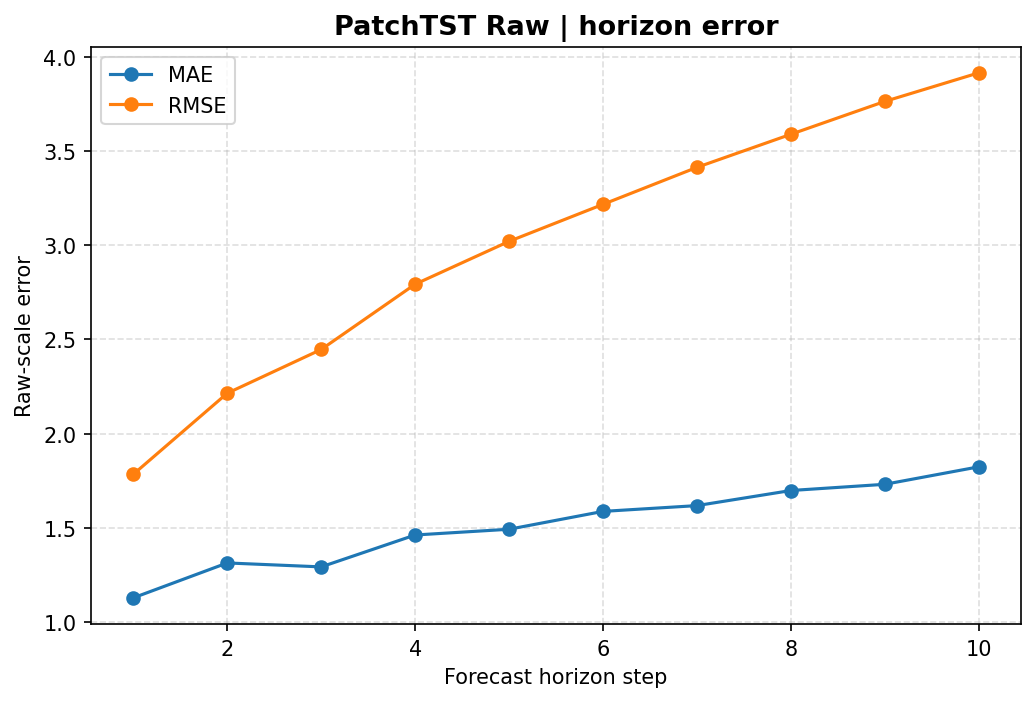
\includegraphics[width=0.82\textwidth]{results/autoregressive_patchtst_raw_horizon_error.png}
  \caption{Horizon-wise forecast error for the PatchTST raw autoregressive model on the external holdout split.}
  \label{fig:autoregressive-patchtst-horizon-error}
\end{figure}

\subsection{Switch Performance}
\label{sec:results-autoregressive-switch-performance}

\Cref{tab:autoregressive-switch-results} reports the switch metrics obtained
after applying the trajectory-to-switch rule and the shared post-processing.
The ranking differs from the pure forecast-error ranking. PatchTST raw has the
best F1 and IoU, even though it is not the best model in RMSE.

\begin{table}[htbp]
  \centering
  \caption{Autoregressive switch performance against Perfect Switch on the external holdout split.}
  \label{tab:autoregressive-switch-results}
  \small
  \setlength{\tabcolsep}{5pt}
  \renewcommand{\arraystretch}{1.15}
  \begin{tabular}{
    @{}
    >{\raggedright\arraybackslash}p{0.38\textwidth}
    rrrr
    @{}
  }
    \toprule
    Method & Precision \(\uparrow\) & Recall \(\uparrow\) & F1 \(\uparrow\) & IoU \(\uparrow\) \\
    \midrule
    PatchTST raw & 0.779 & 0.839 & 0.808 & 0.678 \\
    XGBoost raw & 0.692 & 0.943 & 0.798 & 0.664 \\
    GRU Seq2Seq raw & 0.619 & 0.980 & 0.759 & 0.611 \\
    Chronos zero-shot raw & 0.567 & 0.961 & 0.713 & 0.554 \\
    XGBoost context-standard & 0.512 & 0.991 & 0.675 & 0.510 \\
    GRU S2V raw & 0.509 & 0.993 & 0.674 & 0.508 \\
    PatchTST context-standard & 0.496 & 0.991 & 0.661 & 0.493 \\
    GRU S2V context-standard & 0.496 & 0.987 & 0.660 & 0.493 \\
    GRU Seq2Seq context-standard & 0.497 & 0.985 & 0.660 & 0.493 \\
    \bottomrule
  \end{tabular}
\end{table}

Point-wise precision, recall, F1, and IoU do not fully describe the operational
behavior of a switch policy. Two models can have similar F1 while producing
different active durations or a different number of switch activations. For this
reason, \cref{fig:autoregressive-switch-duration-events} reports the total
post-processed switch duration and the number of contiguous switch islands on
the external holdout split. The Perfect Switch contains 459 active samples,
corresponding to \SI{229.5}{min}, grouped into 18 switch islands. PatchTST raw
is the closest autoregressive model in this diagnostic view, with 494 active
samples and 20 islands. Several other models reach high recall by keeping the
switch active for much longer or by producing many more islands, which explains
their lower precision.

\begin{figure}[H]
  \centering
  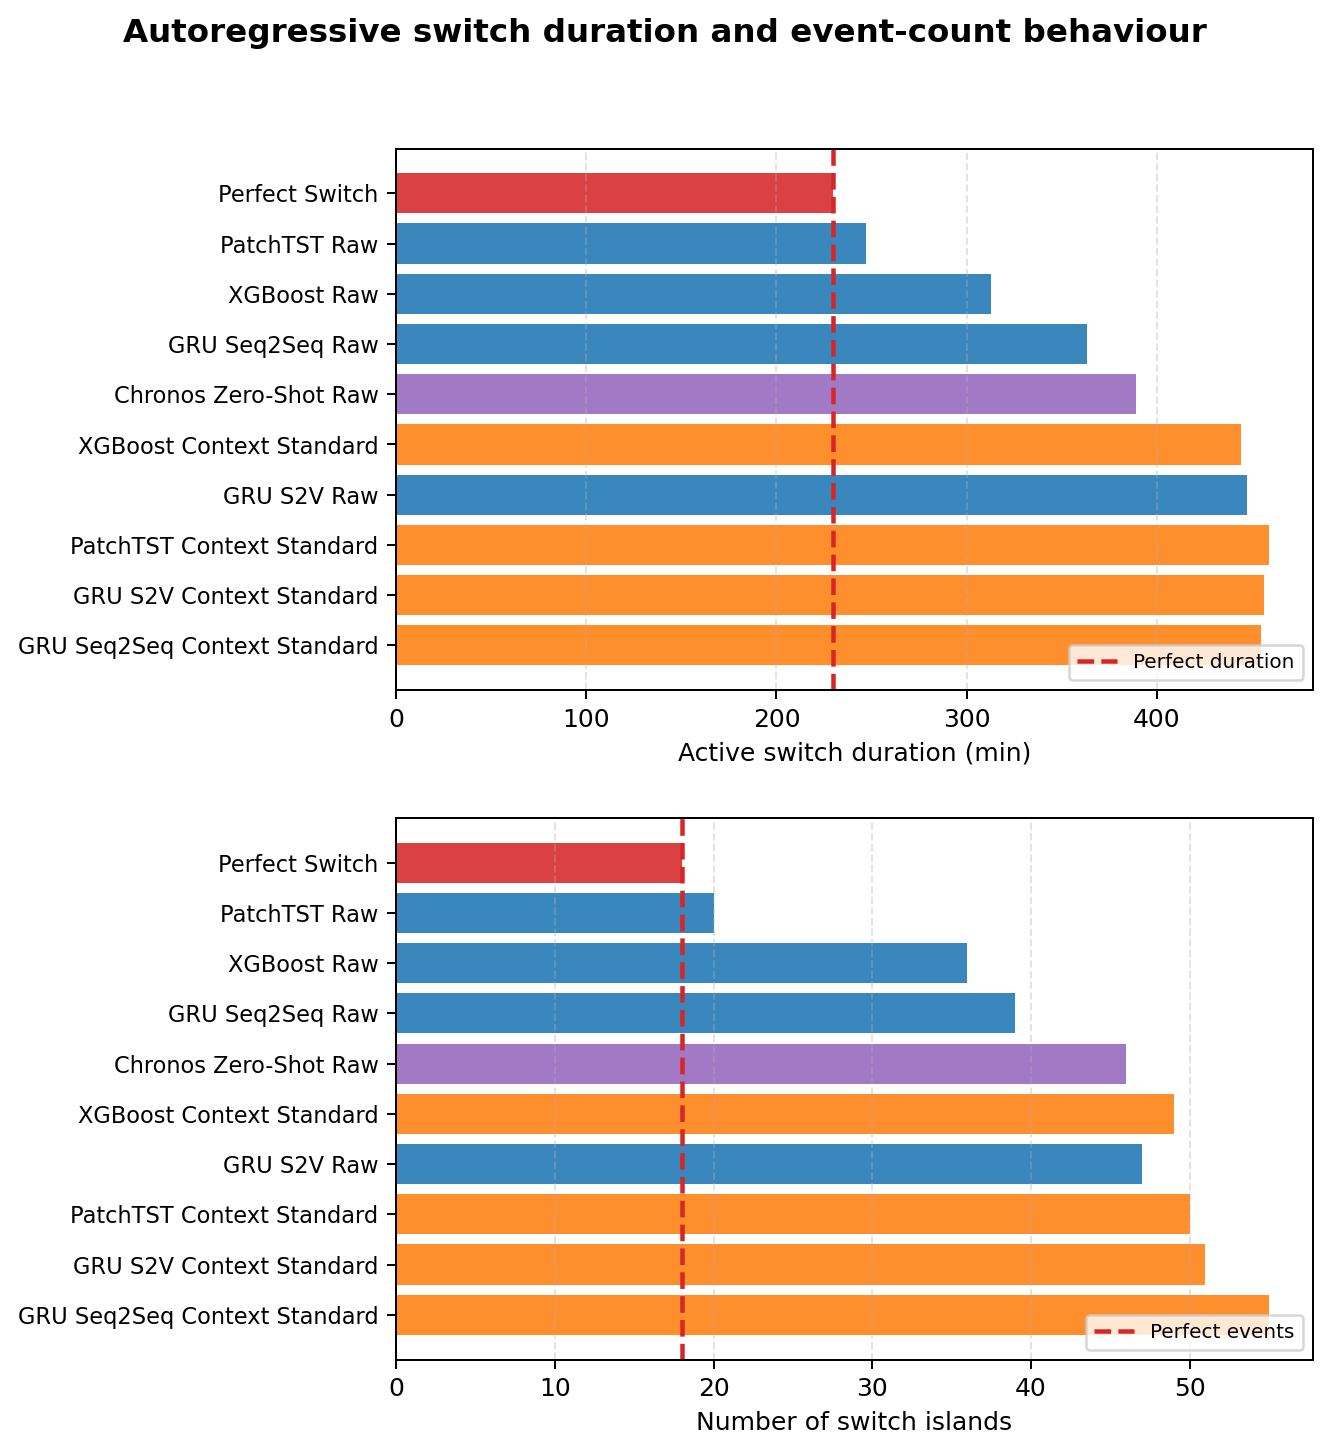
\includegraphics[width=0.8\textwidth]{results/autoregressive_switch_duration_events.png}
  \caption{Autoregressive switch duration and event-count behavior on the external holdout split. Duration counts post-processed positive switch samples, converted to minutes using the \SI{30}{s} sampling time. The dashed red line marks the Perfect Switch value.}
  \label{fig:autoregressive-switch-duration-events}
\end{figure}

The common pattern is high recall and lower precision. In operational terms,
most Perfect Switch points are detected, but several models keep the switch
active for longer than the reference. The raw PatchTST model is the most
balanced among the autoregressive models: it sacrifices some recall relative to
the GRU models, but reduces false positives enough to obtain the highest F1 and
IoU. XGBoost raw is close behind and is notable because it reaches competitive
switch performance without an explicit neural sequence architecture.

The confusion counts clarify this trade-off. PatchTST raw detects 385 of 459
Perfect Switch samples and misses 74, while adding 109 false-positive switch
samples over 7708 evaluated timestamps. This corresponds to a balanced accuracy
of 0.912 and a false-positive rate of 0.015. Its advantage is therefore not
that it detects every switch sample, but that it preserves most operational
intervals while keeping unnecessary switch time limited. The
context-standardized variants have the opposite tendency: they often increase
recall, but they lose precision because local standardization removes part of
the absolute-level information needed near the \SI{10.0}{dB} threshold.

\subsection{Interpretation and Event-Level Examples}
\label{sec:results-autoregressive-examples}


\begin{figure}[H]
  \centering
  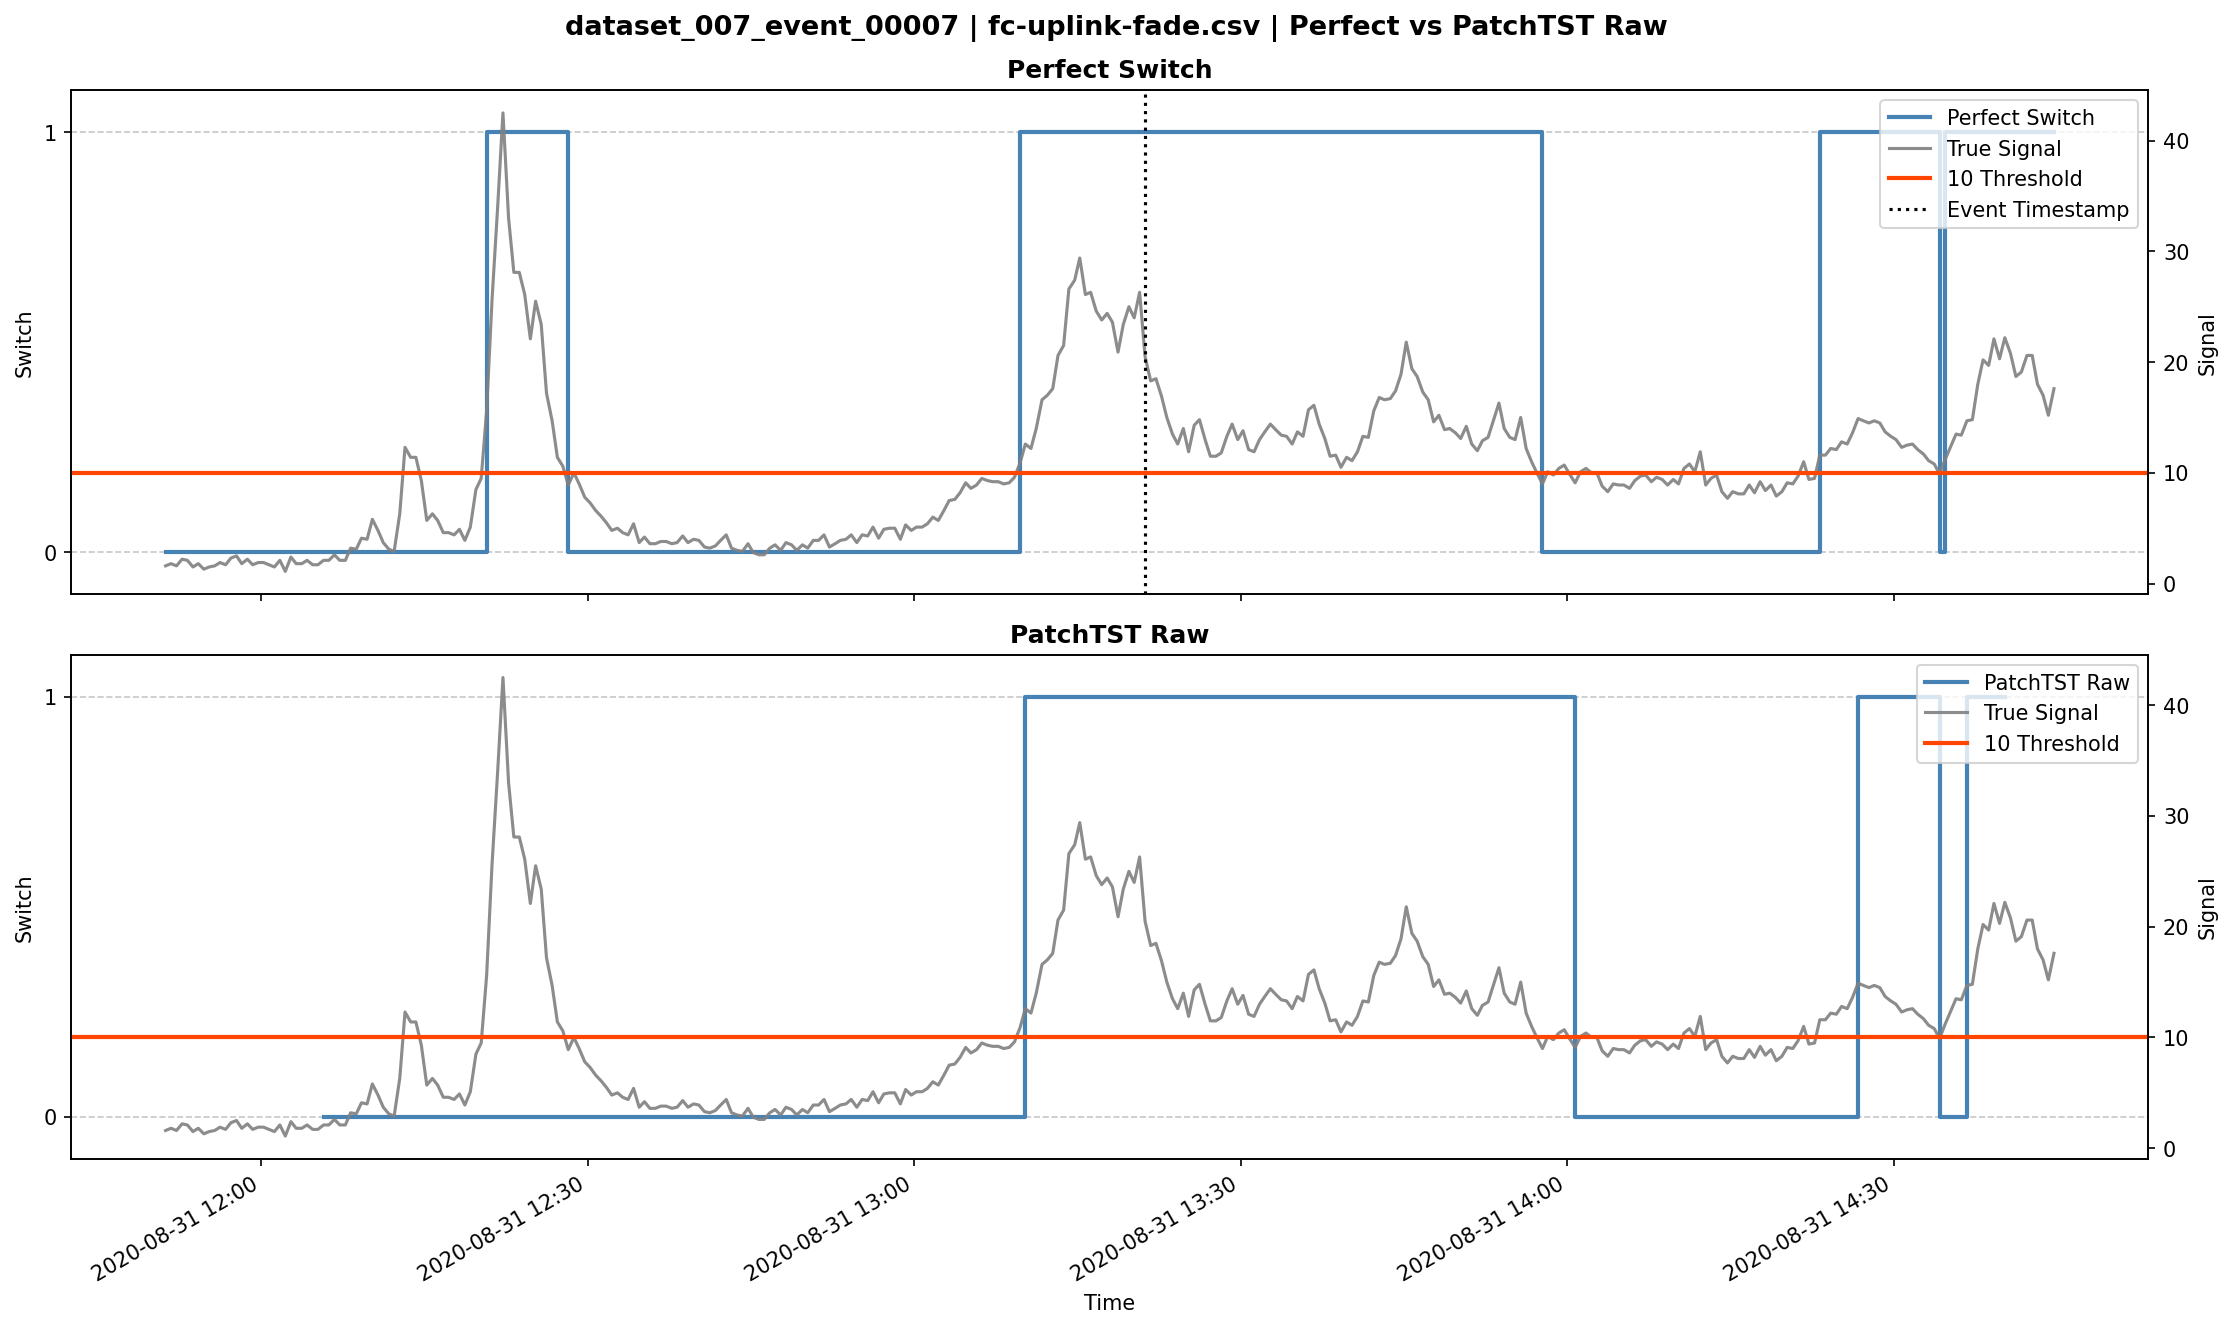
\includegraphics[width=\textwidth]{results/autoregressive_patchtst_raw_event_00007_switch_comparison.png}
  \caption{Example autoregressive switch comparison for PatchTST raw on a multi-interval external-holdout event. The model-derived switch is compared with the Perfect Switch reference after applying the common post-processing rule.}
  \label{fig:autoregressive-patchtst-switch-example}
\end{figure}

\Cref{fig:autoregressive-patchtst-switch-example} shows event
\texttt{dataset\_007\_event\_00007}, which is more informative than a single
isolated fade because the Perfect Switch turns on and off several times. The
upper panel contains the Perfect Switch reference, while the lower panel
contains the PatchTST raw decision. The model captures the long central switch
interval and the late reactivation, but misses the first short
activation. This illustrates why switch metrics are not determined only by
point forecast error: a model can tolerate moderate forecast deviations if it
still preserves the operational threshold crossing structure.


\Cref{fig:autoregressive-switch-mosaic} compares all autoregressive switch
decisions on event 00003 of dataset 007, a different, single-interval example
from \cref{fig:autoregressive-patchtst-switch-example}.
The upper panel shows the raw signal and the
\SI{10.0}{dB} threshold, while each lower row shows the final post-processed
switch sequence for one method. This compact view makes clear that most
autoregressive models identify the main fade, but they slightly differ in onset timing,
release timing, and the amount of extra switch activity around the event.

\begin{figure}[H]
  \centering
  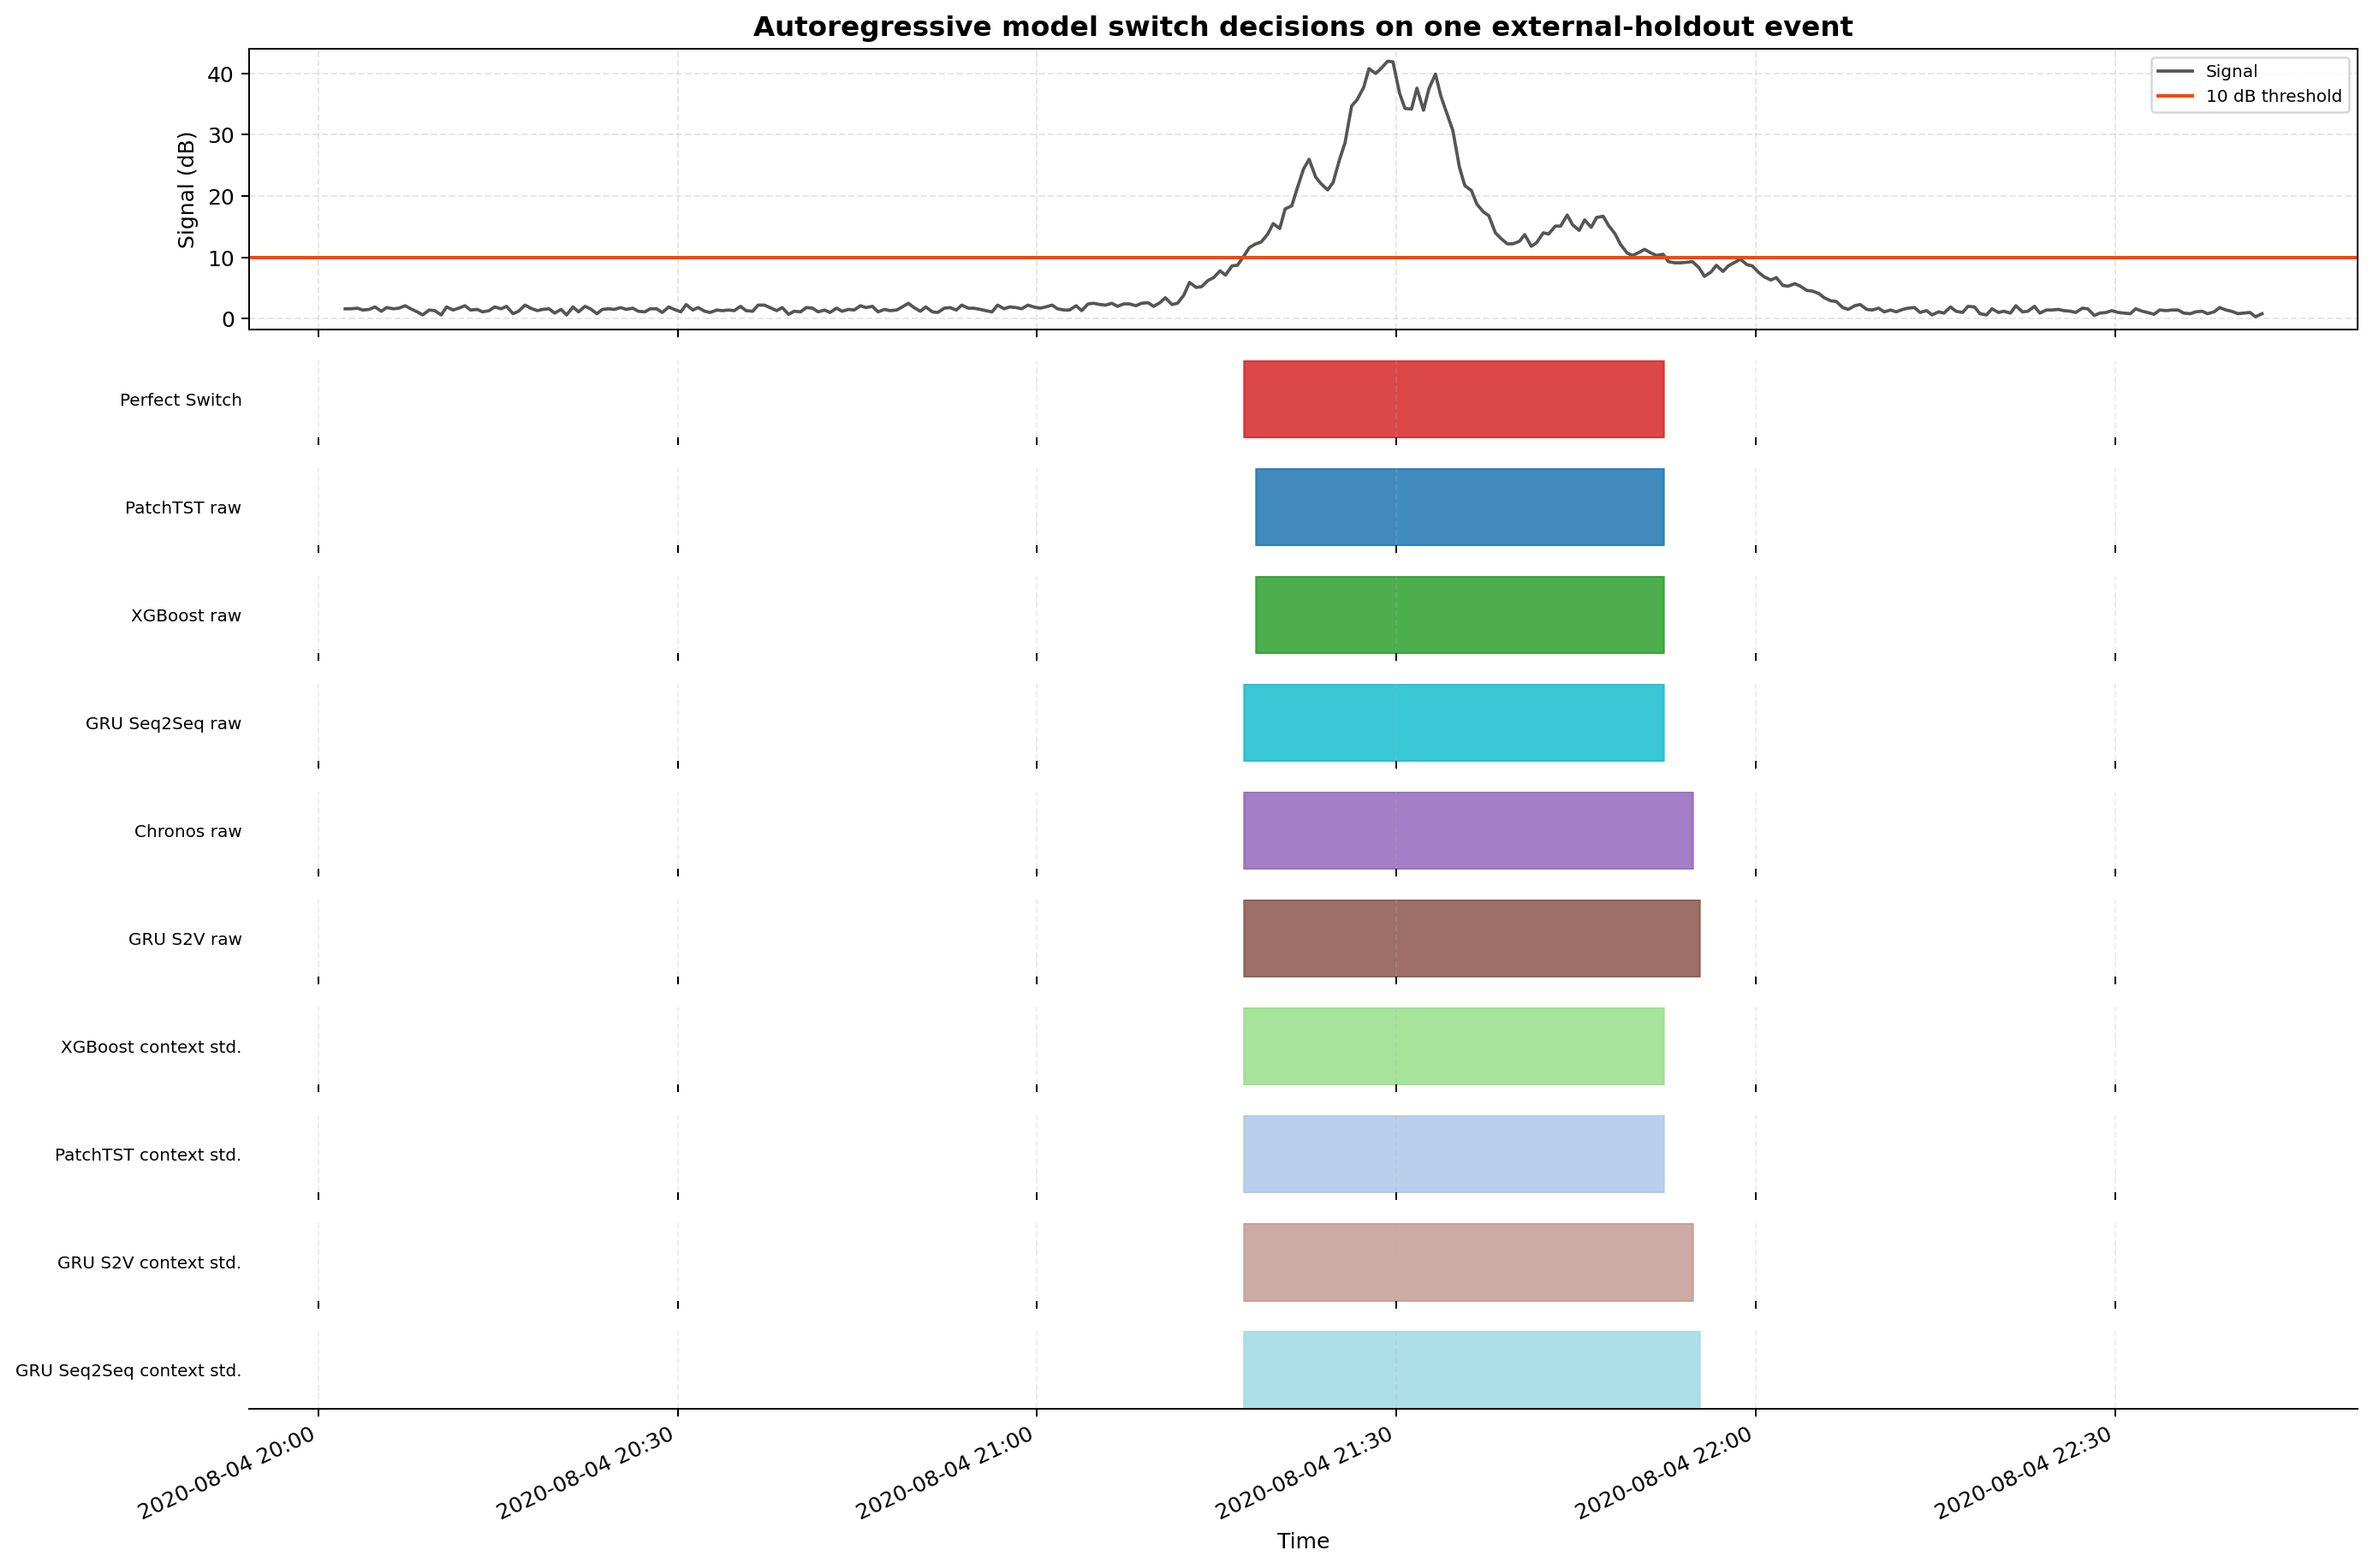
\includegraphics[width=0.95\textwidth]{results/autoregressive_event00003_switch_mosaic.png}
  \caption{Mosaic of post-processed switch decisions for all autoregressive methods on one external-holdout event. Each row reports the final switch used for evaluation, not the raw thresholded model output.}
  \label{fig:autoregressive-switch-mosaic}
\end{figure}

\section{Current-Level Persistence}
\label{sec:results-current-level-persistence}

The current-level persistence task predicts how long the signal will remain
above \(S_i-\delta\), with \(\delta=\SI{0.5}{dB}\). This is a scalar duration
regression problem, not a future-trajectory forecast. A switch is requested only
when the current signal is at least \(\SI{10.0}{dB}\) and the predicted
remaining persistence is at least \SI{300}{s}; the same switch post-processing
used for the other tasks is then applied.

\subsection{Duration Prediction Accuracy}
\label{sec:results-current-level-duration}

\Cref{tab:current-level-duration-results} reports the validation and test
duration-regression metrics. Errors are expressed in seconds because the
operational threshold is \SI{300}{s}. The table also reports the median
absolute error, which is important because the target distribution is highly
right-skewed: a small number of very long persistence intervals can dominate
MAE and especially RMSE.

\begin{table}[htbp]
  \centering
  \caption{Current-level persistence duration-regression results on the external holdout split. All error metrics are expressed in seconds.}
  \label{tab:current-level-duration-results}
  \small
  \setlength{\tabcolsep}{4pt}
  \renewcommand{\arraystretch}{1.15}
  \begin{tabular}{
    @{}
    >{\raggedright\arraybackslash}p{0.34\textwidth}
    rrrr
    @{}
  }
    \toprule
    Method
      & \shortstack{Val. MAE\\\((\mathrm{s})\,\downarrow\)}
      & \shortstack{Test MAE\\\((\mathrm{s})\,\downarrow\)}
      & \shortstack{Test RMSE\\\((\mathrm{s})\,\downarrow\)}
      & \shortstack{Test median AE\\\((\mathrm{s})\,\downarrow\)} \\
    \midrule
    XGBoost scalar context & 1220.9 & 586.9 & 2584.6 & 27.2 \\
    Shapelet convolution scalar context & 4613.2 & 1835.6 & 6491.0 & 141.5 \\
    Shapelet MLP scalar context & 5116.5 & 2063.8 & 7629.7 & 160.6 \\
    Shapelet Transformer scalar context & 5278.9 & 2056.6 & 7685.3 & 169.4 \\
    \bottomrule
  \end{tabular}
\end{table}

XGBoost is clearly the strongest model for this formulation. Its test median
absolute error is only \SI{27.2}{s}, which means that typical short-horizon
decisions are often accurate. However, its test MAE is \SI{586.9}{s} and its
RMSE is \SI{2584.6}{s}, showing that large errors still occur on long
persistence intervals. The learnable-shapelet models are substantially worse:
their test MAE is around \SI{30}{min} to \SI{34}{min}, and their RMSE exceeds
\SI{108}{min}. These errors are too large for the scalar duration prediction to
be considered reliable by itself.

\Cref{fig:current-level-duration-errors} summarizes the same behavior in
minutes. The median errors are much smaller than the mean errors, confirming
that the hard cases are concentrated in the long tail of the duration
distribution rather than uniformly distributed over all windows.

\begin{figure}[H]
  \centering
  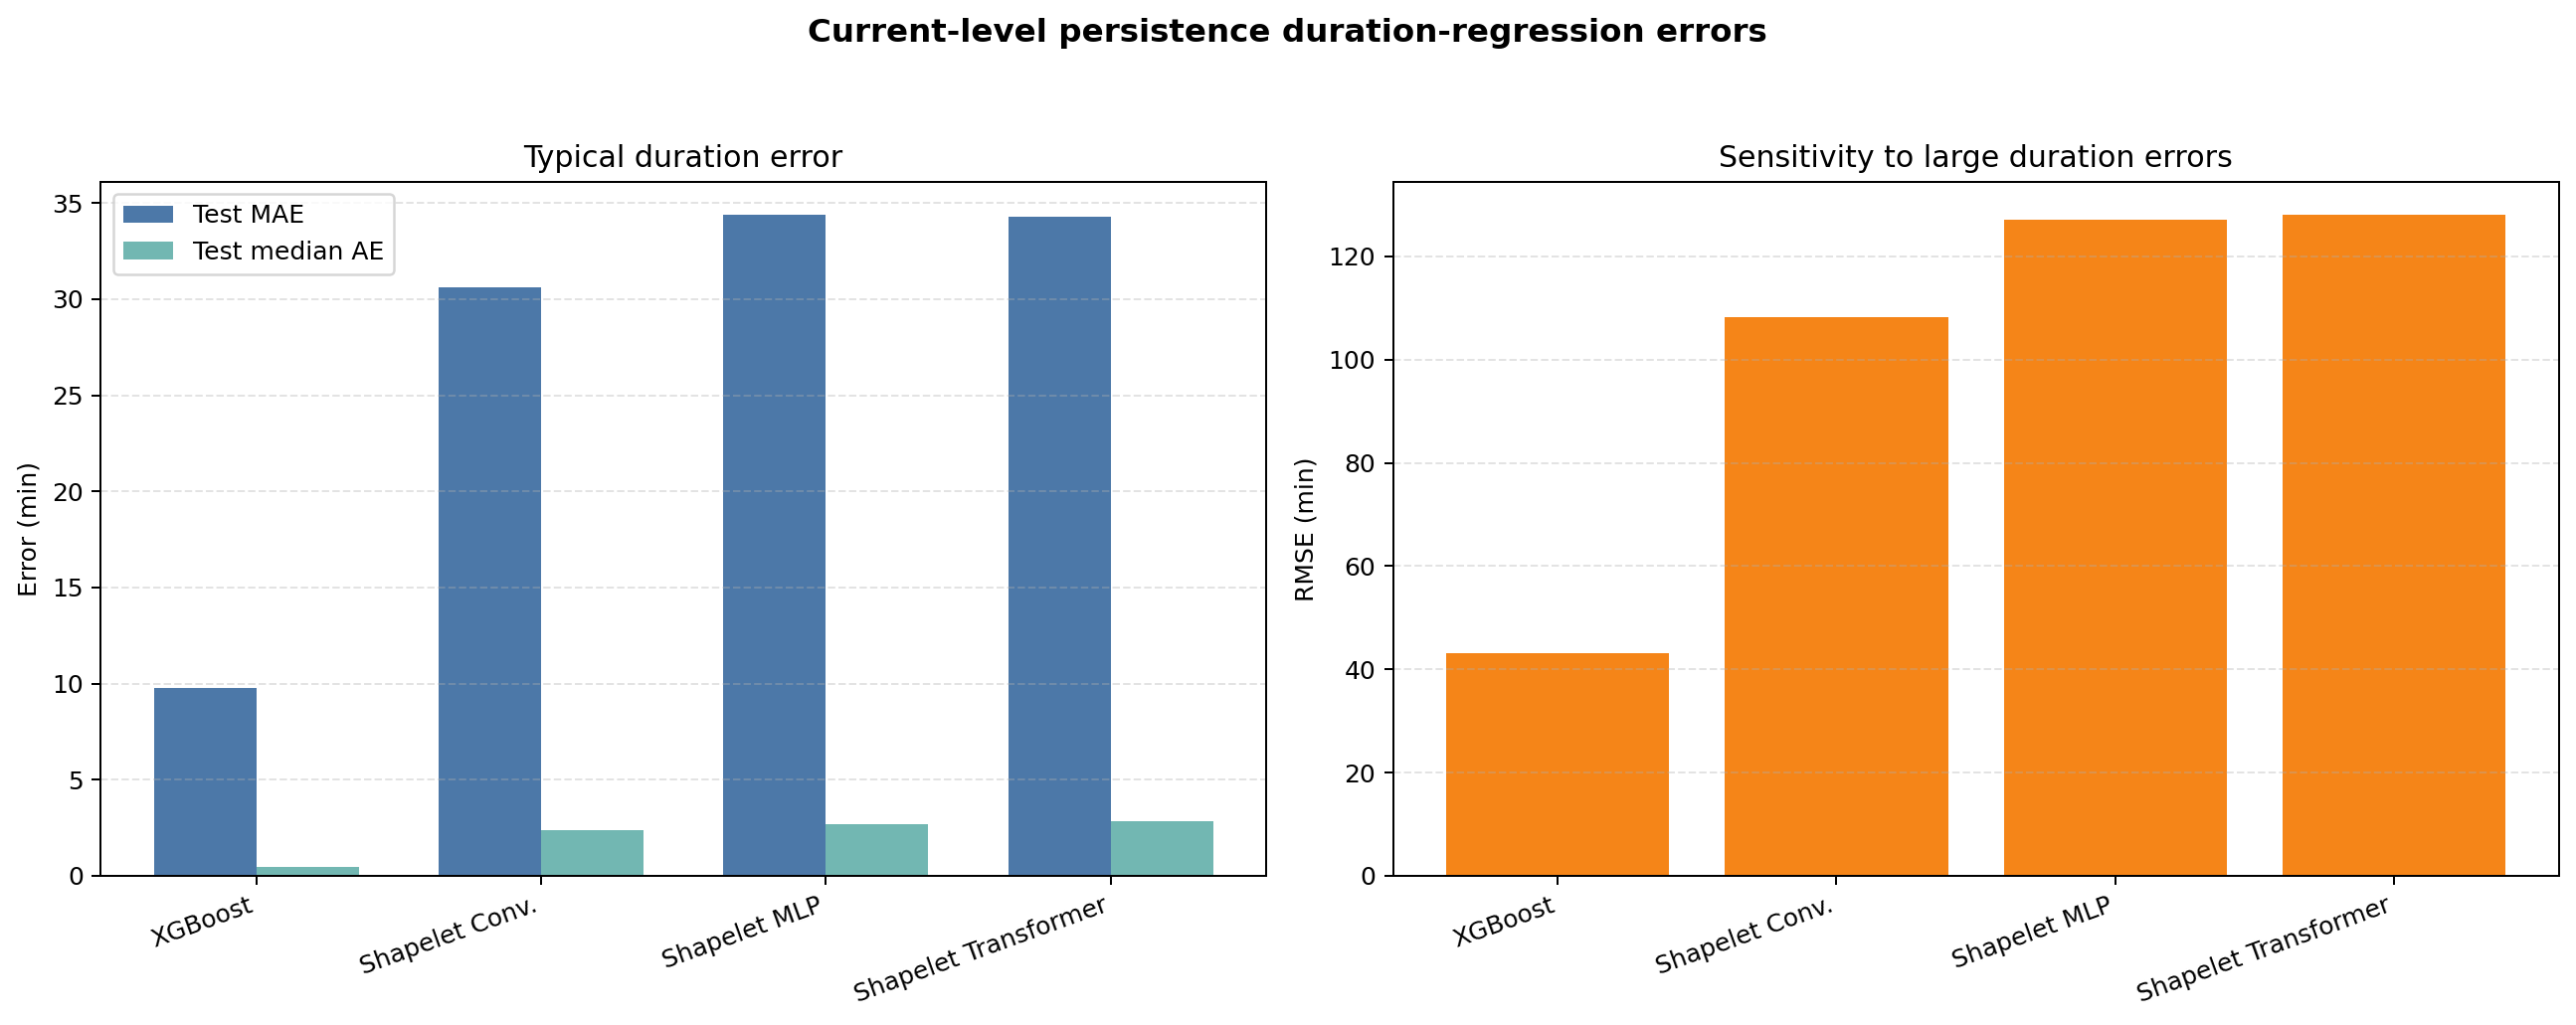
\includegraphics[width=\textwidth]{results/current_level_duration_errors.png}
  \caption{Current-level persistence duration-regression errors on the external holdout split. MAE and median absolute error describe typical behavior, while RMSE highlights sensitivity to long-duration mistakes.}
  \label{fig:current-level-duration-errors}
\end{figure}

\Cref{fig:current-level-xgboost-duration-scatter} shows the predicted and true
durations for the best current-level model. The dense region near the origin is
well aligned, but the dispersion increases for longer intervals. This explains
why the median absolute error is low while MAE and RMSE remain large.

\begin{figure}[H]
  \centering
  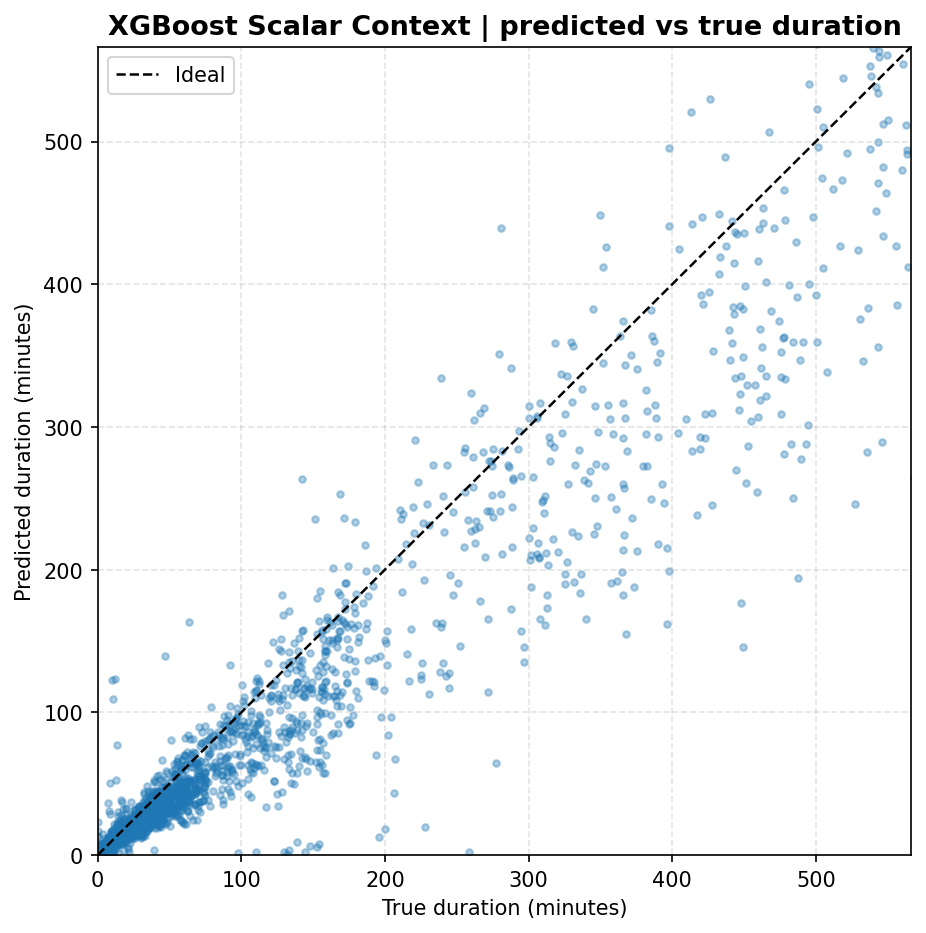
\includegraphics[width=0.60\textwidth]{results/current_level_xgboost_duration_predicted_vs_true.png}
  \caption{Predicted versus true current-level persistence duration for the XGBoost scalar-context model on the external holdout split.}
  \label{fig:current-level-xgboost-duration-scatter}
\end{figure}

\subsection{Switch Performance}
\label{sec:results-current-level-switch}

\Cref{tab:current-level-switch-results} reports the resulting switch metrics.
Despite the imperfect duration regression, XGBoost gives a useful switch
policy: it reaches an F1 score of \(0.902\) and produces no false-positive
switch samples on the external holdout split. The three learnable-shapelet
models instead produce an all-zero final switch sequence, so they obtain zero
recall and zero F1. This is not caused by missing predictions. The signal gate
is active at 672 test timestamps, but the maximum persistence predicted at
those timestamps is only \SI{148.8}{s} for the shapelet MLP, \SI{204.6}{s} for
the shapelet Transformer, and \SI{167.3}{s} for the shapelet convolution model.
All remain below the \SI{300}{s} duration threshold. The same models do predict
durations above \SI{300}{s} at other timestamps, but only when the current
signal is below \SI{10.0}{dB}. Consequently, the two conditions required by the
decision rule are never true simultaneously. This is an operationally
important negative result: the models fit the regression target to some extent,
but they are not usable switch controllers under the configured rule.

\begin{table}[htbp]
  \centering
  \caption{Current-level persistence switch performance against Perfect Switch on the external holdout split.}
  \label{tab:current-level-switch-results}
  \small
  \setlength{\tabcolsep}{5pt}
  \renewcommand{\arraystretch}{1.15}
  \begin{tabular}{
    @{}
    >{\raggedright\arraybackslash}p{0.38\textwidth}
    rrrrr
    @{}
  }
    \toprule
    Method & Precision \(\uparrow\) & Recall \(\uparrow\) & F1 \(\uparrow\) & IoU \(\uparrow\) & Active min. \\
    \midrule
    XGBoost scalar context & 1.000 & 0.822 & 0.902 & 0.822 & 189.5 \\
    Shapelet MLP scalar context & 0.000 & 0.000 & 0.000 & 0.000 & 0.0 \\
    Shapelet Transformer scalar context & 0.000 & 0.000 & 0.000 & 0.000 & 0.0 \\
    Shapelet convolution scalar context & 0.000 & 0.000 & 0.000 & 0.000 & 0.0 \\
    \bottomrule
  \end{tabular}
\end{table}

\Cref{fig:current-level-switch-duration-events} makes this contrast explicit.
The Perfect Switch has 461 active samples, corresponding to \SI{230.5}{min},
and 17 switch islands. XGBoost produces 379 active samples and 11 islands. It
therefore under-covers part of the Perfect Switch, but its conservative
behavior avoids the excessive switch activity observed in several
autoregressive variants. The shapelet models produce no active switch interval
under the configured decision rule.

This result should be read together with the decision rule. A current-level
model is allowed to request a switch only when the current signal is already at
or above the \SI{10.0}{dB} threshold and the predicted persistence exceeds
\SI{300}{s}. The XGBoost model therefore behaves as a conservative switch
policy: it produces 379 true-positive switch samples, no false-positive samples,
and 82 false negatives. The resulting precision of 1.000 is operationally
attractive because every requested switch is aligned with the reference, but
the recall loss indicates that some useful backup-link intervals would be
missed. This is a different failure mode from autoregressive forecasting, where
the main issue is excess active duration rather than missed coverage.

\begin{figure}[H]
  \centering
  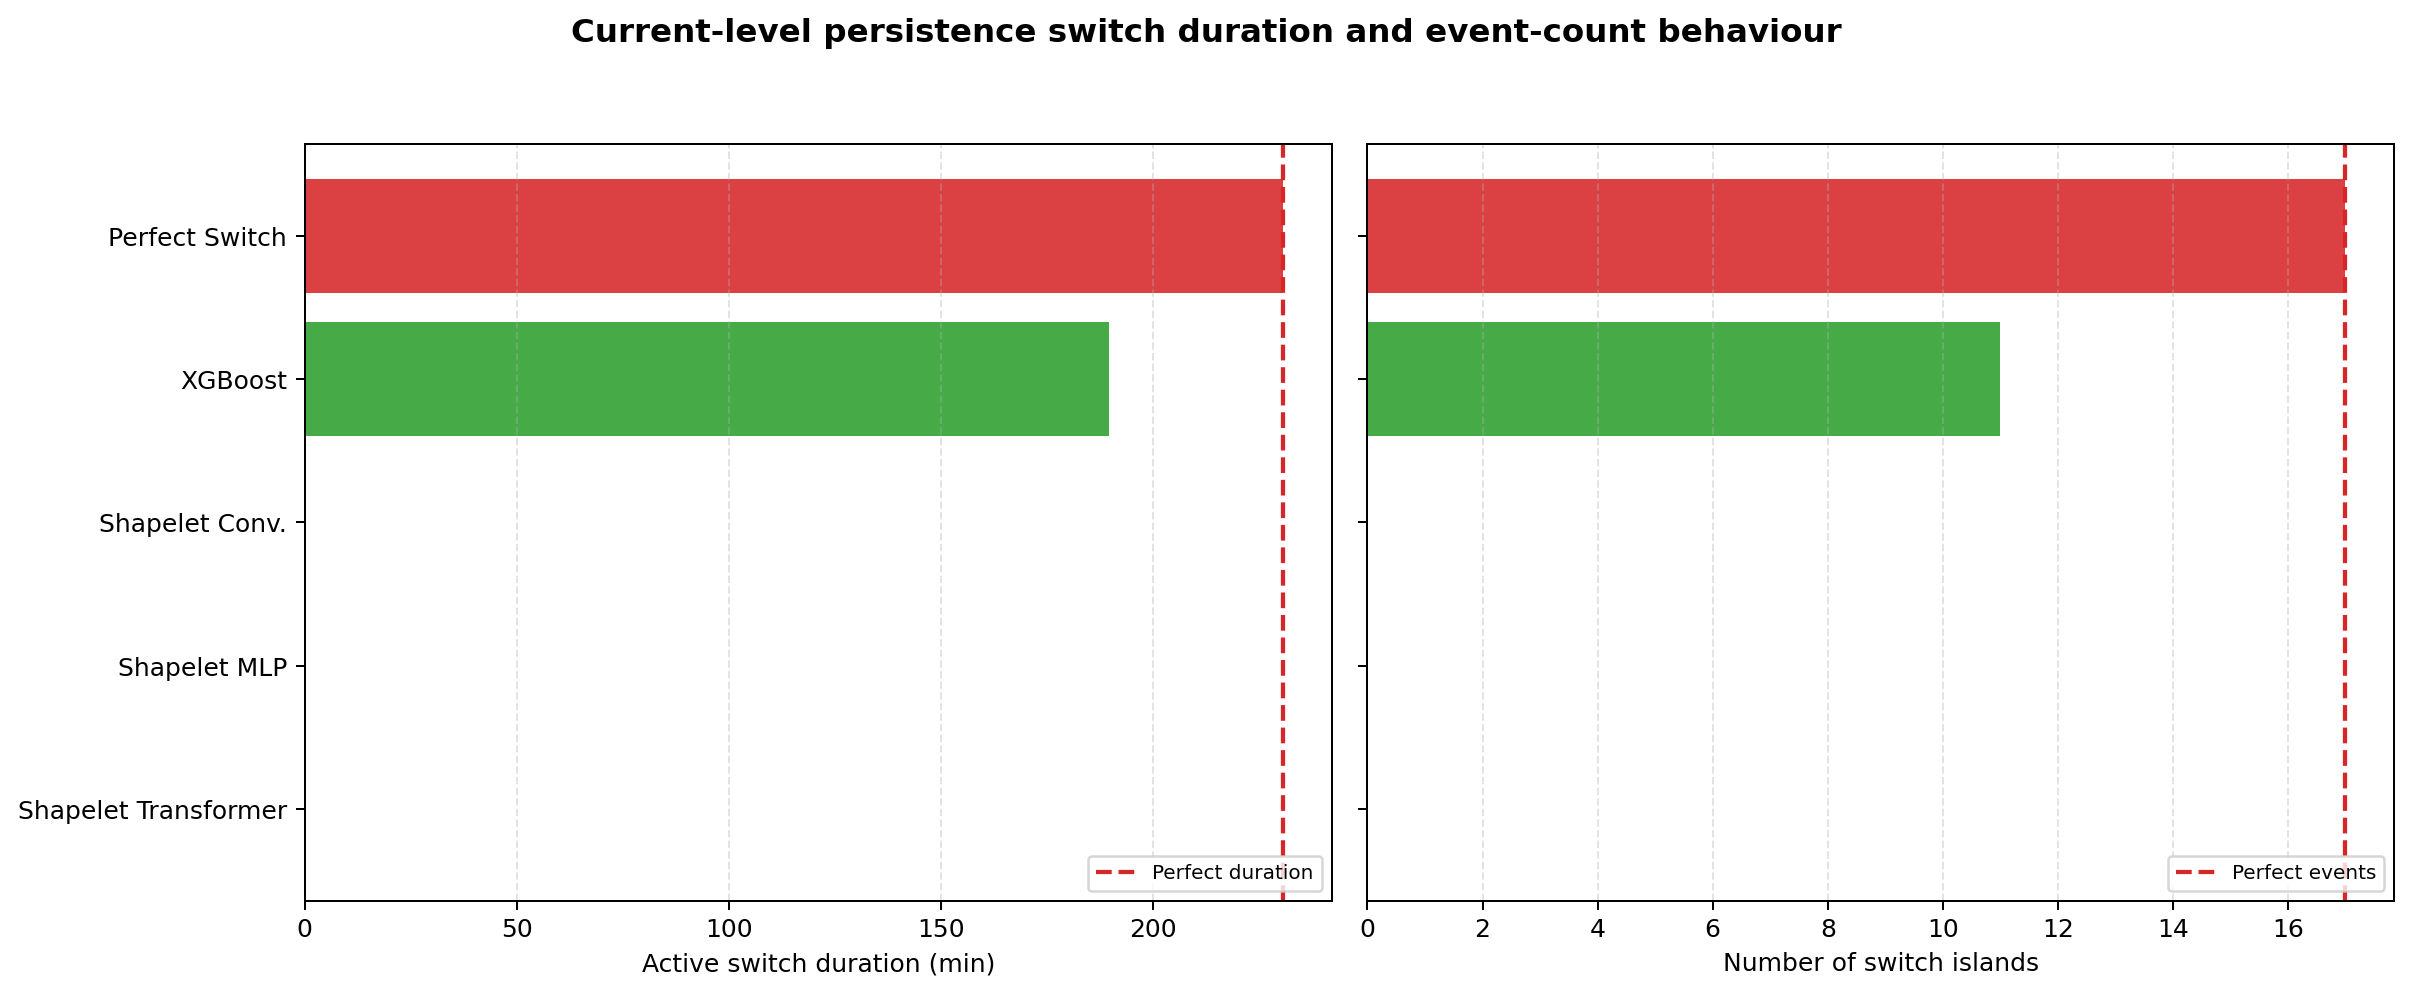
\includegraphics[width=\textwidth]{results/current_level_switch_duration_events.png}
  \caption{Current-level persistence switch duration and event-count behavior on the external holdout split. Duration counts post-processed positive switch samples, converted to minutes using the \SI{30}{s} sampling time.}
  \label{fig:current-level-switch-duration-events}
\end{figure}

\subsection{Interpretation and Event-Level Examples}
\label{sec:results-current-level-examples}


\begin{figure}[H]
  \centering
  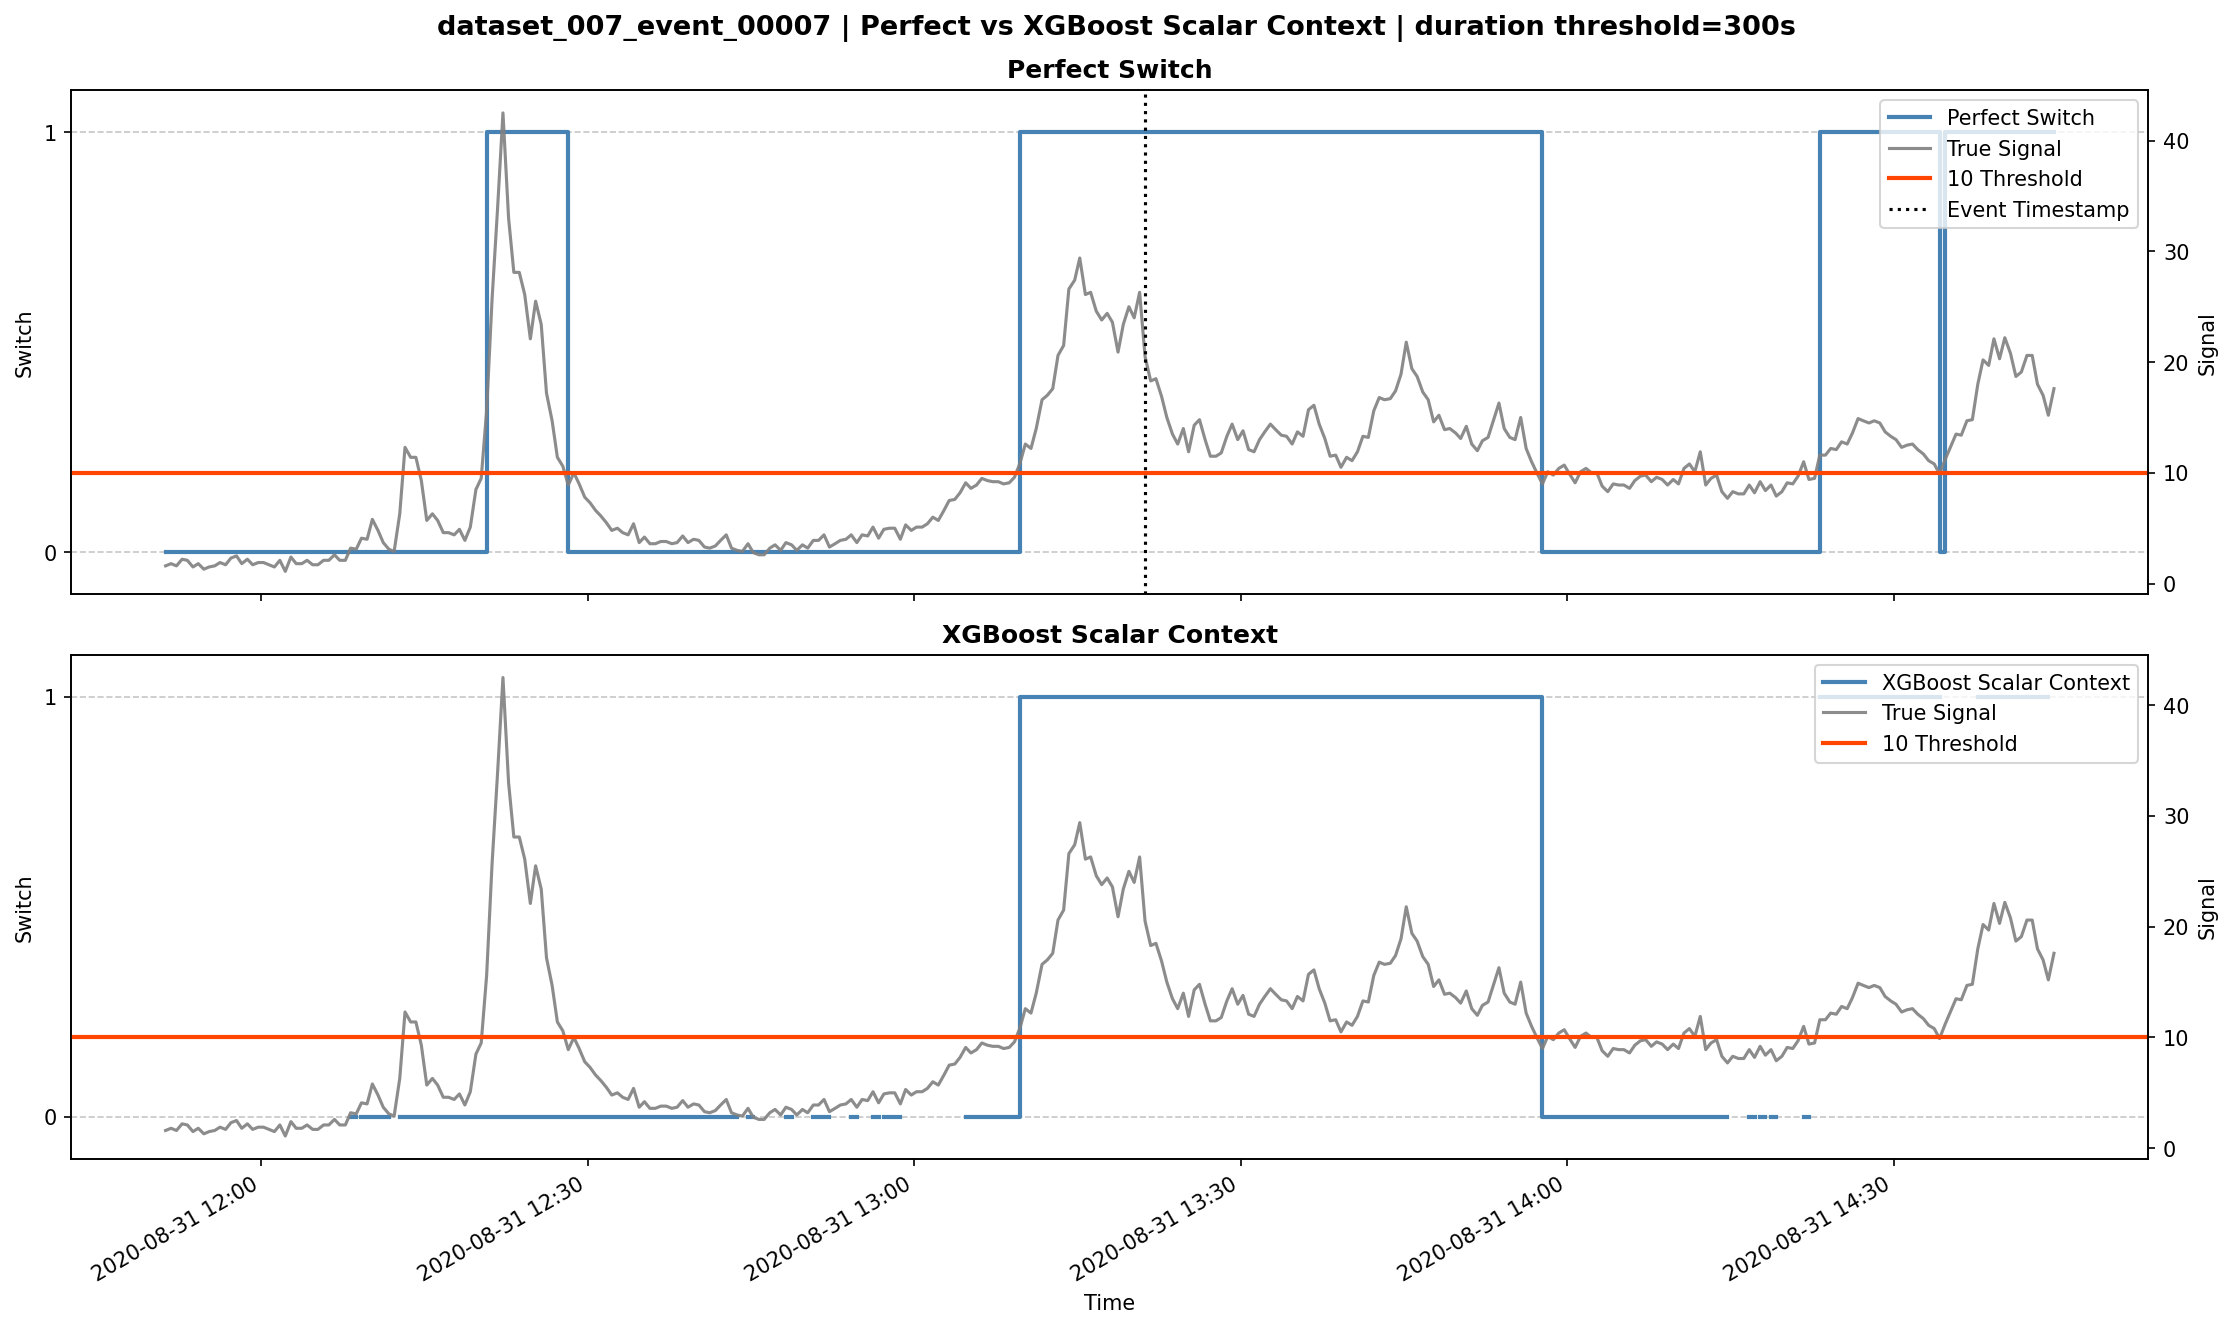
\includegraphics[width=0.9\textwidth]{results/current_level_xgboost_event_00007_switch_comparison.png}
  \caption{Example current-level persistence switch comparison for XGBoost scalar context on the selected multi-interval external-holdout event. The model-derived switch is compared with the Perfect Switch reference after applying the common post-processing rule.}
  \label{fig:current-level-xgboost-switch-example}
\end{figure}



\Cref{fig:current-level-xgboost-switch-example} shows the current-level
XGBoost model on the task-native decision grid for the same source event
identifier used in \cref{fig:autoregressive-patchtst-switch-example}. Because each task has its own
valid decision timestamps, the plotted Perfect Switch can differ slightly
between task-native figures. The model decision follows the long central
interval well and avoids the short early activation. This is consistent with
the global behavior of the task: the model is conservative and does not create
false-positive switch samples, but it can ignore short or marginal intervals
that the Perfect Switch keeps. The example also clarifies the role of the
formulation: the model does not forecast the whole future trajectory; it only
estimates whether the current level is likely to persist long enough to justify
the switch.


\section{Long-Fade Detection}
\label{sec:results-long-fade-detection}

The long-fade detection task is a binary classification problem defined inside
grouped fade events. At each eligible timestamp, the model estimates whether
the grouped event will last at least \SI{300}{s}. The native output is therefore
a class probability, not a duration or a future signal trajectory. For switch
evaluation, a switch is requested when the predicted long-fade probability is at
least \(0.5\), followed by the same shared switch post-processing used in the
other tasks.

\subsection{Classification Metrics}
\label{sec:results-long-fade-classification}

\Cref{tab:long-fade-classification-results} reports the native classification
metrics. All three models reach very high validation and test AUPRC. This
indicates that the long-fade label is easy to separate once the sample is known
to belong to a grouped fade event. The result must therefore be interpreted with
care: the task is useful as an event-level persistence classifier, but its
native metrics are less demanding than the final switch decision because the
dataset excludes most non-event background timestamps.

\begin{table}[htbp]
  \centering
  \caption{Long-fade detection classification results on the external holdout split.}
  \label{tab:long-fade-classification-results}
  \small
  \setlength{\tabcolsep}{4pt}
  \renewcommand{\arraystretch}{1.15}
  \begin{tabular}{
    @{}
    >{\raggedright\arraybackslash}p{0.36\textwidth}
    rrrr
    @{}
  }
    \toprule
    Method
      & \shortstack{Val. AUPRC\\\(\uparrow\)}
      & \shortstack{Test AUPRC\\\(\uparrow\)}
      & \shortstack{Test AUROC\\\(\uparrow\)}
      & \shortstack{Test F1@0.5\\\(\uparrow\)} \\
    \midrule
    TCN classifier & 1.000 & 1.000 & 1.000 & 0.999 \\
    XGBoost lag + scalar & 1.000 & 1.000 & 1.000 & 1.000 \\
    Shapelet convolution classifier & 1.000 & 1.000 & 0.999 & 0.997 \\
    \bottomrule
  \end{tabular}
\end{table}

The TCN and XGBoost classifiers are almost indistinguishable in native
classification space. The shapelet convolution model is slightly weaker on the
test split, but it remains close to the other two models. The stronger
differences appear only after the probabilities are converted into switch
sequences and compared with the Perfect Switch reference.

\subsection{Switch Performance}
\label{sec:results-long-fade-switch}

\Cref{tab:long-fade-switch-results} reports the switch metrics obtained after
thresholding the predicted probabilities and applying the shared
post-processing. All models recover nearly all Perfect Switch samples, but this
comes at the cost of many false-positive switch samples. The TCN has the best
F1 and IoU, closely followed by XGBoost.

\begin{table}[htbp]
  \centering
  \caption{Long-fade detection switch performance against Perfect Switch on the external holdout split.}
  \label{tab:long-fade-switch-results}
  \small
  \setlength{\tabcolsep}{5pt}
  \renewcommand{\arraystretch}{1.15}
  \begin{tabular}{
    @{}
    >{\raggedright\arraybackslash}p{0.38\textwidth}
    rrrrr
    @{}
  }
    \toprule
    Method & Precision \(\uparrow\) & Recall \(\uparrow\) & F1 \(\uparrow\) & IoU \(\uparrow\) & Active min. \\
    \midrule
    TCN classifier & 0.540 & 1.000 & 0.702 & 0.540 & 445.0 \\
    XGBoost lag + scalar & 0.540 & 1.000 & 0.701 & 0.540 & 445.5 \\
    Shapelet convolution classifier & 0.521 & 0.998 & 0.685 & 0.521 & 460.5 \\
    \bottomrule
  \end{tabular}
\end{table}

\Cref{fig:long-fade-switch-duration-events} shows why the switch scores are
lower than the native classification scores. The Perfect Switch contains 481
active samples, corresponding to \SI{240.5}{min}, and 19 switch islands on the
long-fade evaluation grid. The model-derived switches contain almost twice as
many active samples and more than twice as many islands. This means that the
models correctly identify long fades, but they keep the switch active over a
broader portion of the grouped-event windows than the Perfect Switch requires.

For the TCN classifier, the confusion matrix contains no false negatives: all
481 Perfect Switch samples are detected. The cost is 409 false-positive
samples, a false-positive rate of 0.196, and 890 active switch samples in
total. This explains why the recall is 1.000 but the precision is only 0.540.
The result is not a modeling failure in the native classification task; it is
a consequence of converting a grouped-event label into an instantaneous switch
policy. Once a grouped fade is classified as long, the model tends to remain
positive over a wide portion of that grouped event, including regions where the
Perfect Switch has already turned off.

\begin{figure}[H]
  \centering
  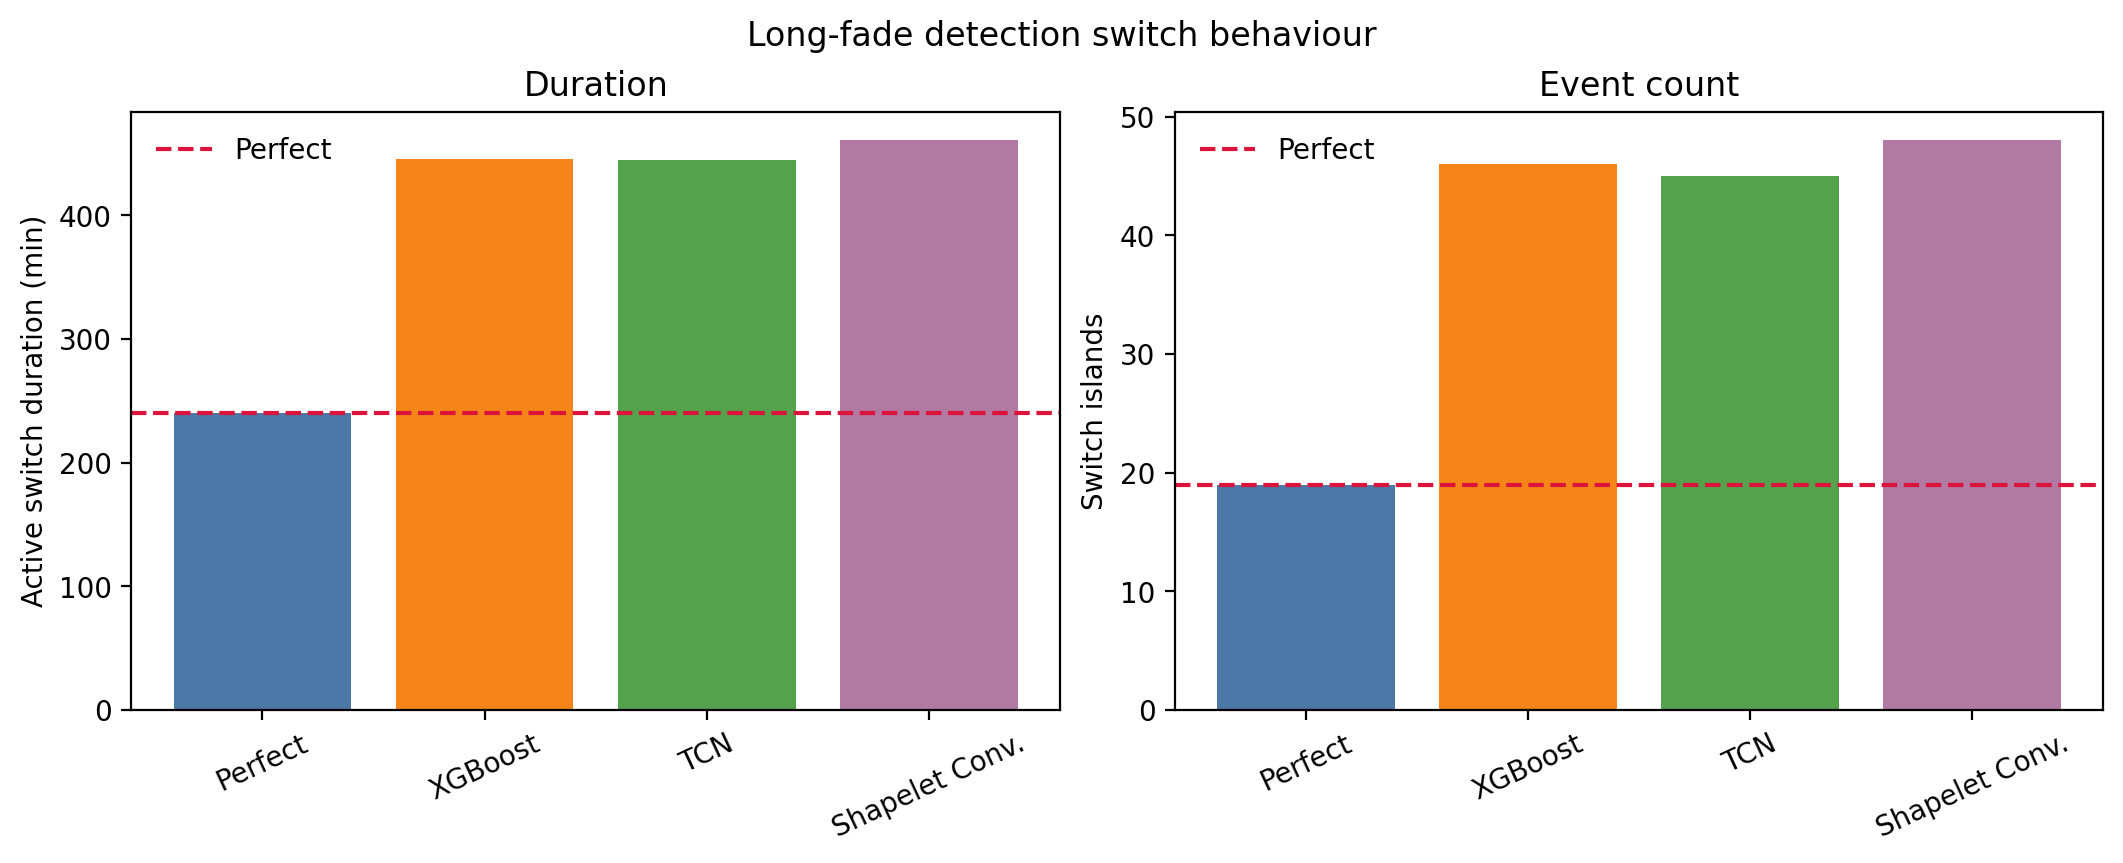
\includegraphics[width=\textwidth]{results/long_fade_switch_duration_events.png}
  \caption{Long-fade detection switch duration and event-count behavior on the external holdout split. Duration counts post-processed positive switch samples, converted to minutes using the \SI{30}{s} sampling time. The dashed red line marks the Perfect Switch value.}
  \label{fig:long-fade-switch-duration-events}
\end{figure}

\subsection{Interpretation and Event-Level Examples}
\label{sec:results-long-fade-examples}

\begin{figure}[H]
  \centering
  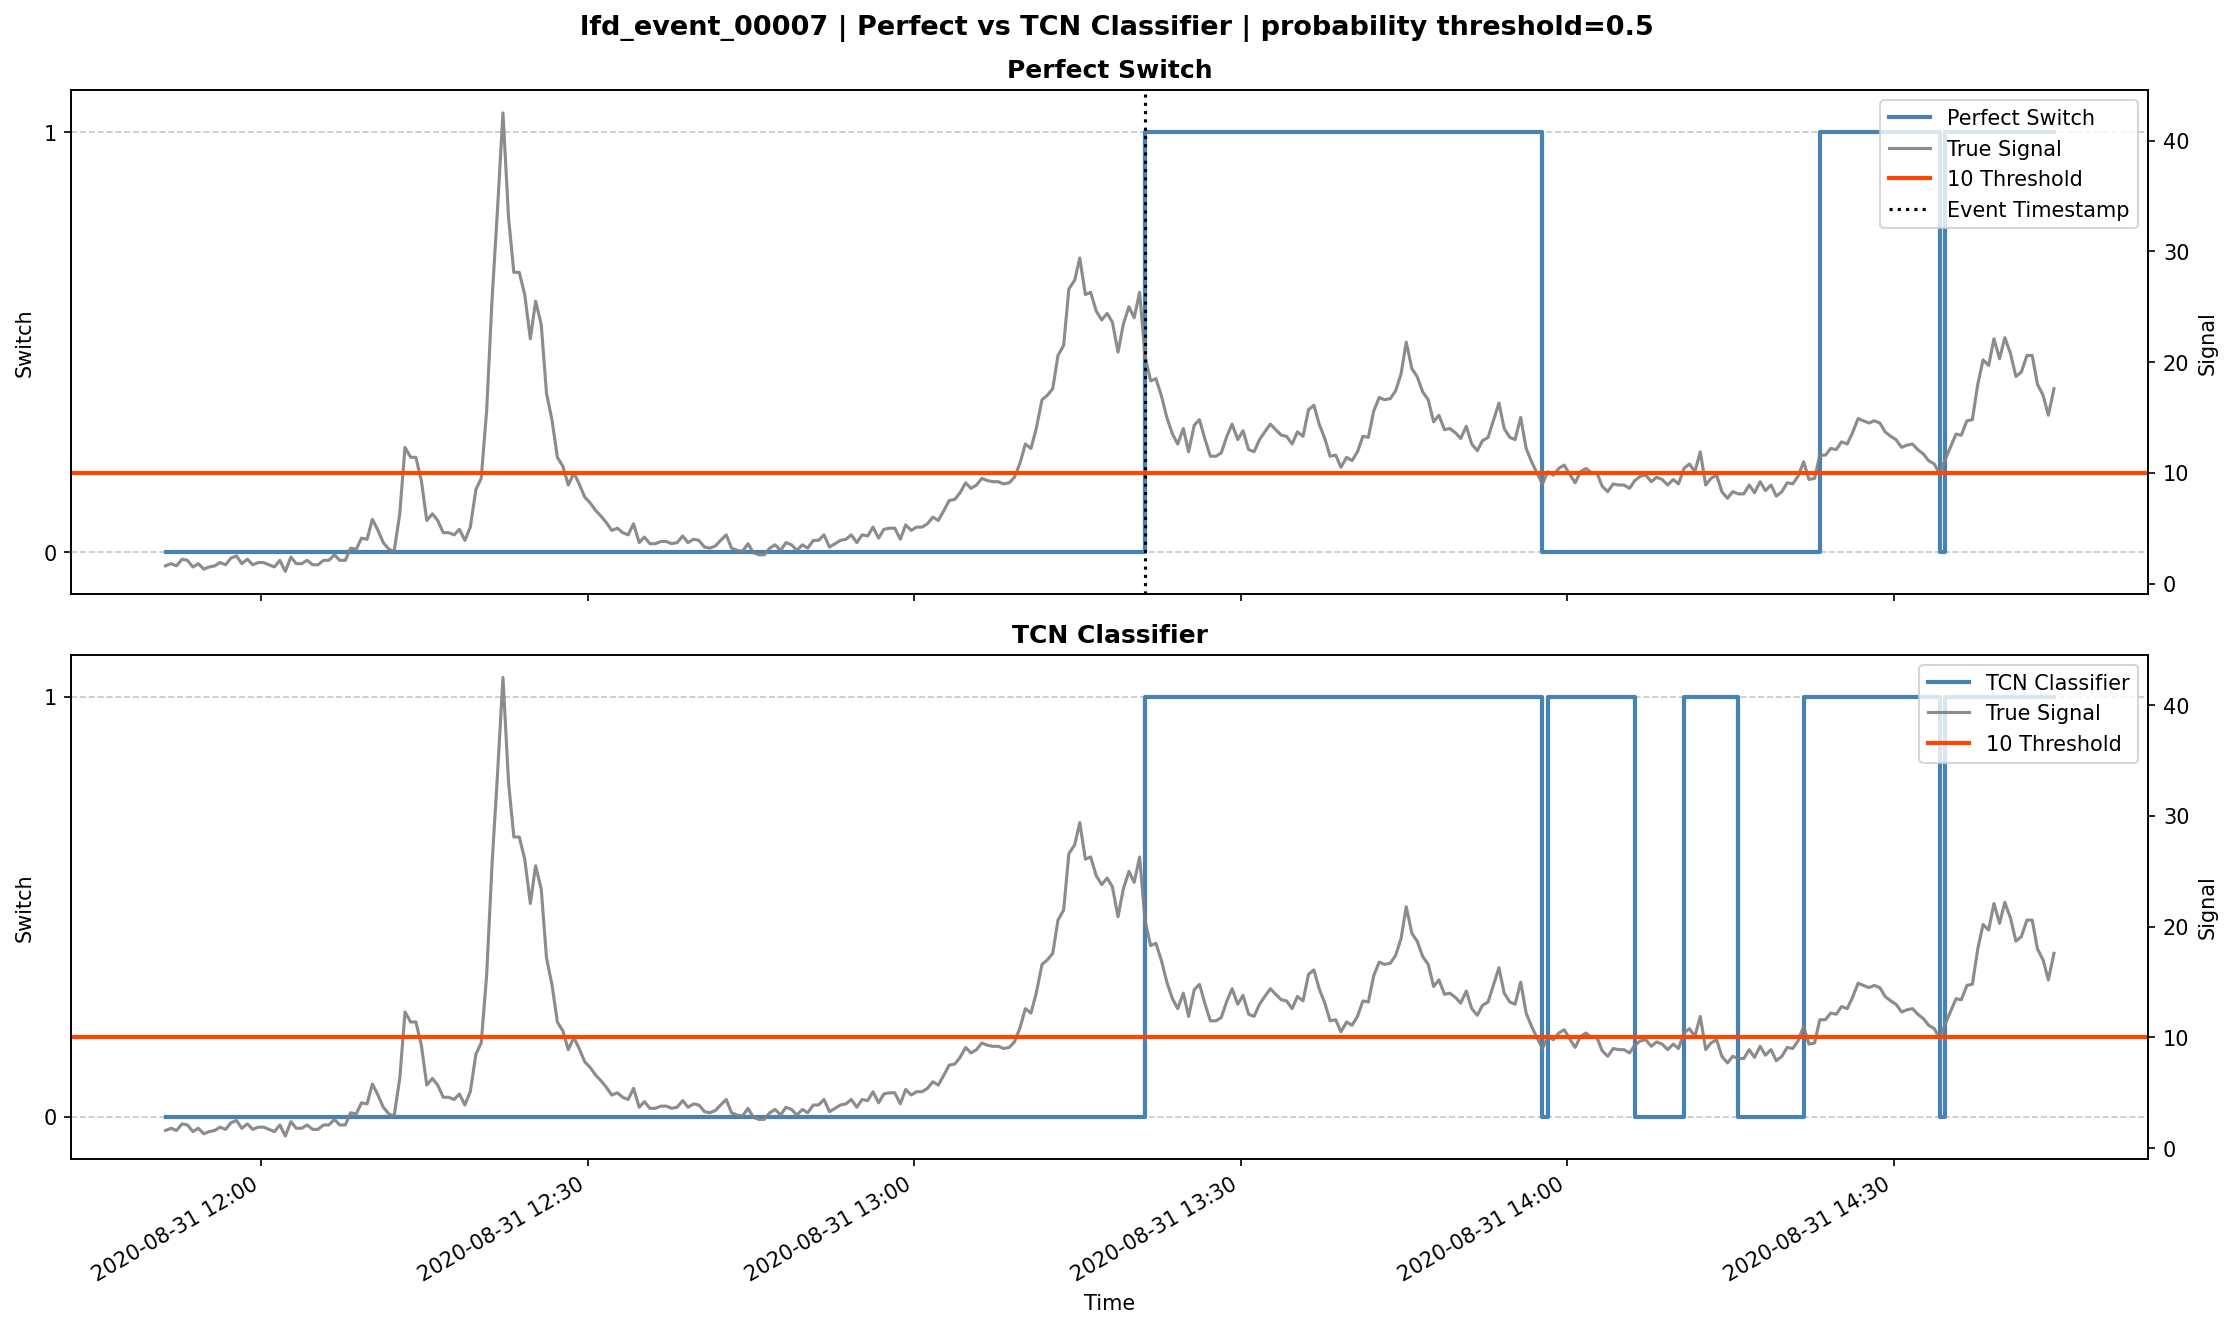
\includegraphics[width=\textwidth]{results/long_fade_tcn_event_00007_switch_comparison.png}
  \caption{Example long-fade detection switch comparison for the TCN classifier on the selected multi-interval external-holdout event. The model-derived switch is compared with the Perfect Switch reference after applying the common post-processing rule.}
  \label{fig:long-fade-tcn-switch-example}
\end{figure}

\Cref{fig:long-fade-tcn-switch-example} shows a task-native long-fade event for
the TCN classifier. The event number is local to the long-fade dataset and
should not be interpreted as the same global event number used in the previous
task-native figures. The model recognizes the grouped event as a long fade and
keeps the switch active over most of the grouped region. This makes the
formulation robust to temporary oscillations around the threshold, but it is
less precise than the Perfect Switch when the operational reference contains
several separate on/off intervals. The example therefore illustrates the main
trade-off of long-fade detection: it is a reliable high-recall detector of
problematic events, but it is too coarse to be the most selective switch
controller. The wider signal window provides context; switch values outside
the native event segment are displayed as zero and are not evaluated.



Overall, long-fade detection is highly effective at recognizing whether a
grouped fade is long, but it is less precise as a direct switch policy. It
therefore behaves as a high-recall formulation: useful when missed long fades
are especially costly, but less attractive when unnecessary switch duration is
penalized heavily.

\section{Survival Persistence}
\label{sec:results-survival-persistence}

The survival persistence task estimates the distribution of the remaining fade
duration rather than a single deterministic target. The evaluated models output
survival probabilities \(S(u \mid X_i)\), where \(u\) is a future duration
horizon. The operational switch rule uses the \SI{300}{s} horizon: a switch is
requested when \(S(\SI{300}{s}\mid X_i)\geq 0.65\) and the current signal is at
least \(\SI{10.0}{dB}\). The probability threshold \(0.65\) is retained as an
exploratory operating point from the switch-analysis stage; it should not be
interpreted as a fully validation-calibrated threshold.

\subsection{Survival Metrics}
\label{sec:results-survival-metrics}

\Cref{tab:survival-results} reports the native survival metrics on the external
holdout split. The two models are evaluated on the same censored survival
dataset. The XGBoost-AFT model uses continuous lower and upper survival bounds,
whereas the discrete-time TCN predicts hazards on a fixed duration grid. For
this reason, likelihood values are model-specific diagnostics; the comparison
below focuses on Harrell's C-index, integrated Brier score, and horizon-specific
Brier and calibration errors.

\begin{table}[htbp]
  \centering
  \caption{Survival persistence metrics on the external holdout split.}
  \label{tab:survival-results}
  \small
  \setlength{\tabcolsep}{4pt}
  \renewcommand{\arraystretch}{1.15}
  \begin{tabular}{
    @{}
    >{\raggedright\arraybackslash}p{0.34\textwidth}
    rrrr
    @{}
  }
    \toprule
    Method & C-index \(\uparrow\) & IBS \(\downarrow\) & Brier@300s \(\downarrow\) & Calib. error@300s \(\downarrow\) \\
    \midrule
    XGBoost-AFT & 0.672 & 0.117 & 0.218 & 0.123 \\
    Discrete-time TCN & 0.658 & 0.103 & 0.214 & 0.105 \\
    \bottomrule
  \end{tabular}
\end{table}

The two models show different strengths. The C-index point estimate of
XGBoost-AFT exceeds that of the discrete-time TCN by (0.014). To assess the
robustness of this difference while preserving dependence among timestamps of
the same event, a paired event-level bootstrap resampled the 55 external-holdout
events 2,000 times. The resulting 95\% percentile interval for the C-index
difference, XGBoost-AFT minus TCN, was ([-0.021, 0.049]). Because this interval
includes zero, the observed gap does not provide evidence of a statistically
significant ranking advantage and should be interpreted only as a small
numerical difference on this test set. Conversely, the discrete-time TCN has
the lower integrated Brier score and lower \SI{300}{s} calibration error,
indicating better probabilistic accuracy over the evaluated time grid. Neither
result alone determines switch quality, because the operational decision uses
only one point on the survival curve and then applies binary post-processing.

\Cref{fig:survival-tcn-curves} illustrates the TCN output using six test
windows selected near the 5th, 23rd, 41st, 59th, 77th, and 95th percentiles of
the predicted \(S(\SI{300}{s}\mid X_i)\) distribution. This replaces a purely
chronological selection, which produced several almost indistinguishable curves
from adjacent timestamps. The legend reports, for each window, its selection
quantile, predicted survival probability at the operational horizon, predicted
median residual duration, and observed residual duration. The selected
\(S(\SI{300}{s}\mid X_i)\) values range from (0.39) to (0.81), and therefore
show materially different operational predictions around the (0.65) switch
threshold. These curves are deterministic predictions for different windows,
not repeated estimates of a common population curve; consequently, a pairwise
statistical-significance test between them is not defined. Residual overlap
instead indicates that the TCN assigns similar hazard profiles to some inputs,
especially at long horizons where all predicted survival probabilities approach
zero.

\begin{figure}[H]
  \centering
  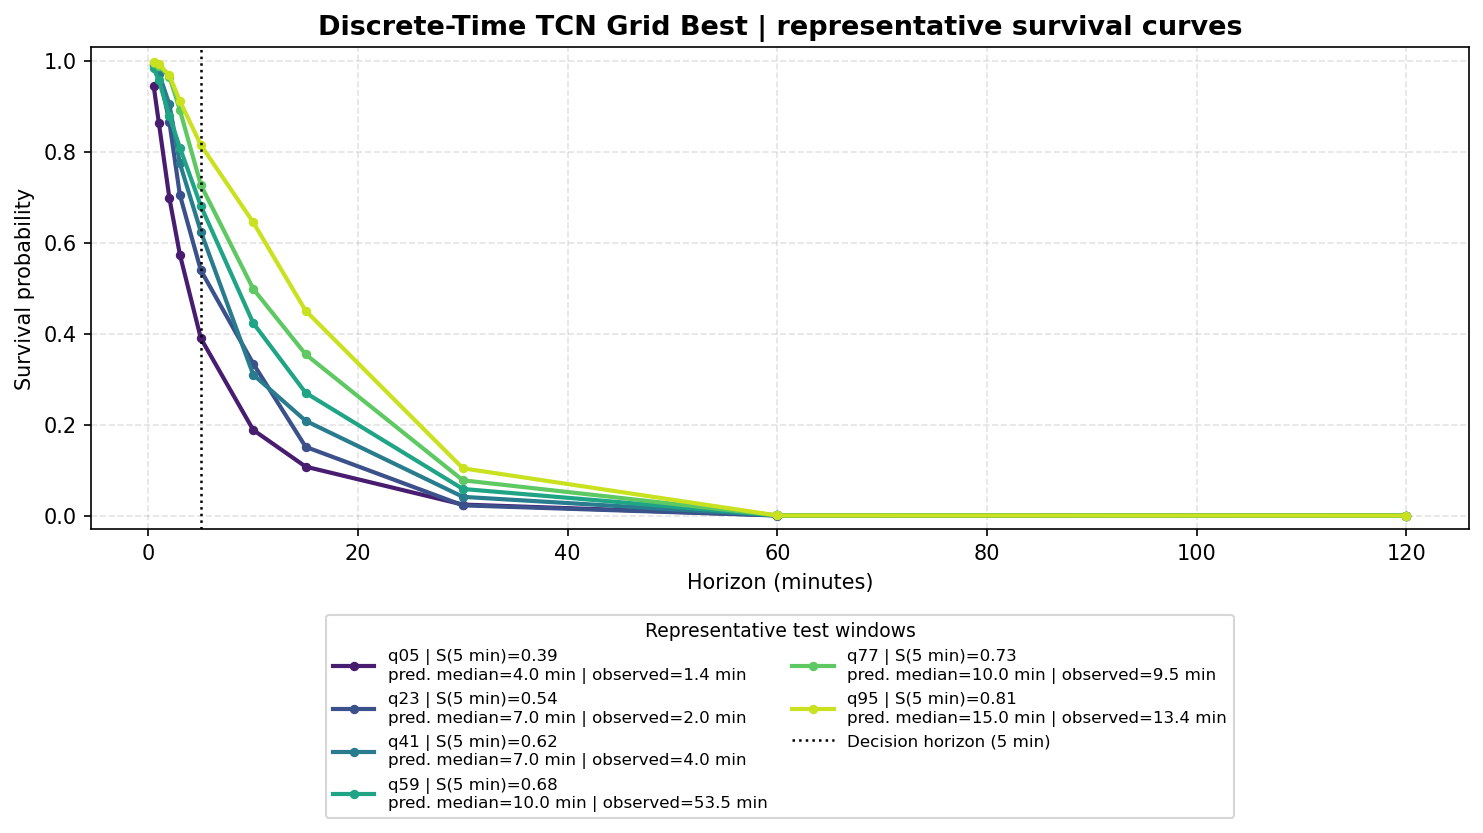
\includegraphics[width=0.98\textwidth]{results/survival_tcn_selected_survival_curves.png}
  \caption{Representative survival curves produced by the discrete-time TCN on the external holdout split. Curves are selected by quantiles of \(S(\SI{300}{s}\mid X_i)\); colors identify the windows described in the legend, and the dotted line marks the \SI{300}{s} operational horizon.}
  \label{fig:survival-tcn-curves}
\end{figure}

\subsection{Switch Performance}
\label{sec:results-survival-switch}

\Cref{tab:survival-switch-results} reports the switch metrics after converting
survival probabilities at \SI{300}{s} into binary decisions. XGBoost-AFT is the
stronger switch model: it reaches higher precision, F1, and IoU than the
discrete-time TCN. The TCN has higher recall, but it does so by keeping the
switch active much more often.

\begin{table}[htbp]
  \centering
  \caption{Survival persistence switch performance against Perfect Switch on the external holdout split.}
  \label{tab:survival-switch-results}
  \small
  \setlength{\tabcolsep}{5pt}
  \renewcommand{\arraystretch}{1.15}
  \begin{tabular}{
    @{}
    >{\raggedright\arraybackslash}p{0.38\textwidth}
    rrrrr
    @{}
  }
    \toprule
    Method & Precision \(\uparrow\) & Recall \(\uparrow\) & F1 \(\uparrow\) & IoU \(\uparrow\) & Active min. \\
    \midrule
    XGBoost-AFT & 0.828 & 0.902 & 0.863 & 0.759 & 299.0 \\
    Discrete-time TCN & 0.657 & 0.971 & 0.784 & 0.644 & 405.5 \\
    \bottomrule
  \end{tabular}
\end{table}

\Cref{fig:survival-switch-duration-events} shows the same difference from an
operational perspective. The Perfect Switch contains 549 active samples,
corresponding to \SI{274.5}{min}, and 22 switch islands on the survival
evaluation grid. XGBoost-AFT is close in duration but produces more switch
islands, while the TCN overextends the active duration and still produces more
islands than the reference.

The XGBoost-AFT switch has 495 true positives, 103 false positives, and 54
false negatives. Compared with current-level persistence, it is less
conservative: it accepts some unnecessary switch time in order to recover more
of the Perfect Switch. Compared with long-fade detection, it is much more
selective: the active duration is close to the reference, and the F1 score rises
to 0.863. This supports the methodological motivation for survival
persistence. Estimating \(P(R_i>u\mid X_i)\) provides a quantity that is already
aligned with the operational question, rather than requiring a trajectory or
event-classification output to be indirectly converted into a switch.

\begin{figure}[H]
  \centering
  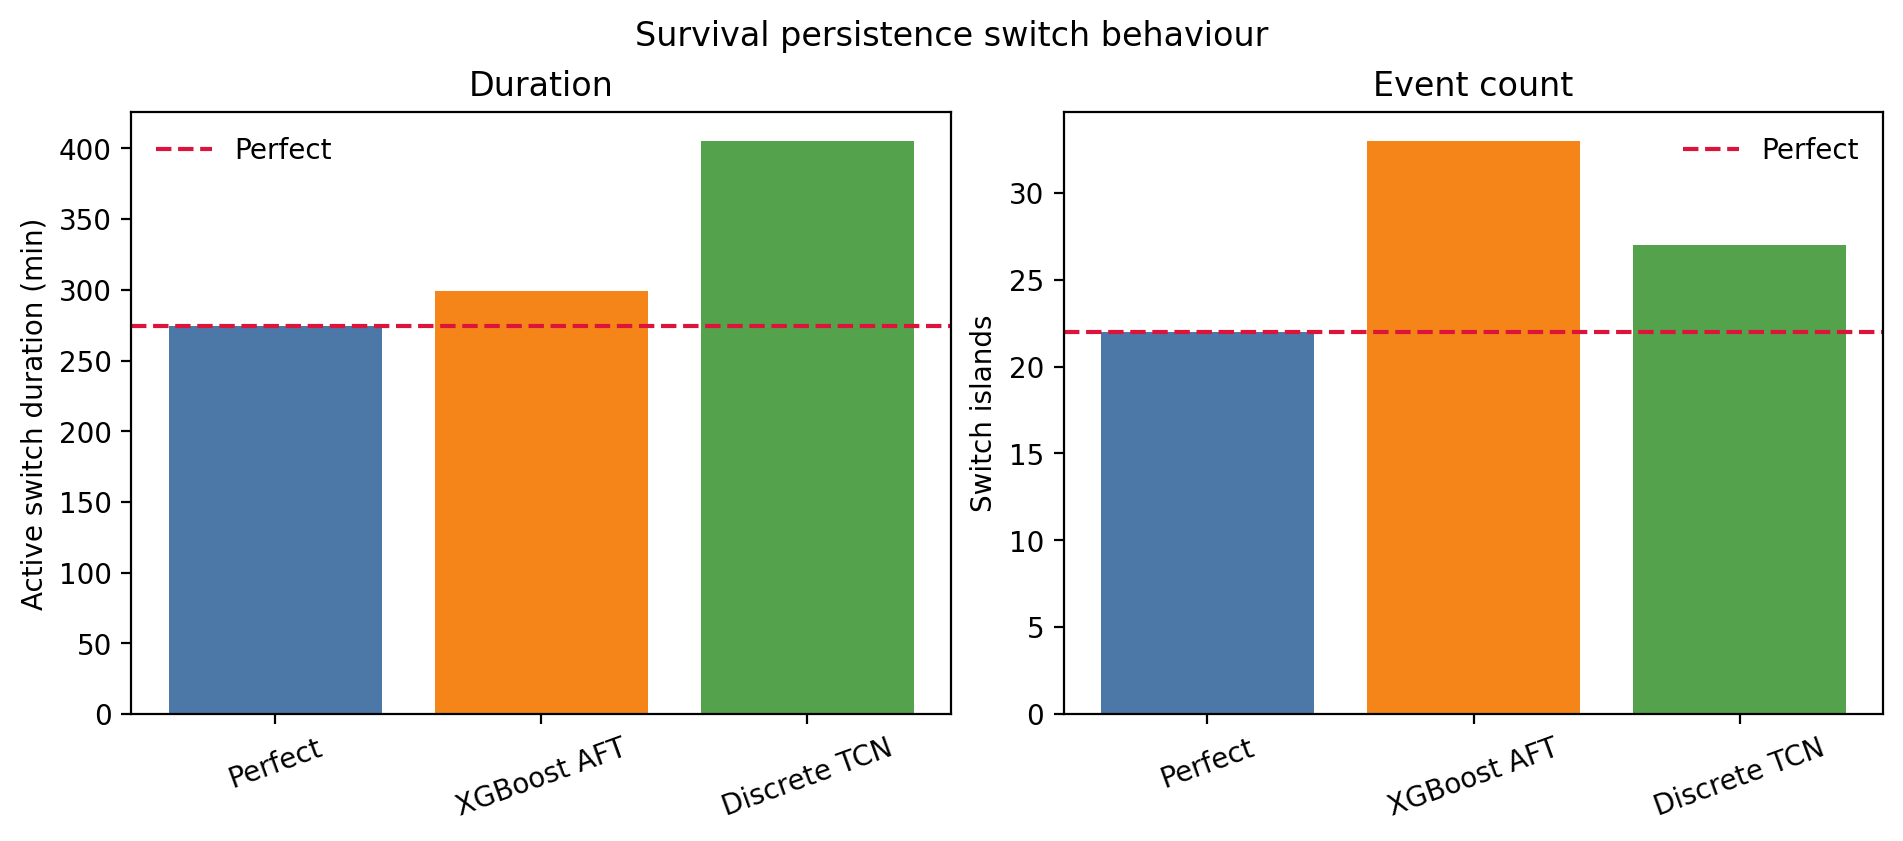
\includegraphics[width=0.82\textwidth]{results/survival_switch_duration_events.png}
  \caption{Survival persistence switch duration and event-count behavior on the external holdout split. Duration counts post-processed positive switch samples, converted to minutes using the \SI{30}{s} sampling time. The dashed red line marks the Perfect Switch value.}
  \label{fig:survival-switch-duration-events}
\end{figure}

\subsection{Interpretation and Event-Level Examples}
\label{sec:results-survival-examples}

\Cref{fig:survival-xgboost-switch-example} shows a false-positive example for
XGBoost-AFT on the task-native event \texttt{sp\_event\_00007}. This identifier
is local to the survival dataset and does not denote the event used in
\cref{fig:autoregressive-patchtst-switch-example,fig:current-level-xgboost-switch-example}.
On the 18 native decision timestamps, Perfect Switch is always zero, whereas
the final model switch is active for 12 samples. The example therefore
illustrates an unnecessary activation, not a successfully recovered reference
interval. The wider signal window also contains a later peak outside this
native event segment; the displayed switches are padded with zeros there and
must not be interpreted as predictions for that peak. This distinction matters
when interpreting task-native plots: only the native timestamps contribute to
the event metrics, while \cref{fig:cross-task-event-timeline} provides the
aligned cross-task view.

\begin{figure}[H]
  \centering
  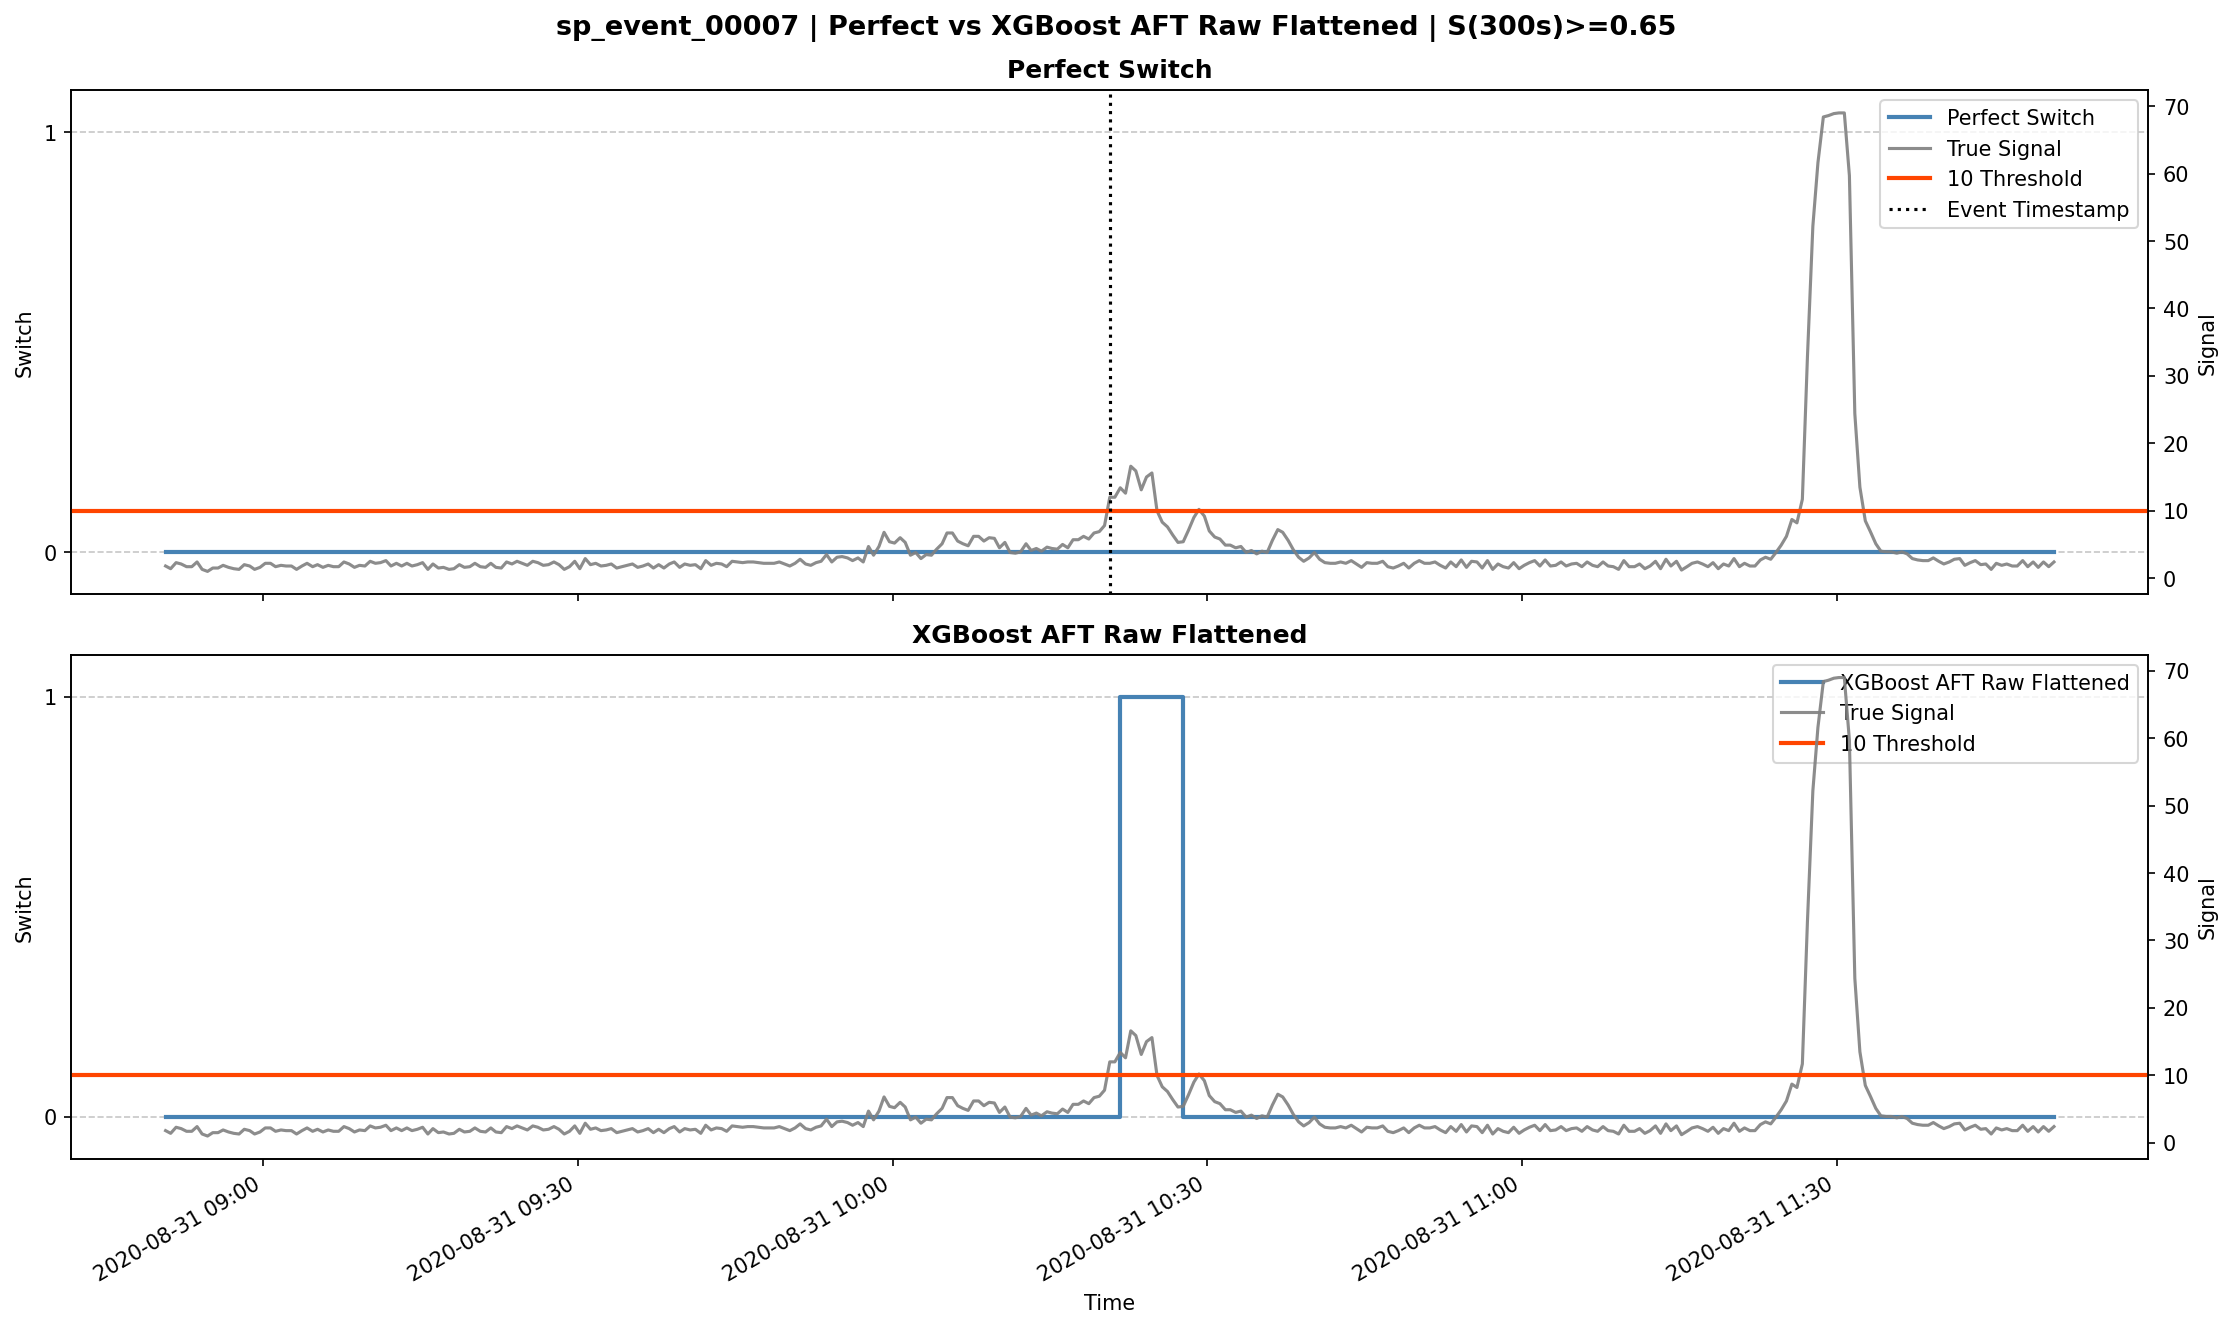
\includegraphics[width=0.92\textwidth]{results/survival_xgboost_aft_event_00007_switch_comparison.png}
  \caption[False-positive survival switch example for XGBoost-AFT.]{False-positive survival switch example for XGBoost-AFT on \texttt{sp\_event\_00007}. The model uses \(S(\SI{300}{s}\mid X_i)\geq 0.65\), the current-signal gate, and common post-processing. Perfect Switch remains zero on the native event; switches outside that segment are displayed as zero for context only.}
  \label{fig:survival-xgboost-switch-example}
\end{figure}

Overall, survival persistence is one of the most operationally meaningful
formulations because its output is a residual-duration distribution. In the
current experiments, XGBoost-AFT is the best survival switch model, while the
TCN provides better integrated probabilistic Brier performance but a less
precise binary switch sequence at the selected probability threshold.

\section{Cross-Task Switch Comparison}
\label{sec:results-cross-task-switch-comparison}

The previous sections compare models inside each task. A direct cross-task
comparison requires an additional alignment step, because the tasks do not make
decisions on exactly the same timestamps. The main comparison uses the common
Perfect Switch reference grid and treats missing native decisions as switch
\(0\). This is intentionally conservative: a method is penalized if its task
definition does not produce decisions over part of the reference grid. A second
strict-intersection comparison was also generated, but it is used only as a
diagnostic because it keeps only timestamps where all methods have native
decisions.

\Cref{tab:cross-task-best-results} reports the best method from each task on
the reference-grid comparison. Current-level XGBoost obtains the highest F1 and
perfect precision, but it does so with lower recall than the survival and
long-fade models. XGBoost-AFT is the strongest survival method and is close to
current-level XGBoost in F1 while reaching higher recall. Among autoregressive
models, PatchTST raw gives the best balance. Long-fade detection reaches full
recall, but its precision is lower because it keeps the switch active over a
larger part of grouped fade regions.

\begin{table}[htbp]
  \centering
  \caption{Best switch method from each task on the common reference grid. Missing native decisions are treated as switch \(0\).}
  \label{tab:cross-task-best-results}
  \small
  \setlength{\tabcolsep}{4pt}
  \renewcommand{\arraystretch}{1.15}
  \begin{tabular}{
    @{}
    >{\raggedright\arraybackslash}p{0.25\textwidth}
    >{\raggedright\arraybackslash}p{0.28\textwidth}
    rrrr
    @{}
  }
    \toprule
    Task & Best method
      & \shortstack{Coverage\\\(\uparrow\)}
      & \shortstack{Precision\\\(\uparrow\)}
      & \shortstack{Recall\\\(\uparrow\)}
      & \shortstack{F1\\\(\uparrow\)} \\
    \midrule
    Current-level persistence & XGBoost scalar context & 89.0\% & 1.000 & 0.808 & 0.894 \\
    Survival persistence & XGBoost-AFT & 9.2\% & 0.812 & 0.938 & 0.870 \\
    Autoregressive forecasting & PatchTST raw & 89.2\% & 0.779 & 0.821 & 0.800 \\
    Long-fade detection & TCN classifier & 28.7\% & 0.557 & 1.000 & 0.715 \\
    \bottomrule
  \end{tabular}
\end{table}

\Cref{fig:cross-task-f1-precision,fig:cross-task-recall-balanced-accuracy}
show the same comparison across all evaluated methods: F1 and precision in
the first figure, recall and balanced accuracy in the second. Both use the
same method order, ranked by F1. All values refer to the final switches after
the common island-removal and holding rules; raw model decisions are retained
only as diagnostics.

The F1 and precision panels highlight current-level XGBoost as the most
conservative useful method, with no false-positive switch samples on the
reference grid. PatchTST raw provides the strongest autoregressive balance.
However, precision alone does not show how much reference switch time is
missed, so these results must be read alongside recall.

The recall and balanced-accuracy panels show the other side of this trade-off.
Survival XGBoost-AFT recovers more reference switch time while keeping
precision relatively high. Long-fade detection models reach full or nearly full recall but
introduce extra switch duration, explaining their lower precision in
\cref{fig:cross-task-f1-precision}. The best model therefore depends on the
relative cost of missed coverage and unnecessary activation.

\begin{figure}[H]
  \centering
  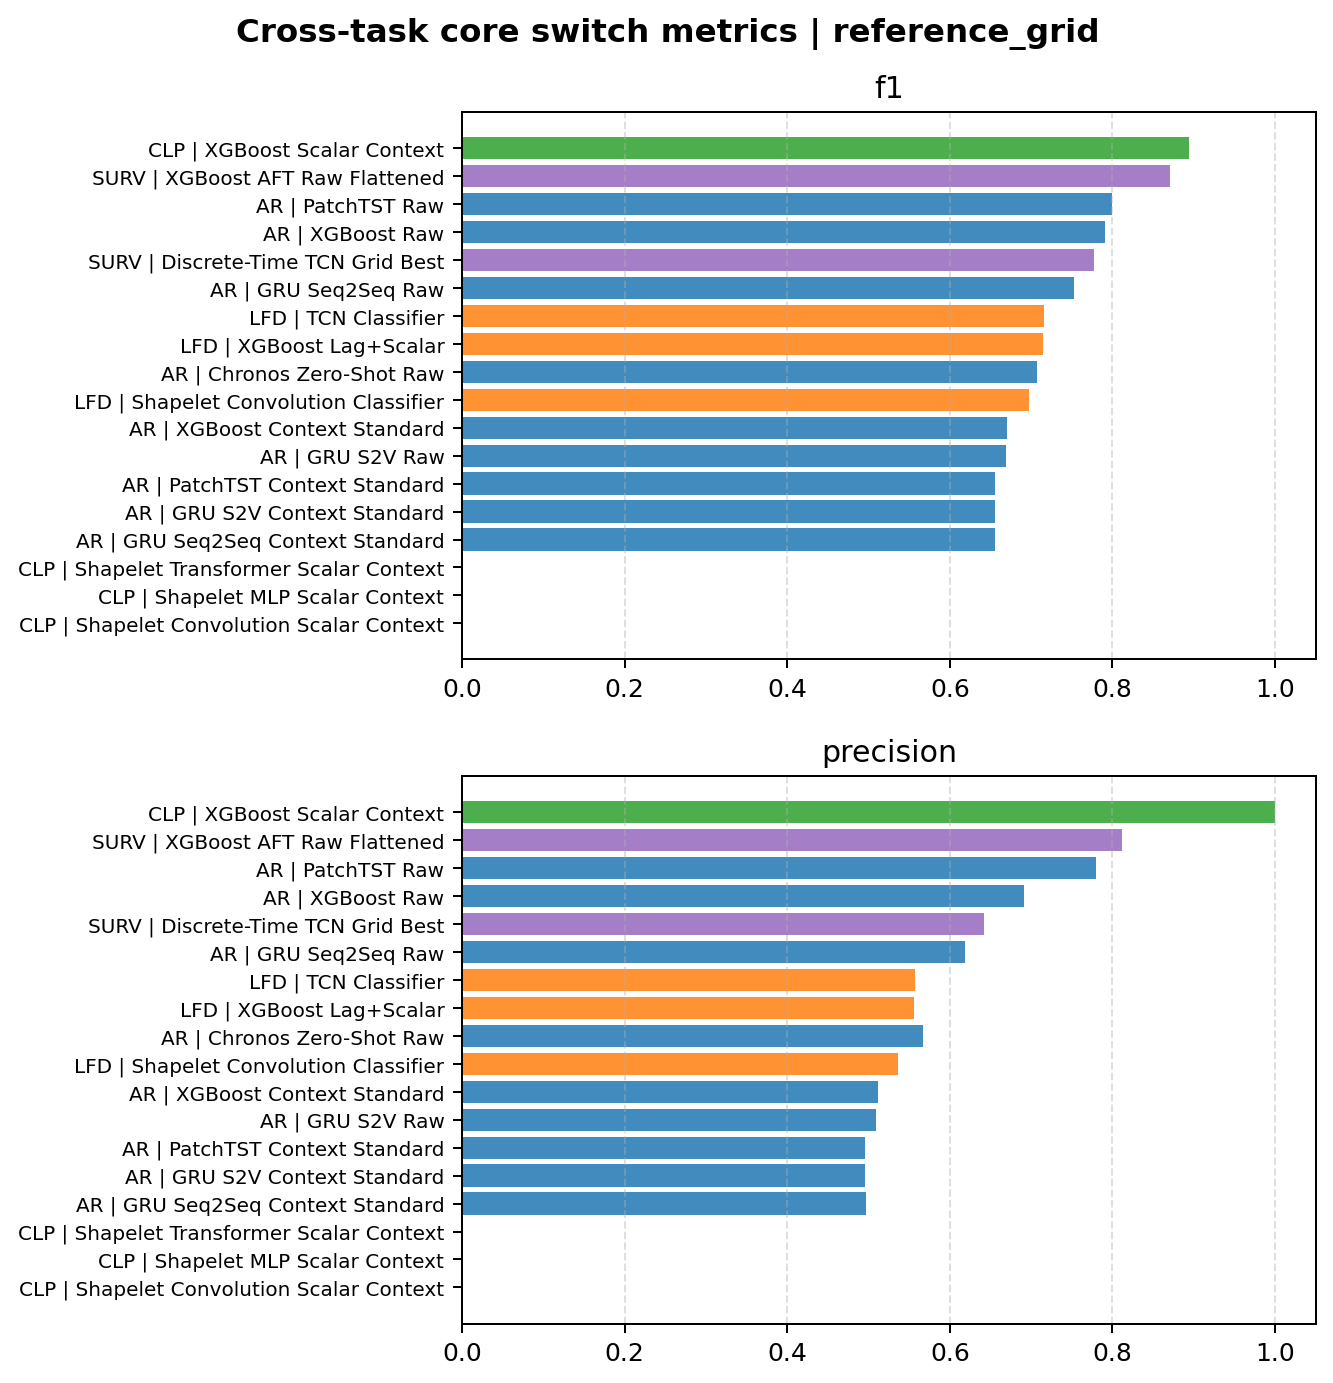
\includegraphics[width=\textwidth]{results/cross_task_reference_grid_f1_precision.png}
  \caption{Cross-task F1 (top) and precision (bottom) on the common reference grid. Missing native decisions are mapped to switch \(0\), so the comparison includes both decision quality and task coverage.}
  \label{fig:cross-task-f1-precision}
\end{figure}

\Cref{fig:cross-task-coverage} shows why native decision coverage is a critical
part of the interpretation. Autoregressive and
current-level models operate on most of the reference grid because their
datasets are based on candidate event windows. Long-fade detection is defined
only inside grouped fade events, and survival persistence is defined only while
the sample is inside a detected survival fade event.

\begin{figure}[H]
  \centering
  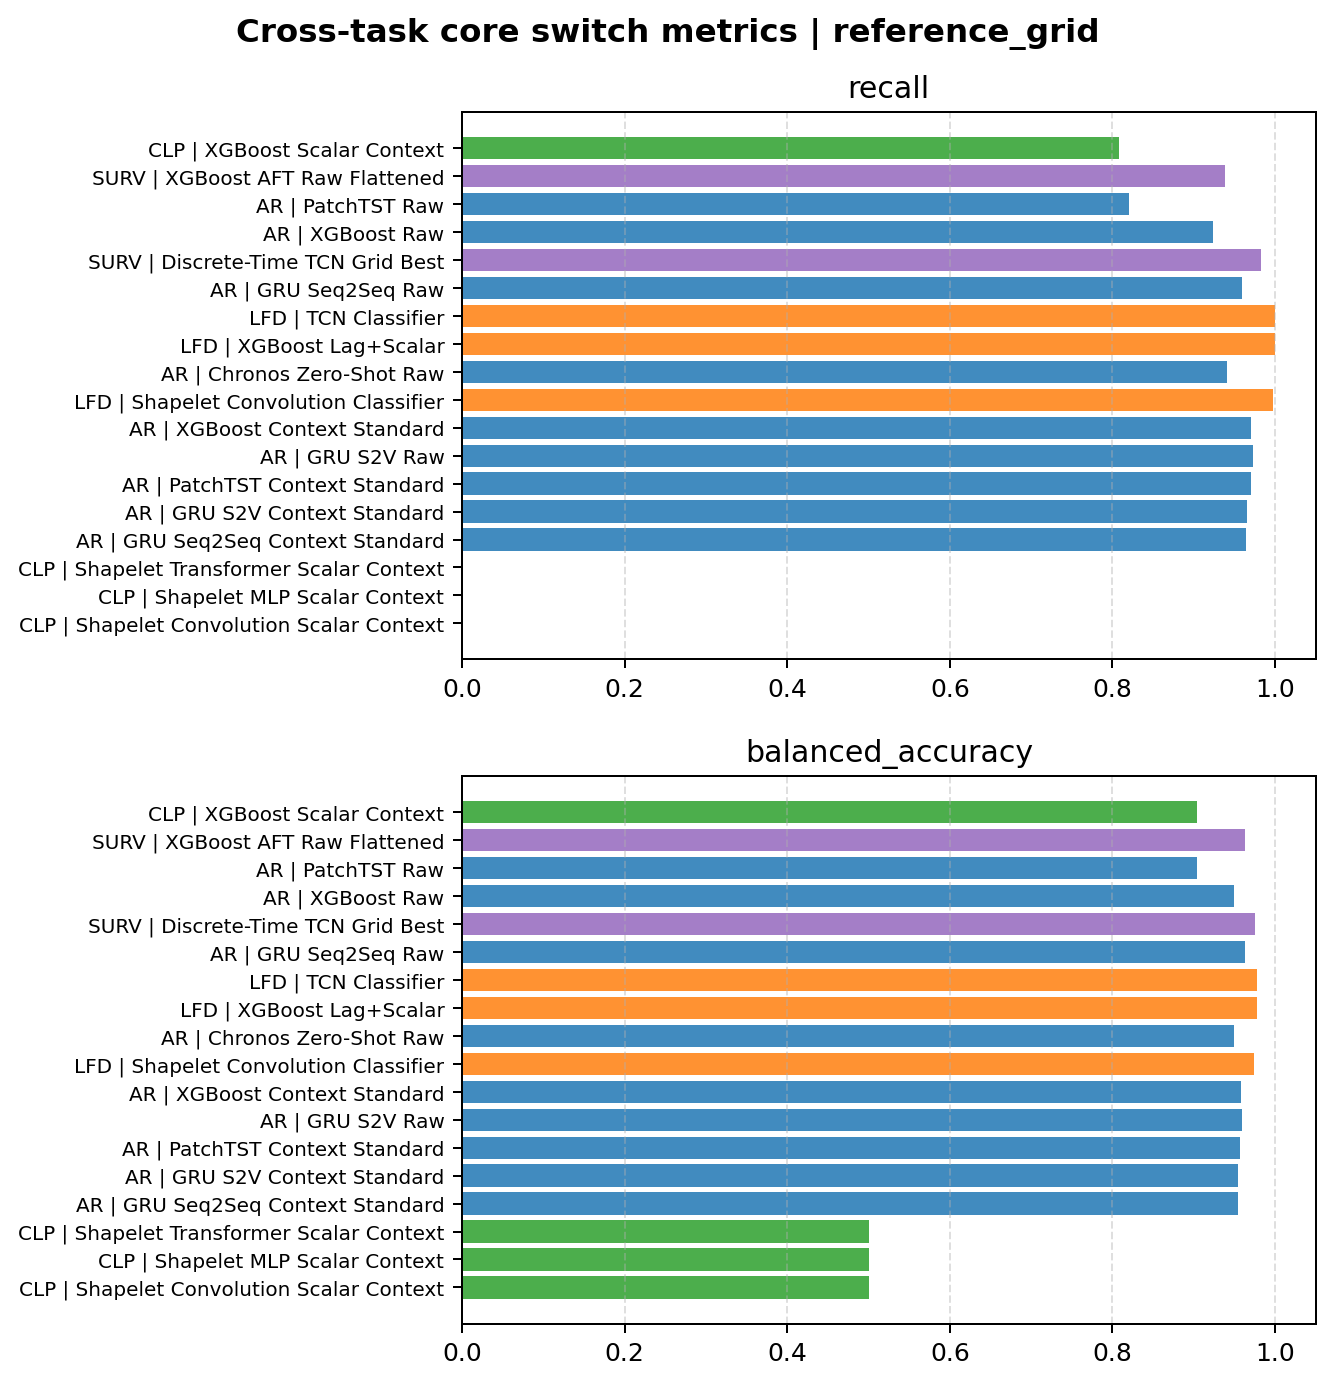
\includegraphics[width=\textwidth]{results/cross_task_reference_grid_recall_balanced_accuracy.png}
  \caption{Cross-task recall (top) and balanced accuracy (bottom) on the common reference grid, with the same method order and missing-decision policy as \cref{fig:cross-task-f1-precision}.}
  \label{fig:cross-task-recall-balanced-accuracy}
\end{figure}

Consequently, survival
metrics on the reference grid evaluate a smaller native decision domain, even
though the predictions are meaningful inside that domain.
The strict-intersection diagnostic removes this coverage effect by retaining
only the 771 timestamps where all task formulations provide native decisions.
On this reduced grid, current-level XGBoost remains the best conservative
method with precision \(1.000\), recall \(0.819\), and F1 \(0.900\).
XGBoost-AFT obtains precision \(0.814\), recall \(0.938\), and F1 \(0.872\),
and XGBoost raw is the strongest autoregressive method with F1 \(0.866\).

\begin{figure}[H]
  \centering
  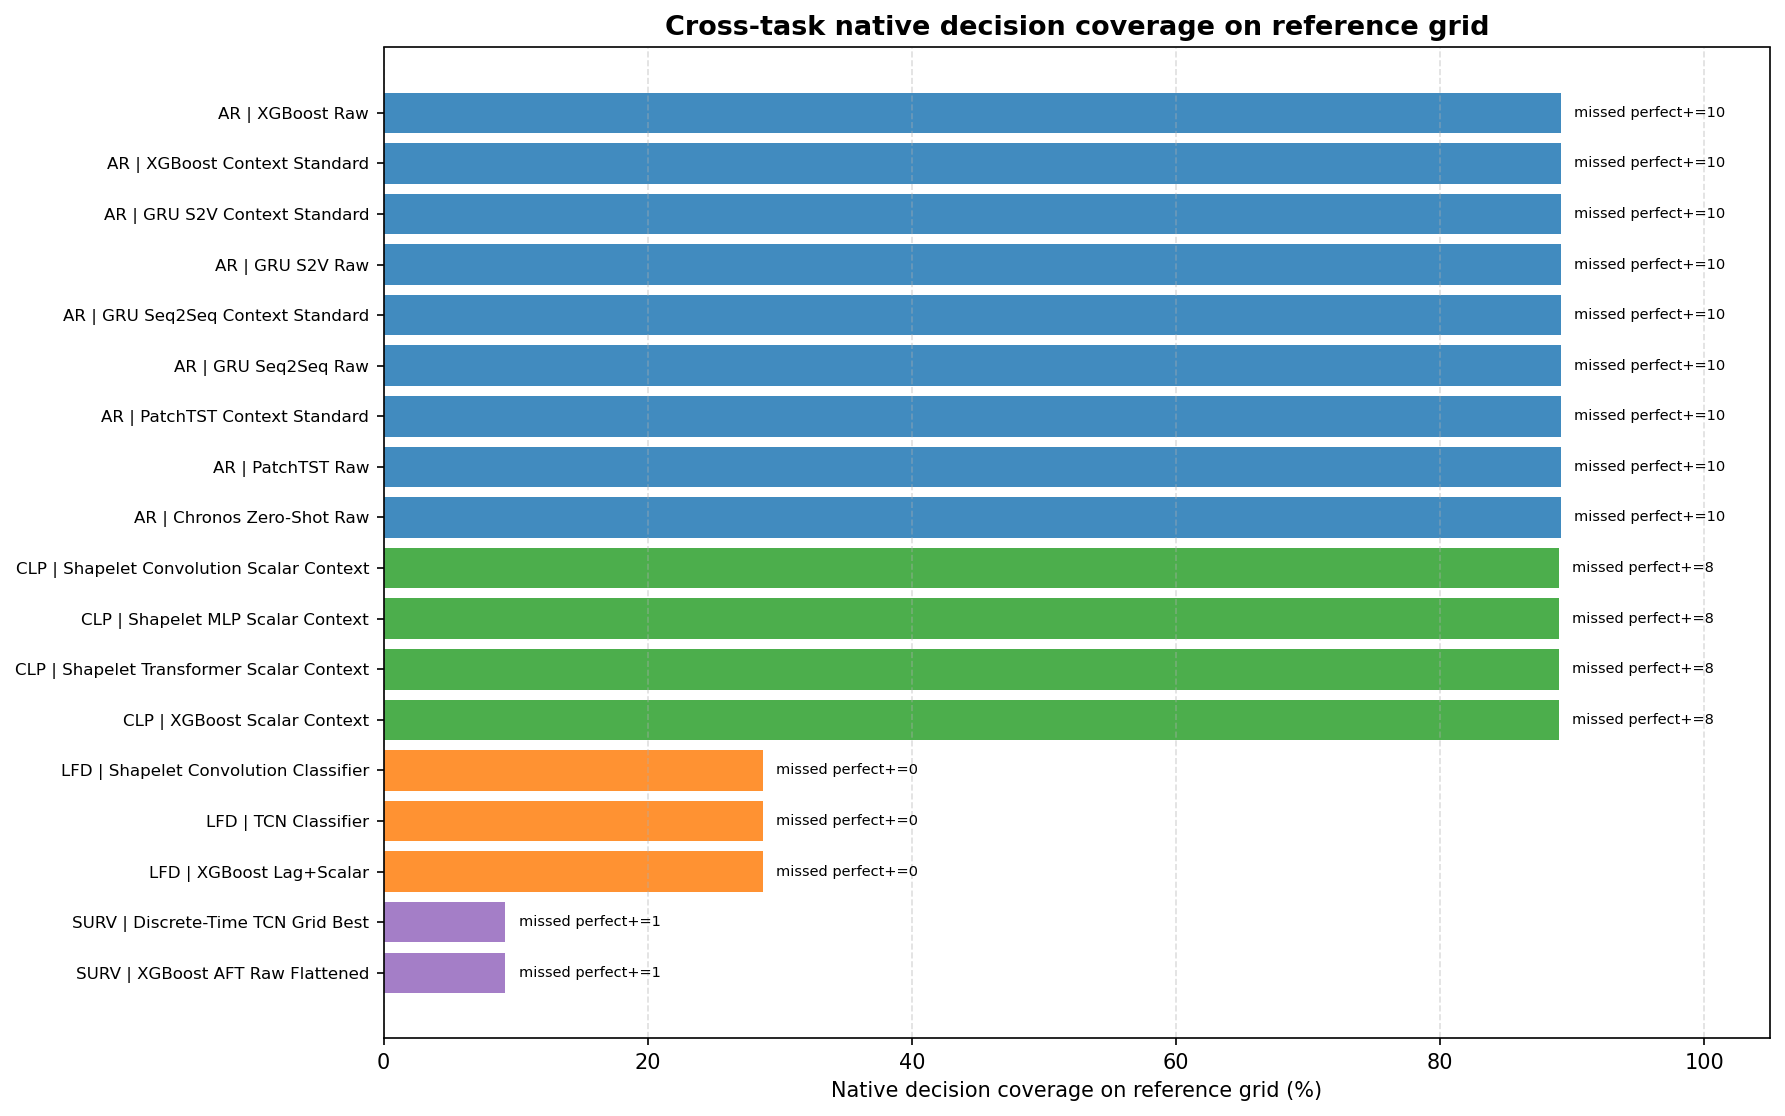
\includegraphics[width=1\textwidth]{results/cross_task_reference_grid_native_decision_coverage.png}
  \caption{Native decision coverage for each method on the common Perfect Switch reference grid. Lower coverage means that the corresponding task produces decisions on a smaller subset of reference timestamps.}
  \label{fig:cross-task-coverage}
\end{figure}


The long-fade TCN reaches recall \(1.000\) but only F1 \(0.778\). Therefore,
the main ranking is not only an artifact of missing decisions on the reference
grid: the same qualitative pattern remains when the comparison is restricted
to the shared native decision domain.

\Cref{fig:cross-task-event-f1-heatmap} reports event-level F1 values for the
selected reference events. The heatmap shows that no formulation dominates
uniformly. Some events are handled well by most models, while others expose
clear differences in onset timing, release timing, or excessive switch
activation. This supports the use of both global and event-level metrics:
global F1 summarizes average behavior, whereas event-level views reveal which
fade morphologies remain difficult.

The three all-zero rows corresponding to the current-level shapelet models are
genuine results rather than missing values or a coverage artifact. As discussed
in \Cref{sec:results-current-level-switch}, none of their test predictions
satisfies both the \SI{10.0}{dB} signal gate and the \SI{300}{s} predicted
persistence requirement. Their final switch sequence is therefore zero over
the complete test set. Every selected event containing a positive Perfect
Switch interval consequently has no true-positive shapelet decision and an
event-level F1 of zero. The heatmap makes explicit that this failure is
systematic across events, not confined to a few difficult fade morphologies.

\begin{figure}[H]
  \centering
  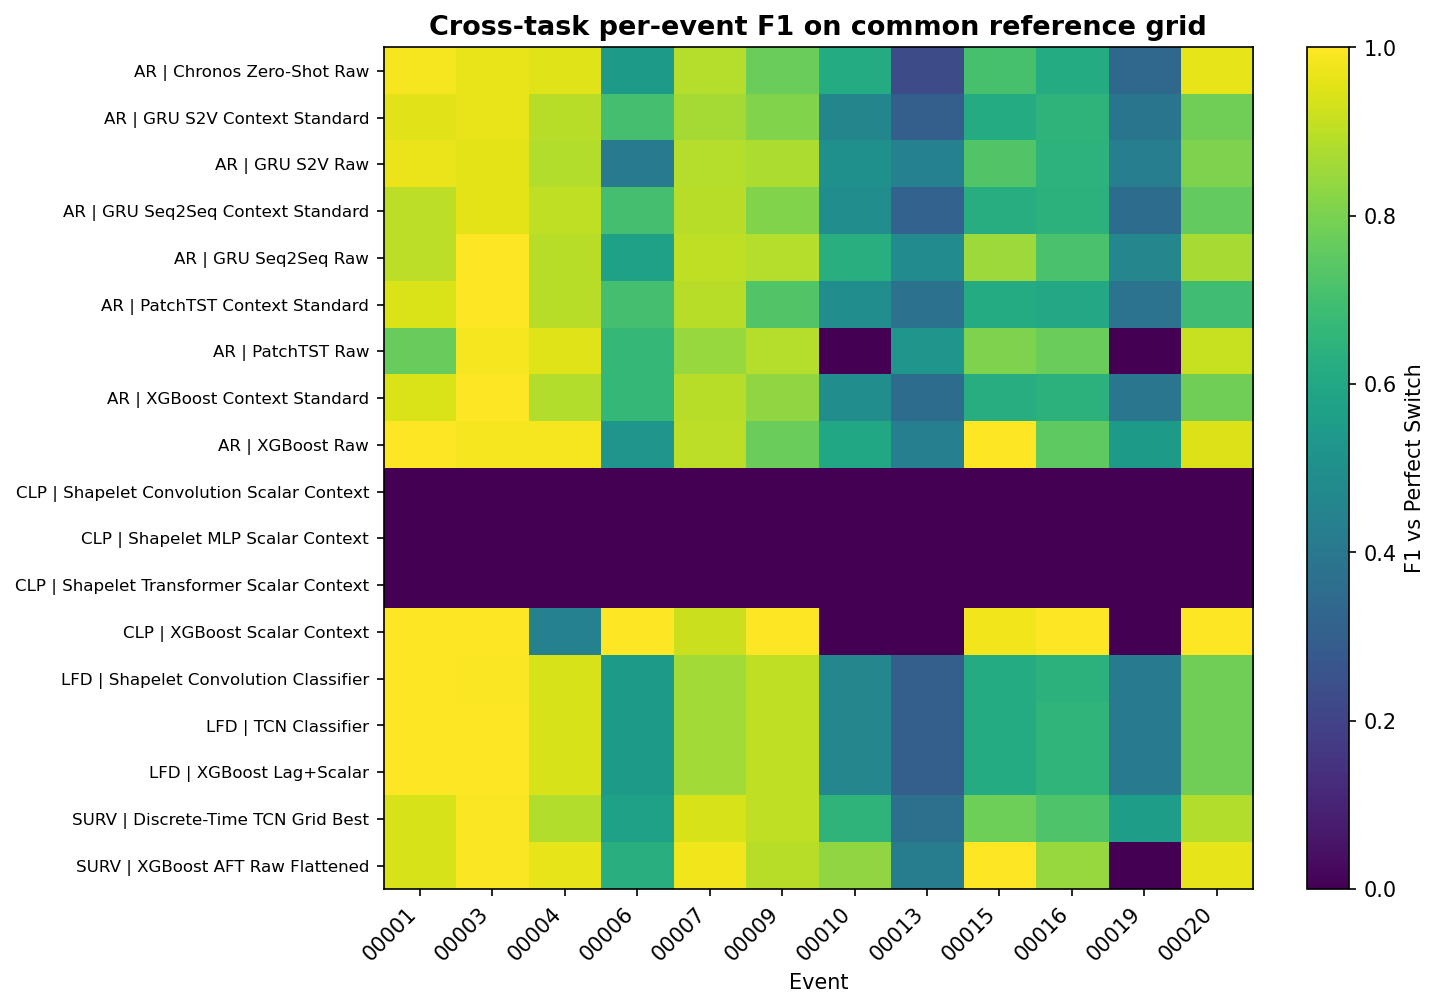
\includegraphics[width=\textwidth]{results/cross_task_reference_grid_event_f1_heatmap.png}
  \caption{Event-level F1 heatmap for the cross-task reference-grid comparison. Rows are model-derived switch methods and columns are selected external-holdout events.}
  \label{fig:cross-task-event-f1-heatmap}
\end{figure}

\Cref{fig:cross-task-event-timeline} gives a concrete example on a globally
aligned reference event, \texttt{dataset\_007\_event\_00007}, also used in
\cref{fig:autoregressive-patchtst-switch-example,fig:current-level-xgboost-switch-example}.
This is the figure to use when comparing methods from
different task formulations on exactly the same timestamps. The all-method
timeline makes the precision-recall trade-off visible: conservative models
activate later or for shorter intervals, while high-recall models cover more of
the fade but may extend beyond the Perfect Switch interval.

\begin{figure}[H]
  \centering
  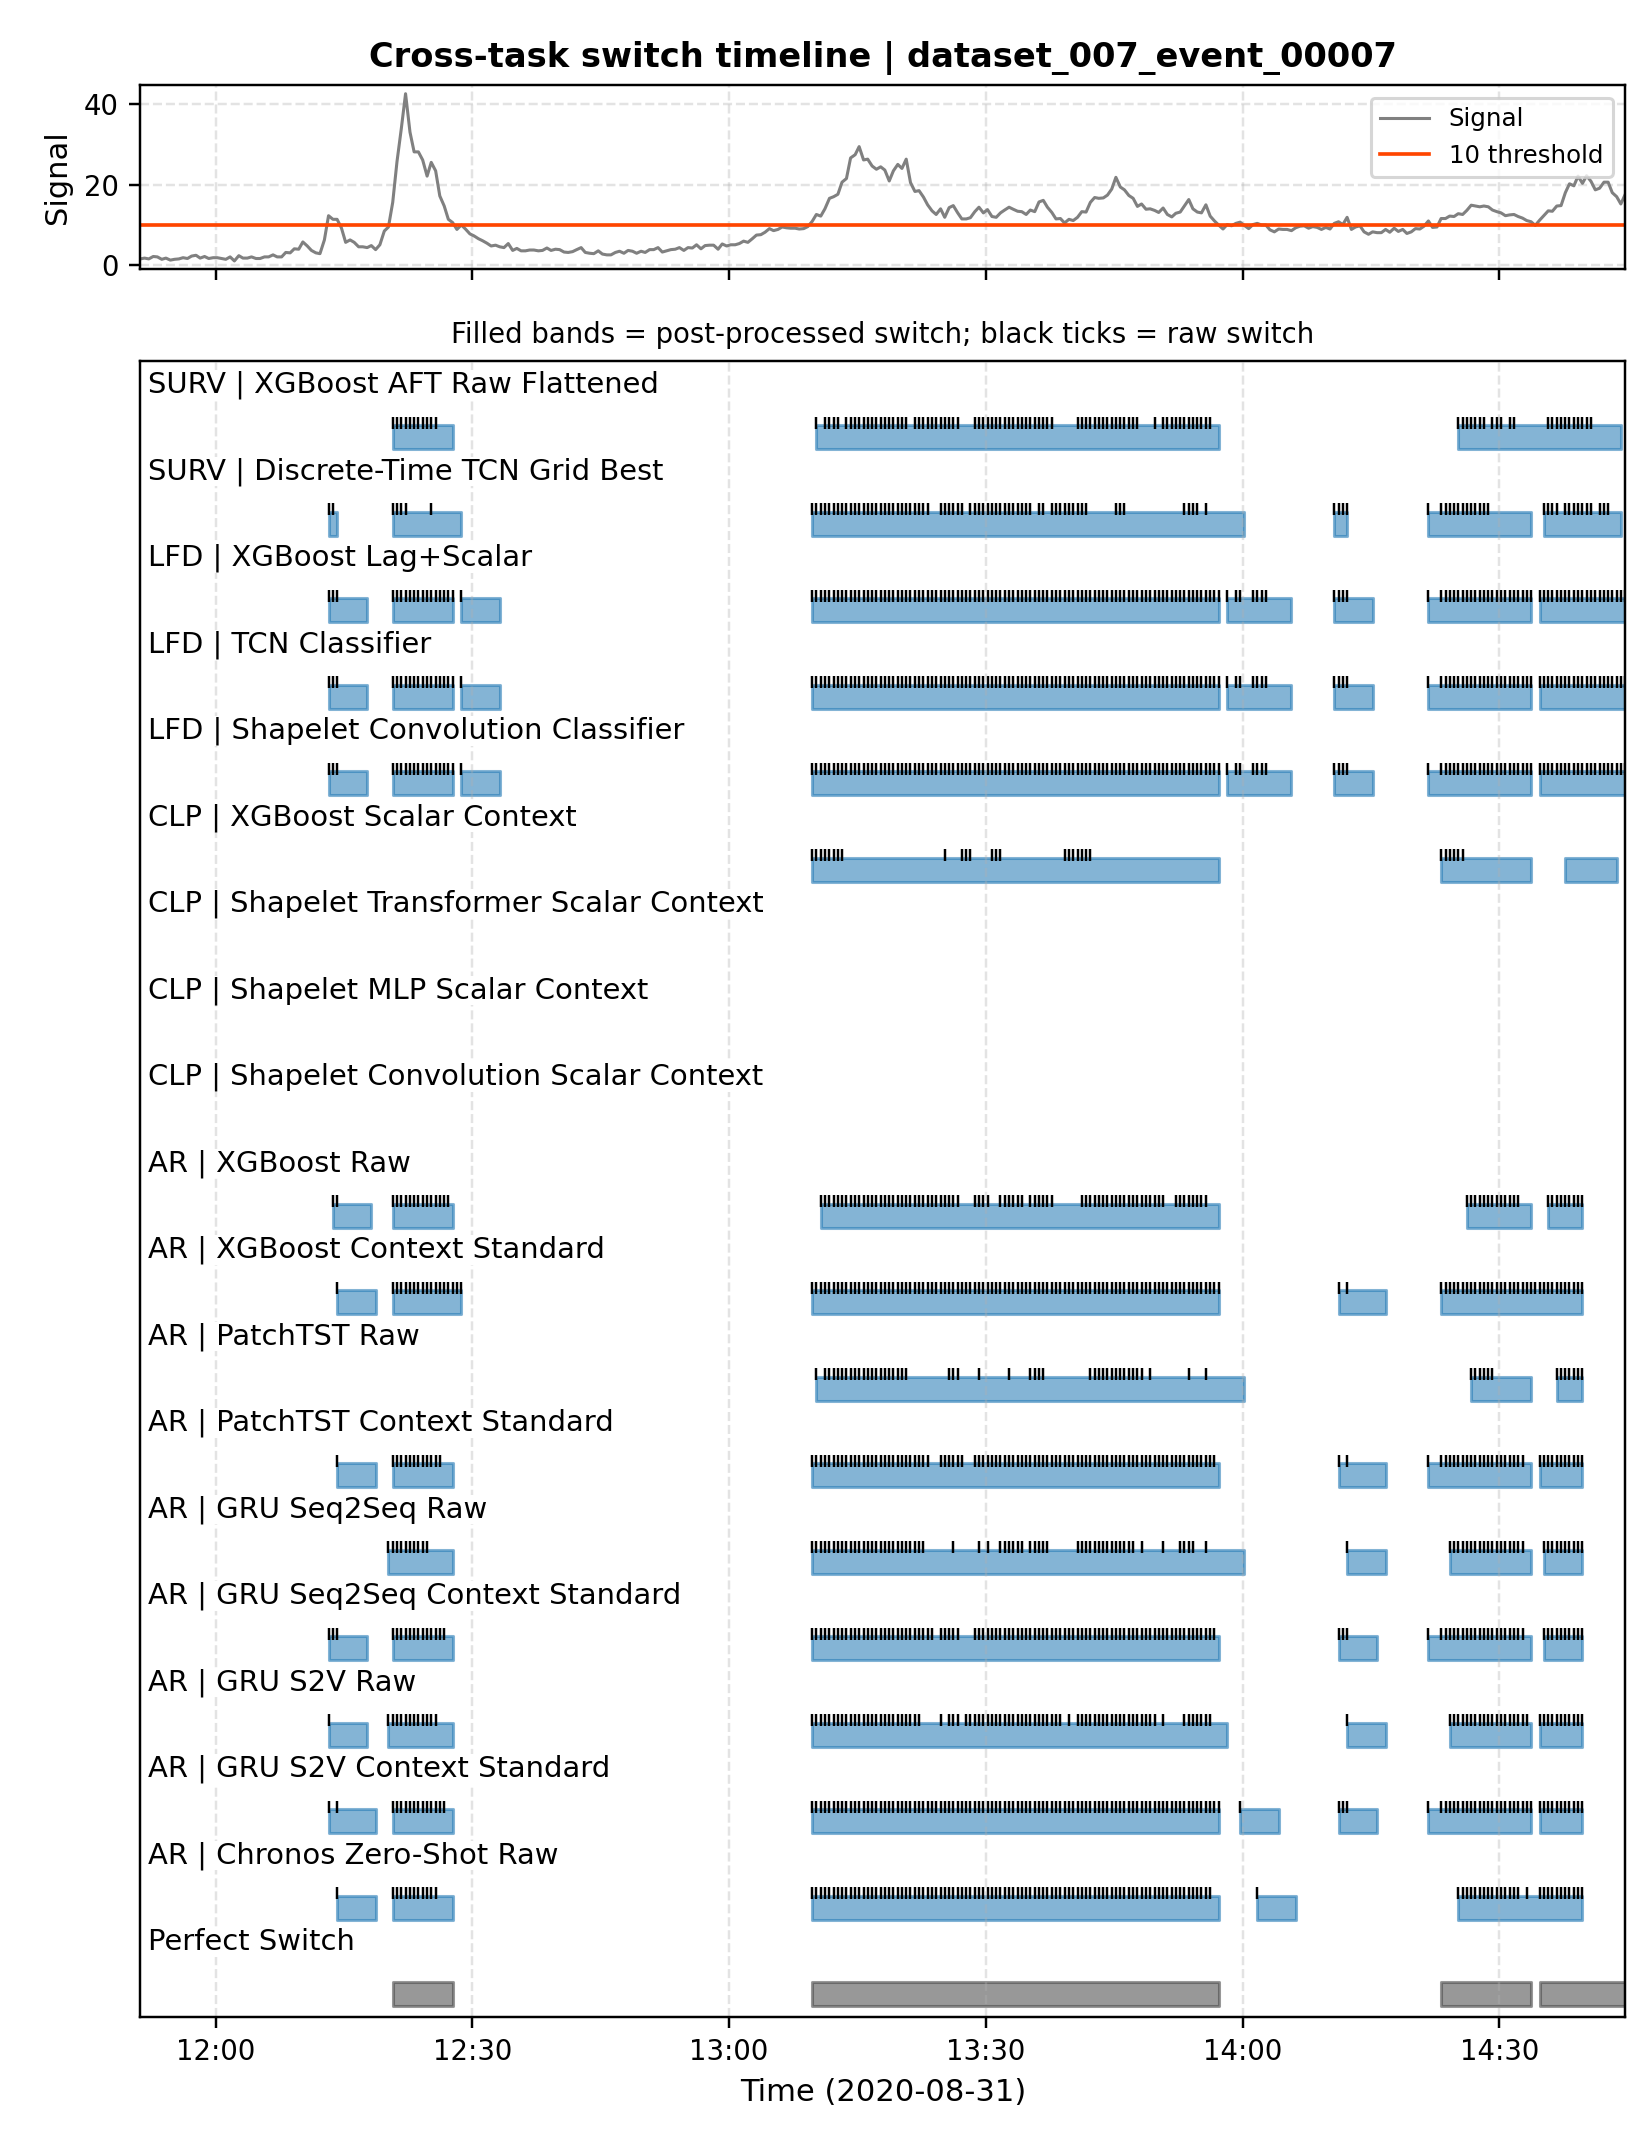
\includegraphics[width=1.0\textwidth]{results/cross_task_event00007_all_methods_switches.png}
  \caption{Cross-task event timeline for the selected multi-interval external-holdout event. The upper panel shows the raw signal and threshold. Each name labels the switch band immediately below it; filled bands show final post-processed decisions and black ticks show raw decisions.}
  \label{fig:cross-task-event-timeline}
\end{figure}

\section{Summary of Main Empirical Findings}
\label{sec:results-main-findings}

The experimental results lead to four main findings.

First, native predictive accuracy and switch quality are related but not
equivalent. In the autoregressive task, the raw GRU models obtain strong
forecast losses, but PatchTST raw gives the best switch F1 because its errors
produce a more useful threshold-crossing pattern. In survival persistence, the
discrete-time TCN has the best integrated Brier score, but XGBoost-AFT gives
the better switch sequence. In long-fade detection, near-perfect AUPRC does not
translate into a precise switch controller because the grouped-event label
overextends the active decision. These cases confirm that final evaluation
must be performed after switch conversion, not only in the native predictive
space.

Second, tabular gradient-boosted models are strong baselines. XGBoost is
competitive in autoregressive forecasting, is clearly the best current-level
persistence model, and XGBoost-AFT is the best survival switch model. This is
important methodologically: more complex neural sequence models are useful, but
they do not automatically dominate well-tuned lag and scalar representations on
this dataset.

Third, the different task formulations express different operating policies.
Current-level XGBoost is conservative and precise; survival XGBoost-AFT is a
strong residual-duration formulation with higher recall; PatchTST raw provides
the best autoregressive switch balance; long-fade detection is a robust
high-recall classifier but tends to overextend switch activity. The
learnable-shapelet current-level models are the clearest negative result: after
the operational conversion they never request a switch. These behaviors are
more informative than a single global ranking.

Fourth, the shared post-processing is essential for a fair operational
comparison. All final switch sequences are evaluated after the same island and
holding rules, and all are compared with the same Perfect Switch construction.
The remaining differences therefore come from the task formulation and model
outputs, not from task-specific switch logic. This also means that the reported
switch metrics should be read as operational metrics of the post-processed
decision sequence, not as metrics of the raw model threshold crossings.

Overall, the most promising formulations are current-level persistence with
XGBoost and survival persistence with XGBoost-AFT, followed by autoregressive
PatchTST raw. Current-level persistence gives the cleanest switch sequence in
the reported reference-grid comparison, but its underlying duration regression
has large tail errors. Survival persistence is conceptually closer to the
operational question because it estimates residual fade duration directly.
PatchTST raw remains valuable because it predicts the future signal trajectory
and can support analyses beyond the binary switch decision. Long-fade detection
is useful as a high-recall event classifier, but less precise as a standalone
switch controller.

\chapter{Conclusions}
\label{chap:conclusions}

Satellite fade nowcasting is useful when it supports timely switching, not
merely accurate intermediate predictions. The conclusions below identify what
the experiments establish about that objective and what remains unresolved.

\section{Contribution and Operational Lessons}

The contribution of this thesis is a decision-level comparison of four fade
nowcasting formulations, rather than a new model architecture. By mapping
different predictive outputs to a common switch reference and making decision
coverage explicit, the study distinguishes accurate intermediate predictions
from useful operational decisions. Its central empirical result is that the
best predictor according to a task's native loss is not necessarily the best
switch controller.

On the external holdout, current-level XGBoost, survival XGBoost-AFT, and raw
PatchTST produced useful but different switching policies: conservative
activation, higher fade coverage, and the strongest autoregressive switch
balance, respectively. These results support the use of signal-only models
for switching, but do not establish a universal winner.
In particular, the retained survival operating point was chosen exploratorily
on test data and still requires validation-only calibration.

The negative results are equally informative. The current-level shapelet
models never activated the switch on the evaluated test grid, while the
long-fade classifiers' strong classification scores did not prevent excessive
switch activity. Neither architectural complexity nor high native accuracy
was sufficient. The practical lesson is to select the predictive target and
assess its decision rule together: an output that is poorly aligned with the
required switch behavior cannot be judged useful from its native score alone.

\section{Answers to the Research Questions}

\paragraph{Can learned models improve switch decisions?}
The experiments support their usefulness: signal-history models can recover
reference switch intervals while limiting unnecessary activation. They do not,
however, establish superiority over a deployed engineering controller.
Well-tuned tabular models remained competitive with neural sequence models,
so greater architectural complexity is not itself evidence of operational
improvement.

\paragraph{Which formulation is most useful?}
The choice depends on the cost of missed fade coverage relative to unnecessary
switch time. Residual-duration survival modeling directly addresses whether an
ongoing fade will persist; current-level regression can support a conservative
policy but estimates a different quantity. Forecasting remains useful when
the future trajectory is also required. Grouped-event classification is better
suited to a high-recall warning than precise switch timing. These differences
make target definition an operational choice, not merely a modeling detail.

\paragraph{Do native metrics explain operational usefulness?}
Not sufficiently. The survival TCN obtained the better integrated Brier score,
whereas XGBoost-AFT produced the better switch sequence at the evaluated
operating point. Similarly, low forecast error did not identify the strongest
autoregressive switch model. Native scores remain necessary to assess the
predicted quantity, but decision timing, active duration, and fragmentation
must be assessed after conversion and post-processing.

\paragraph{Why are a common reference and post-processing necessary?}
They prevent differences in reference construction or decision smoothing from
being mistaken for model improvements. A common timestamp grid is also needed:
task-native scores alone compare decisions over different domains. Reporting
coverage alongside switch quality makes this distinction explicit and shows
where a method would still require a fallback decision in operation.

\section{Limitations}

The main limitation is the size and heterogeneity of the available data. The
external holdout design is stricter than a random split and is appropriate for
testing generalization, but it also means that the final conclusions are based
on one held-out acquisition source. Additional acquisition periods, terminals,
satellite links, and weather conditions would be needed to establish broader
operational robustness.

The thesis deliberately used a signal-only policy. This made the comparison
consistent across files and avoided dependence on columns that were not
available in all datasets. At the same time, it excluded potentially relevant
physical covariates, such as weather measurements, link geometry, or system
state variables. A model that combines signal history with consistently
available physical information could improve anticipation of fades, especially
before the signal crosses the operational threshold.

Another limitation concerns threshold and calibration choices. The switch
reference was built around a \SI{10.0}{dB} threshold and a
\SI{300}{s} operational duration. These values were fixed to make the
experiments comparable, but real deployments may prefer different operating
points. The survival probability threshold used for the retained switch
analysis was exploratory and not a fully validation-calibrated operating
point. Future work should calibrate all decision thresholds on validation data
only and then evaluate the chosen operating point on test data.

Finally, the cross-task comparison required aligning task-native decisions to a
common reference grid. This is necessary for fairness, but it also exposes a
structural issue: different task definitions do not naturally produce
decisions at exactly the same timestamps. The reported coverage values should
therefore be interpreted as part of the result, not as a nuisance. A task that
is accurate only on a small native domain may still be useful, but it cannot
replace a controller that must decide at every operational timestamp.

\section{Future Work}

The first extension should be validation-only calibration of switch-conversion
rules. Autoregressive trajectory thresholds, current-level duration
thresholds, long-fade probability thresholds, and survival probability
thresholds should be tuned on validation data using explicitly chosen
operational costs. This would turn the current comparison from a fixed-rule
benchmark into a calibrated decision study.

Second, the survival formulation should be developed further. XGBoost-AFT
showed that residual-duration modeling is promising, but richer survival
models could improve calibration and event-level timing. Candidate directions
include better discrete-time neural survival models, DeepHit-style competing
risk formulations if multiple event types are introduced, and validation of
survival probability calibration across operational horizons.

Third, the dataset should be expanded and enriched. More external holdout
sources would allow blocked or source-level cross-validation, reducing the risk
that the conclusions depend on one held-out file. If auxiliary variables become
available consistently, future work could compare the current signal-only
framework with a physically enriched framework while preserving the same
no-leakage and switch-evaluation protocol.

Fourth, future experiments should connect the switch metrics to explicit
operational costs. Precision, recall, F1, IoU, active duration, and event
counts describe different aspects of switch behavior, but an operator may
assign asymmetric costs to false activations, missed fades, delayed onsets, and
excessive switch fragmentation. A cost-based decision layer would make the
choice between conservative and high-recall models more transparent.

Fifth, the framework should be moved from offline evaluation toward an online
nowcasting prototype. The current experiments reproduce the information
available at each decision time, but they are still executed as batch analyses.
A deployable system would need streaming ingestion, stateful preprocessing,
incremental gap and quality checks, stateful switch post-processing, latency
measurement, and clear fallback behavior when input quality is poor. Such a
prototype would also make it possible to compare the learned decision rules
against engineering baselines under realistic operating constraints, rather
than only after the acquisition has been processed offline.

The broader conclusion is that satellite fade nowcasting should be treated as a
decision-oriented time-series problem. Accurate forecasts, duration estimates,
and survival curves are valuable only insofar as they support timely and
reliable switch decisions. The framework developed in this thesis provides a
reproducible basis for that evaluation and shows that task formulation,
post-processing, and operational metrics are central components of the
modeling problem, not secondary details.


\appendix
\chapter{Implementation Details}
\label{app:implementation-details}

This appendix summarizes implementation details that are useful for
reproducing the experiments but would interrupt the main methodological
discussion. The repository was organized so that each task has its own
configuration files, dataset builder, model runners, saved model artifacts, and
result folders, while sharing common preprocessing, switch construction, and
evaluation utilities.

\section{Repository Structure}
\label{app:repository-structure}

The codebase separates common infrastructure from task-specific logic. Common
utilities live under \path{src/data/}, \path{src/switching/}, \path{src/utils/},
and \path{src/tuning/}. Task-specific implementations live under
\path{src/tasks/<task_name>/}. Experiment entry points are grouped in
\path{scripts/experiments/<task_name>/}, while analysis and comparison scripts
are grouped in \path{scripts/analysis/}.

\Cref{tab:appendix-repo-structure} gives the practical role of the main
repository folders. The table is intended as a reproducibility map: it shows
where configuration, immutable raw data, intermediate preprocessing outputs,
final model-ready datasets, fitted models, and result artifacts are stored.

\begin{table}[htbp]
  \centering
  \caption{Main repository folders used by the experimental pipeline.}
  \label{tab:appendix-repo-structure}
  \small
  \setlength{\tabcolsep}{4pt}
  \renewcommand{\arraystretch}{1.15}
  \begin{tabular}{
    @{}
    >{\raggedright\arraybackslash}p{0.30\textwidth}
    >{\raggedright\arraybackslash}p{0.62\textwidth}
    @{}
  }
    \toprule
    Folder & Purpose \\
    \midrule
    \path{configs/}
      & YAML configuration files for data preparation, model runs, grid searches, Perfect Switch construction, and switch comparisons. \\
    \path{data/raw/}
      & Original input files. These files are treated as read-only. \\
    \path{data/interim/}
      & Cleaned signals, candidate events, event windows, and intermediate reusable preprocessing artifacts. \\
    \path{data/processed/}
      & Final task-specific arrays and metadata used by model runners. \\
    \path{src/tasks/}
      & Task-scoped dataset, model, evaluation, plotting, and utility code. \\
    \path{src/switching/}
      & Model-agnostic Perfect Switch, switch conversion, post-processing, metrics, and plotting utilities. \\
    \path{scripts/experiments/}
      & Executable training, zero-shot evaluation, dataset-building, and grid-search scripts. \\
    \path{scripts/analysis/}
      & Data-analysis and post-training comparison scripts. \\
    \path{models/}
      & Saved checkpoints, fitted estimators, model configurations, and run metadata. \\
    \path{results/}
      & Predictions, metrics, tables, figures, comparison summaries, and result indexes. \\
    \bottomrule
  \end{tabular}
\end{table}

The main task namespaces are \path{autoregressive},
\path{current_level_persistence}, \path{long_fade_detection}, and
\path{survival_persistence}. This separation avoids storing task-specific
models or outputs under a generic folder and makes it possible to trace every
result back to its task formulation.

\section{Dataset Artifact Schema}
\label{app:dataset-artifact-schema}

Every processed dataset is stored together with metadata describing the
selection identifier, split definition, context length, threshold assumptions,
and preprocessing fingerprint. The canonical split is development versus
external holdout: training and validation are drawn from development sources,
whereas \path{fc-uplink-fade.csv} is used only as the final test source.

\Cref{tab:appendix-dataset-artifacts} summarizes the arrays and metadata saved
by each task-specific dataset builder. The table separates numerical arrays
from metadata because the metadata is required to align predictions back to
timestamps, events, source datasets, and switch-evaluation windows.

\begin{table}[htbp]
  \centering
  \caption{Main processed dataset artifacts by task.}
  \label{tab:appendix-dataset-artifacts}
  \small
  \setlength{\tabcolsep}{3pt}
  \renewcommand{\arraystretch}{1.15}
  \begin{tabular}{
    @{}
    >{\raggedright\arraybackslash}p{0.23\textwidth}
    >{\raggedright\arraybackslash}p{0.33\textwidth}
    >{\raggedright\arraybackslash}p{0.34\textwidth}
    @{}
  }
    \toprule
    Task & Array artifacts & Metadata artifacts \\
    \midrule
    Autoregressive forecasting
      & \path{train.npz}, \path{val.npz}, and \path{test.npz} with raw and context-standardized past windows and future trajectories.
      & Split metadata parquet files with window identifiers, event identifiers, source dataset names, timestamps, quality flags, and scaling parameters. \\
    Current-level persistence
      & Split NPZ files with raw context, relative-to-current context, scalar context features, and persistence duration targets.
      & Metadata with target duration, censoring flags, acquisition segment identifiers, scalar feature names, and train-only scaler parameters. \\
    Long-fade detection
      & Split NPZ files with sequence context, relative-to-threshold context, scalar context, and binary long-fade labels.
      & Metadata with grouped-event identifiers, event labels, timestamps, dataset identifiers, and quality flags. \\
    Survival persistence
      & Split NPZ files with past contexts, scalar features, residual-duration labels, and AFT lower/upper bounds.
      & Metadata with event identifiers, censoring indicators, acquisition segment identifiers, observed durations, and survival target bounds. \\
    \bottomrule
  \end{tabular}
\end{table}

The split metadata is as important as the numerical arrays. It preserves the
alignment between model inputs, event timestamps, source files, event
identifiers, and later switch comparisons. Model scripts do not reconstruct
splits independently; they load these artifacts and validate their fingerprints
where necessary.

\section{Run and Result Artifact Schema}
\label{app:run-result-artifact-schema}

Each trained or evaluated model writes a run folder under
\path{results/runs/<task_name>/} and, when applicable, a model folder under
\path{models/<task_name>/}. Run identifiers encode the task, model family,
variant, selection identifier, and relevant setup. A typical run folder
contains:

\begin{itemize}
  \item \path{predictions/}: validation and/or test predictions in parquet
  format;
  \item \path{metrics/}: native task metrics such as forecast errors,
  classification scores, duration errors, or survival metrics;
  \item \path{figures/}: diagnostic plots generated by the run;
  \item \path{tables/}: compact run summaries;
  \item \path{metadata.yaml}: configuration, dataset fingerprint, selected
  device, seed, and file paths.
\end{itemize}

Switch comparisons are stored separately from native model runs because the
same predictions can be converted into switch sequences under different
decision rules. Model-vs-reference comparisons are written under
\path{results/comparisons/switch_eval/<task_name>/<selection_id>/}. Cross-task
comparisons are written under
\path{results/comparisons/cross_task_switch/<selection_id>/}. This separation
keeps model training artifacts distinct from downstream operational
evaluation.

\section{Reproducibility Checklist}
\label{app:reproducibility-checklist}

The experiments are intended to be reproducible from configurations and saved
artifacts. The following information is recorded or fixed for each run:

\begin{itemize}
  \item the YAML configuration path and configuration fingerprint;
  \item the processed dataset path and dataset metadata fingerprint;
  \item the task formulation, input representation, target definition, context
  length, prediction horizon or duration horizon, and threshold assumptions;
  \item train, validation, and external test split metadata;
  \item random seed and hardware device used by the model runner;
  \item model hyperparameters, selected validation score, and final test
  metrics;
  \item saved predictions used for switch conversion;
  \item switch-conversion rule, post-processing settings, and Perfect Switch
  reference path.
\end{itemize}

The Python environment is specified by \path{environment.yml}. Experiments use
the active environment rather than creating a new virtual environment inside
the repository. GPU acceleration is used when available, with CUDA preferred,
then Apple MPS when supported, and CPU as a fallback. Grid searches distribute
independent trials over available CUDA devices when possible.

\chapter{Hyperparameter Grids}
\label{app:hyperparameter-grids}

This appendix reports the configurations selected by the validation-only
model-selection searches summarized in \cref{sec:hyperparameter-search}. The
tables list the archived selection score used by each search. Final external
test metrics and switch metrics are reported in \cref{chap:results}; they should
be considered the primary performance results.

For current-level persistence, some duration metrics were refreshed without
retraining after dataset-alignment updates. The configurations below are the
selected model artifacts; the refreshed validation and test metrics used for
the final discussion are those in \cref{chap:results}.

\section{Search Design Summary}

\Cref{tab:appendix-grid-search-summary} summarizes the model-selection
searches used in the thesis. All searches use validation-only criteria. The
external holdout split is not used to choose hyperparameters, thresholds, or
checkpoints.
The purpose of this table is to make the scale of the model-selection phase
explicit before listing the selected configurations. It reports the criterion
used to rank trials, the number of evaluated trials, and the main
hyperparameter families varied by each search.

\begin{table}[htbp]
  \centering
  \caption{Summary of the hyperparameter searches. Trial counts refer to the archived searches used for the reported model artifacts.}
  \label{tab:appendix-grid-search-summary}
  \scriptsize
  \setlength{\tabcolsep}{3pt}
  \renewcommand{\arraystretch}{1.15}
  \begin{tabular}{
    @{}
    >{\raggedright\arraybackslash}p{0.20\textwidth}
    >{\raggedright\arraybackslash}p{0.22\textwidth}
    >{\raggedright\arraybackslash}p{0.18\textwidth}
    >{\raggedleft\arraybackslash}p{0.08\textwidth}
    >{\raggedright\arraybackslash}p{0.23\textwidth}
    @{}
  }
    \toprule
    Task & Search & Selection criterion & Trials & Main varied hyperparameters \\
    \midrule
    Autoregressive
      & GRU S2V and encoder-decoder, raw and context-standard variants
      & validation RMSE, minimized
      & 576
      & hidden size, number of layers, learning rate, weight decay, teacher forcing, architecture. \\
    Autoregressive
      & PatchTST, raw and context-standard variants
      & validation RMSE, minimized
      & 1728
      & patch length, stride, model dimension, attention heads, number of layers, dropout, learning rate. \\
    Autoregressive
      & XGBoost multi-output horizon regressors
      & validation RMSE, minimized
      & 2304
      & number of trees, depth, learning rate, subsampling, column sampling, minimum child weight, \(L_2\) regularization. \\
    Current-level persistence
      & Learnable-shapelet MLP, Transformer, and convolution heads
      & validation MAE in seconds, minimized
      & 648
      & shapelet count, hidden dimensions, scalar encoder size, depth, dropout, learning rate. \\
    Current-level persistence
      & XGBoost duration regressor
      & validation MAE in seconds, minimized
      & 1152
      & number of trees, depth, learning rate, subsampling, column sampling, minimum child weight, \(L_2\) regularization. \\
    Long-fade detection
      & XGBoost, TCN, and shapelet-convolution classifiers
      & validation AUPRC, maximized
      & 8928
      & tree parameters, TCN channels/depth/kernel/dropout, shapelet count/lengths, scalar hidden dimension, learning rate, batch size. \\
    Survival persistence
      & XGBoost-AFT
      & validation AFT negative log-likelihood, minimized
      & 1920
      & input representation, sample weighting, AFT distribution, AFT scale, tree depth, learning rate, subsampling, column sampling, regularization. \\
    Survival persistence
      & Discrete-time TCN
      & validation integrated Brier score, minimized
      & 1620
      & binning strategy, input representation, sample weighting, channel schedule, kernel size, dropout, learning rate, weight decay, batch size. \\
    \bottomrule
  \end{tabular}
\end{table}

For tree-based grids, the configuration files use explicit numeric ranges
defined by start, stop, and step values. For neural grids, categorical lists are
used for architecture choices such as hidden dimensions, layer counts, dropout
values, and learning rates. The resulting trial tables are archived under
\path{results/grid_searches/}; the tables below report only the selected
configuration for each model family or variant.

\section{Autoregressive Forecasting}

The autoregressive searches are run separately for the raw and
context-standardized variants. Chronos is excluded from this table because it
is evaluated in zero-shot mode and no hyperparameters are fitted.
\Cref{tab:appendix-ar-best-configs} reports the best validation-selected
configuration for each trainable autoregressive model and input variant. The
selection score is the validation RMSE on the raw signal scale; the external
test metrics are discussed in the results chapter rather than repeated here.

\begin{table}[htbp]
  \centering
  \caption{Best validation-selected autoregressive configurations.}
  \label{tab:appendix-ar-best-configs}
  \scriptsize
  \setlength{\tabcolsep}{3pt}
  \renewcommand{\arraystretch}{1.18}
  \begin{tabular}{
    @{}
    >{\raggedright\arraybackslash}p{0.17\textwidth}
    >{\raggedright\arraybackslash}p{0.13\textwidth}
    >{\raggedright\arraybackslash}p{0.48\textwidth}
    >{\raggedleft\arraybackslash}p{0.14\textwidth}
    @{}
  }
    \toprule
    Model & Variant & Selected configuration & Validation RMSE \\
    \midrule
    GRU S2V & raw
      & hidden size 16; 1 layer; learning rate 0.001; weight decay 0; teacher forcing 0
      & 5.520 \\
    GRU S2V & context-standard
      & hidden size 64; 1 layer; learning rate 0.001; weight decay 0.0001; teacher forcing 0
      & 3.716 \\
    GRU encoder-decoder & raw
      & hidden size 64; 1 layer; learning rate 0.001; weight decay 0.0001; teacher forcing 0.5
      & 4.023 \\
    GRU encoder-decoder & context-standard
      & hidden size 64; 3 layers; learning rate 0.0003; weight decay 0; teacher forcing 0.25
      & 3.691 \\
    PatchTST & raw
      & patch length 10; stride 2; model dimension 128; 4 heads; 3 layers; dropout 0.1; learning rate 0.001
      & 5.526 \\
    PatchTST & context-standard
      & patch length 5; stride 5; model dimension 32; 2 heads; 1 layer; dropout 0.1; learning rate 0.001
      & 3.815 \\
    XGBoost & raw
      & 300 trees; max depth 2; learning rate 0.03; subsample 1.0; column sample 0.8; minimum child weight 1; \(L_2=2.0\)
      & 6.381 \\
    XGBoost & context-standard
      & 300 trees; max depth 4; learning rate 0.03; subsample 1.0; column sample 0.8; minimum child weight 3; \(L_2=2.0\)
      & 3.912 \\
    \bottomrule
  \end{tabular}
\end{table}

\clearpage

\section{Current-Level Persistence}

\Cref{tab:appendix-clp-best-configs} reports the selected duration-regression
configuration for each current-level persistence model. The target for these
models is the remaining time for which the signal stays above the
current-level threshold \(S_t-\delta\). The table lists validation MAE in
seconds because this was the selection metric used by the duration-regression
searches.

\begin{table}[htbp]
  \centering
  \caption{Best validation-selected current-level persistence configurations.}
  \label{tab:appendix-clp-best-configs}
  \scriptsize
  \setlength{\tabcolsep}{3pt}
  \renewcommand{\arraystretch}{1.18}
  \begin{tabular}{
    @{}
    >{\raggedright\arraybackslash}p{0.22\textwidth}
    >{\raggedright\arraybackslash}p{0.54\textwidth}
    >{\raggedleft\arraybackslash}p{0.16\textwidth}
    @{}
  }
    \toprule
    Model & Selected configuration & Validation MAE [s] \\
    \midrule
    Shapelet MLP
      & hidden dimension 64; 2 hidden layers; dropout 0.1; 64 shapelets per length; scalar encoder dimension 32; learning rate 0.001
      & 5590.139 \\
    Shapelet Transformer
      & model dimension 32; 1 Transformer layer; dropout 0; 32 shapelets per length; scalar encoder dimension 16; learning rate 0.001
      & 5653.660 \\
    Shapelet Convolution
      & convolution channels 64; 2 convolution layers; dropout 0; 16 shapelets per length; scalar encoder dimension 32; learning rate 0.001
      & 5408.826 \\
    XGBoost duration regressor
      & 1200 trees; max depth 6; learning rate 0.11; subsample 0.8; column sample 0.8; minimum child weight 3; \(L_2=1.0\)
      & 5465.665 \\
    \bottomrule
  \end{tabular}
\end{table}

\clearpage

\section{Long-Fade Detection}

The long-fade detection search is a classification search. It compares one
tabular gradient-boosted model and two neural sequence models on the same
event-level binary target. The selection criterion is validation AUPRC because
the task is imbalanced and the positive class corresponds to operationally
important long fade events. The table reports the selected configuration for
each classifier family.
\Cref{tab:appendix-lfd-best-configs} therefore should be read as a summary of
the best event-level classifiers, not as a switch-performance table. Switch
quality is computed only after converting classifier probabilities into
post-processed switch sequences.

\begin{table}[htbp]
  \centering
  \caption{Best validation-selected long-fade detection configurations.}
  \label{tab:appendix-lfd-best-configs}
  \scriptsize
  \setlength{\tabcolsep}{3pt}
  \renewcommand{\arraystretch}{1.18}
  \begin{tabular}{
    @{}
    >{\raggedright\arraybackslash}p{0.24\textwidth}
    >{\raggedright\arraybackslash}p{0.52\textwidth}
    >{\raggedleft\arraybackslash}p{0.16\textwidth}
    @{}
  }
    \toprule
    Model & Selected configuration & Validation AUPRC \\
    \midrule
    XGBoost classifier
      & 200 trees; max depth 6; learning rate 0.1; subsample 0.8; column sample 0.9; \(L_2=0.1\)
      & 0.999816 \\
    TCN classifier
      & 128 hidden channels; 5 temporal blocks; kernel size 3; dropout 0; scalar hidden dimension 64; learning rate 0.0003; batch size 128
      & 0.999972 \\
    Shapelet convolution classifier
      & shapelet lengths 10, 15, and 20; 48 shapelets per length; 32 convolution channels; 1 convolution layer; dropout 0; scalar hidden dimension 32; learning rate 0.003
      & 0.999949 \\
    \bottomrule
  \end{tabular}
\end{table}

\clearpage

\section{Survival Persistence}

The survival-persistence searches are reported separately from the
classification and regression tasks because their validation criteria are
survival-specific. XGBoost-AFT is selected by validation AFT negative
log-likelihood on continuous-time censored targets. The discrete-time TCN is
selected by validation integrated Brier score after converting the same
continuous-time labels into discrete survival bins during training.
\Cref{tab:appendix-survival-best-configs} lists the selected survival models
and their task-native validation criterion. The two scores are not directly
comparable because XGBoost-AFT and the discrete-time TCN optimize different
survival objectives.

\begin{table}[htbp]
  \centering
  \caption{Best validation-selected survival persistence configurations.}
  \label{tab:appendix-survival-best-configs}
  \scriptsize
  \setlength{\tabcolsep}{3pt}
  \renewcommand{\arraystretch}{1.18}
  \begin{tabular}{
    @{}
    >{\raggedright\arraybackslash}p{0.22\textwidth}
    >{\raggedright\arraybackslash}p{0.49\textwidth}
    >{\raggedright\arraybackslash}p{0.15\textwidth}
    >{\raggedleft\arraybackslash}p{0.09\textwidth}
    @{}
  }
    \toprule
    Model & Selected configuration & Selection metric & Score \\
    \midrule
    XGBoost-AFT
      & raw flattened context; uniform sample weights; logistic AFT loss with scale 1.0; 1200 boosting rounds; max depth 3; learning rate 0.1; \(L_2=5.0\)
      & validation AFT negative log-likelihood
      & 1.610 \\
    Discrete-time TCN
      & relative-to-current sequence with scalar context; hybrid survival bins; channels 32, 64, and 64; kernel size 3; dilations 1, 2, 4, 8, and 16; dropout 0.25; learning rate 0.0015
      & validation Integrated Brier Score
      & 0.104 \\
    \bottomrule
  \end{tabular}
\end{table}

\chapter{Additional Results}
\label{app:additional-results}

The main text reports compact tables and representative figures. The complete
experiment outputs are stored as repository artifacts so that individual runs,
event-level metrics, and plots can be inspected without expanding the thesis
with very large tables. This appendix documents where those additional results
are located and how they relate to the summaries in \cref{chap:results}.

\section{Native Prediction Metrics}
\label{app:native-prediction-metrics}

Native prediction metrics are stored in the corresponding run folders. These
metrics should be interpreted as diagnostics for the underlying modeling task,
not as replacements for the switch metrics. The main locations are summarized
in \cref{tab:appendix-native-result-locations}.
\Cref{tab:appendix-native-result-locations} is included to make the archived
outputs traceable: for each task it identifies the native metric family and the
repository locations where the full run-level tables can be inspected.

\begin{table}[htbp]
  \centering
  \caption{Repository locations for complete native prediction metrics.}
  \label{tab:appendix-native-result-locations}
  \small
  \setlength{\tabcolsep}{3pt}
  \renewcommand{\arraystretch}{1.15}
  \begin{tabular}{
    @{}
    >{\raggedright\arraybackslash}p{0.22\textwidth}
    >{\raggedright\arraybackslash}p{0.32\textwidth}
    >{\raggedright\arraybackslash}p{0.36\textwidth}
    @{}
  }
    \toprule
    Task & Main metric type & Artifact location \\
    \midrule
    Autoregressive forecasting
      & MAE, RMSE, horizon-wise forecast errors, validation/test summaries.
      & \path{results/runs/autoregressive/} and \path{results/comparisons/model_selection/autoregressive/}. \\
    Current-level persistence
      & Duration-regression MAE, RMSE, median absolute error, and model-selection summaries.
      & \path{results/runs/current_level_persistence/} and \path{results/comparisons/model_selection/current_level_persistence/}. \\
    Long-fade detection
      & AUPRC, AUROC, F1 at the configured probability threshold, and classifier summaries.
      & \path{results/runs/long_fade_detection/} and \path{results/comparisons/model_selection/long_fade_detection/}. \\
    Survival persistence
      & AFT negative log-likelihood, C-index, integrated Brier score, horizon-specific Brier scores, and calibration diagnostics.
      & \path{results/runs/survival_persistence/} and \path{results/comparisons/model_selection/survival_persistence/}. \\
    \bottomrule
  \end{tabular}
\end{table}

For autoregressive models, the saved prediction files contain one row per
forecast window and one column per forecast horizon. This makes it possible to
recompute horizon-wise errors or alternative trajectory-to-switch rules without
retraining the model. For duration and survival models, the prediction files
contain the scalar duration estimate, probability estimate, or survival curve
needed by the downstream switch-conversion scripts.

\section{Switch Metrics and Event-Level Tables}
\label{app:switch-event-tables}

Switch evaluation artifacts are separated from native model metrics. Each
switch-comparison folder contains:

\begin{itemize}
  \item \path{switch_metrics_summary.csv}, with global precision, recall, F1,
  IoU, balanced accuracy, and related binary metrics;
  \item \path{switch_metrics_by_event.csv}, with event-level binary metrics;
  \item \path{global_switch_metrics.csv}, with active duration, number of
  switch islands, and duration agreement diagnostics;
  \item \path{event_switch_metrics.csv}, with the same behavior metrics
  computed per event;
  \item \path{predictions/model_vs_perfect_switch.parquet}, with the aligned
  model and Perfect Switch time series used by the metrics;
  \item \path{figures/event_switch_plots/}, with event-level timelines.
\end{itemize}

\Cref{tab:appendix-switch-artifact-locations} summarizes the folder layout for
these switch artifacts. The distinction between task-native comparisons,
task-level summaries, and cross-task comparisons is important because they use
different timestamp grids and therefore answer different questions.

\begin{table}[htbp]
  \centering
  \caption{Switch-evaluation artifact locations.}
  \label{tab:appendix-switch-artifact-locations}
  \small
  \setlength{\tabcolsep}{3pt}
  \renewcommand{\arraystretch}{1.15}
  \begin{tabular}{
    @{}
    >{\raggedright\arraybackslash}p{0.27\textwidth}
    >{\raggedright\arraybackslash}p{0.65\textwidth}
    @{}
  }
    \toprule
    Comparison type & Artifact location \\
    \midrule
    Task-native model-vs-Perfect comparisons
      & \path{results/comparisons/switch_eval/<task_name>/<selection_id>/<comparison_id>/}. \\
    Task-level model summaries
      & \path{results/comparisons/model_summary/<task_name>/<selection_id>/}. \\
    Cross-task switch comparison
      & \path{results/comparisons/cross_task_switch/<selection_id>/}. \\
    Perfect Switch reference
      & \path{results/switching/perfect_switch/<task_name>/<selection_id>/}. \\
    Central result indexes
      & \path{results/index/}. \\
    \bottomrule
  \end{tabular}
\end{table}

The cross-task comparison uses a common reference grid. Missing native
decisions are mapped to switch \(0\), so the comparison reflects both switch
quality and task coverage. The task-native switch comparisons remain useful
for understanding model behavior on the timestamps where each formulation is
defined.

\section{Additional Diagnostic Plots}
\label{app:additional-diagnostic-plots}

The repository contains diagnostic plots beyond those shown in the main
results chapter. These include forecast examples, worst forecast examples,
horizon-wise error curves, duration-regression scatter plots, event-level
switch timelines, cross-task heatmaps, and native decision-coverage plots.
\Cref{tab:appendix-plot-locations} lists the main plot groups.
\Cref{tab:appendix-plot-locations} is intended as a navigation aid for the
generated visual audit trail. The plots are not all reproduced in the thesis,
but they remain available for checking individual events, model failures, and
coverage differences.

\begin{table}[htbp]
  \centering
  \caption{Main diagnostic plot locations.}
  \label{tab:appendix-plot-locations}
  \small
  \setlength{\tabcolsep}{3pt}
  \renewcommand{\arraystretch}{1.15}
  \begin{tabular}{
    @{}
    >{\raggedright\arraybackslash}p{0.28\textwidth}
    >{\raggedright\arraybackslash}p{0.60\textwidth}
    @{}
  }
    \toprule
    Plot group & Location \\
    \midrule
    Forecast diagnostics
      & \path{results/runs/autoregressive/<selection_id>/<run_id>/figures/}. \\
    Duration-regression diagnostics
      & \path{results/runs/current_level_persistence/<selection_id>/<run_id>/figures/}. \\
    Survival curves and survival diagnostics
      & \path{results/runs/survival_persistence/<selection_id>/<run_id>/figures/}. \\
    Task-native switch timelines
      & \path{results/comparisons/switch_eval/<task_name>/<selection_id>/<comparison_id>/figures/event_switch_plots/}. \\
    Cross-task timelines, heatmaps, and coverage plots
      & \path{results/comparisons/cross_task_switch/<selection_id>/<comparison_id>/figures/}. \\
    \bottomrule
  \end{tabular}
\end{table}

These plots are intentionally kept as generated artifacts rather than copied
exhaustively into the thesis. The main text includes representative examples
that support the empirical discussion, while the artifact folders preserve the
complete visual audit trail for further inspection.


\backmatter
\printbibliography

\end{document}
